% LTeX: language=zh-CN
\chapter{极性\cemb{InSb}的生长机理研究}
\section{引言}
III-V族化合物半导体被认为是下一代电子器件和光电子器件有利的材料候选。以III-V族化合物半导体\cemb{InSb}为例,块体状态的\cemb{InSb}具有较小的带隙和极高的电子迁移能力\citing{RN919-2019, RN897-1984, RN898-2020}。当结构尺度减小至低维,\cemb{InSb}展现出了更多新颖的物理特性,如非常强的自旋-轨道作用\citing{RN887-2021, RN922-2010, RN924-2015},较大的朗德g(Landé g-factor)因子\citing{RN925-2008}以及二维电子气等\citing{RN899-2020, RN926-2021}。这些新颖的物理特性使得低维\cemb{InSb}纳米结构可以用于自旋电子\citing{RN927-2017, RN928-2020},拓扑量子计算等量子器件的构建\citing{RN946-2017, RN737-2015, RN921-2016, RN933-2015}。同时,III-V族化合物半导体的单层化也有研究者进行了稳定性以及电子特性研究\citing{RN918-2013}。

在\ref{cap:石墨烯的生长机理研究}中,本文计算了石墨烯在化学气相沉积环境下的生长机理。以石墨烯为代表的单元素平面二维材料,在理想的晶格状态下所有原子都处于同一平面,具有平面外方向的镜面对称性和反演对称性\citing{RN664-2017, RN903-2020}。而对于晶格结构以闪锌矿(zinc blende,ZB)和纤锌矿(wurtzite,WZ)为主的III-V族化合物半导体,其晶格对称性决定了在<111>晶向缺少反演对称。反演对称性的破缺使得III-V族化合物半导体的(111)晶面具有两个不同的端面,即以III族元素为端点的III极性和以V族元素为端点的V极性。不同极性表面原子的不同导致了III-V化合物半导体不同极性的(111)面表现出不同的物理化学特性\citing{RN910-2004}。III-V化合物半导体的表面极性同时也对生长过程中的III-V化合物的生长机理以及生长形貌产生影响\citing{RN929-2015, RN916-2018}。先前的研究表明,\cemb{InSb(111)}表面的许多新奇的物理现象与所处的极性息息相关。例如在特定极性的\cemb{InSb(111)}表面可以异质外延生长具有优异电子性质的新型材料 \citing{RN902-2016, RN852-2021, RN901-2019, RN900-2017, RN891-2019}。

分子束外延(molecular beam epitaxy,MBE)技术以及各种高级材料观测技术(如球差矫正透射电子显微镜)的发展使得研究者能够进一步研究III-V化合物半导体生长过程中极性的演化及调控手段。1994年,研究者发现在\cemb{InSb/Sn/InSb}异质结构中,底端\cemb{InSb}的极性可以透过5原子层的\cemb{Sn}薄膜,对上层的\cemb{InSb}的极性产生影响。随后的研究发现,大多数的III-V化合物半导体倾向于生长V极性的纳米结构\citing{RN864-2019, RN930-1998, RN931-2010},通过不同的生长手段,也有研究者生长出了III极性的表面\citing{RN930-1998, RN931-2010}。通过对实验参数和生长环境进行细致地控制,研究者能够利用分子束外延的方法对所合成的III-V化合物半导体纳米结构进行生长极性控制 \citing{RN913-2016, RN858-2019, RN889-2011, RN911-2019}。得益于合成技术的发展,研究者对于III-V半导体的生长机制进行了大量的实验观测和理论探究,力图对其中的极性演化规律产生更深的理解,从而能够更好的对III-V化合物半导体低维纳米结构进行定极性生长\citing{RN878-2020, RN940-1979, RN936-2002, RN886-2021, RN932-2018, RN894-2012, RN934-2018, RN941-2016}。

在本章中,以III-V族化合物半导体\cemb{InSb}为例,本文系统的探究了双层\cemb{InSb(111)}在\cemb{Bi(001)}衬底上的生长序列以及形貌演化规律。本文的研究表明在\cemb{Bi}衬底上,\cemb{InSb}的极化从第二层生长开始。单层的\cemb{InSb}在\cemb{Bi}衬底上表现出非晶的形态。本文绘制了双层\cemb{InSb}在\cemb{Bi}衬底上的极化相图,并且探究了从单层到双层\cemb{InSb}表面极性变化的物理成因。
\section{计算细节}
在本章中,密度泛函理论主要使用Vienna ab-initio Simulation Package (VASP) 软件包进行计算\citing{RN681-1996, RN682-1996}。在密度泛函理论计算中,本文使用广义梯度近似(GGA)下的Perdew-Burke-Ernzerhof (PBE)泛函描述电子之间的交换关联作用\citing{RN683-1996}。平面波的截断动能取为为$\SI{500}{\electronvolt}$。\cemb{InSb(111)}与衬底\cemb{Bi(001)}之间的范德瓦尔斯作用使用Grimme的DFT-D3方法进行描述,并带有Becke-Johnson阻尼作用 \citing{RN937-2010, RN938-2011}。对于$1 \times 1$和$2 \times 2$大小的切片模型,本文使用以$\Gamma$ 点为中心的$11 \times 11 \times 1$和$7 \times 7 \times 1$的K空间采样网络进行布里渊区积分。而对于实空间体积更大的切片模型以及团簇模型,本文仅对$\Gamma$ 点进行采样。在原子结构优化的计算中,力收敛条件设为$\SI{1e-2}{\electronvolt \per \angstrom}$,电子结构自洽场计算的收敛条件设为$\SI{1e-6}{\electronvolt}$。对于过渡态的计算,本文采用CI-NEB(Climbing Image Nudged Elastic Band)方法对始末反应状态之间的能量鞍点进行搜寻,以确定反应势垒的大小\citing{RN790-2000}。对于过渡态计算,力收敛条件设为$\SI{3e-2}{\electronvolt \per \angstrom}$。

对于极性面的表面能,本文使用赝氢饱和法及四面体法进行计算\citing{RN300-2016}。用于表面能计算的\cemb{InSb}切片模型以及四面体模型均基于优化过的块体\cemb{InSb},并进行了进一步的结构优化。计算表面能的切片模型的大小为$2 \times 2$,包含至少9层\cemb{InSb(111)}双原子层。对于\cemb{InSb(111)/Bi(001)}体系,本文是由六层\cemb{Bi(001)}双原子层作为衬底。衬底底面原子在优化过程中固定在块体构型,用以模拟半无限衬底。在\cemb{Bi(001)}表面,\cemb{InSb(111)}覆盖层的晶格由于约$\SI{1.9}{\percent}$等晶格失配而有微小的形变。切片模型的垂直表面方向放置至少$\SI{20}{\angstrom}$的真空层以防止周期性条件相邻切片的影响。在本文的计算中,块体\cemb{InSb}和块体\cemb{Bi}的晶格常数分别为\SI{6.62}{\angstrom}和\SI{4.79}{\angstrom},与先前文献报道一致\citing{RN939-2013,RN1266-1965}。

为了估计原子之间的作用强弱,本文使用LOBSTER软件包对晶体轨道哈密顿量布居(Crystal Orbital Hamilton Population, COHP)进行了计算和分析\citing{RN951-2011, RN950-1993, RN949-2016}。在本章中,\cemb{InSb(111)/Bi(001)}体系中的成键强弱由-COHP谱和-COHP积分(-ICOHP)进行量化。-ICOHP由-COHP谱中的电子占据态积分而来。在-COHP和-ICOHP中,成键态以正值表示,反键态以负值表示。

\section{单层\cemb{InSb}的生长机理}

\subsection{\cemb{Bi(001)}衬底表面\cemb{Sb}原子、\cemb{In}原子的吸附机理}
\def\TfourSite{\rm T_{4} \it}
\def\HthreeSite{\rm H_{3} \it}
\def\mievpas{\milli\electronvolt\per\angstrom\squared}
\def\InSbMLpolar#1#2{\rm #1-In/#2-Sb}
\def\NumOfAdatom{\it N_{\rm adatoms} \it}
\def\CNinNsb#1#2#3#4{\rm #1/#2{}_{#3InV}^{#4SbT} \it}

对于\cemb{InSb(111)}极性面在\cemb{Bi(001)}衬底表面的生长机理,本文首先对衬底表面锑、铟原子的吸附进行研究。在衬底表面,吸附原子的结合能$\energyVar{b}{}$为\chinesecolon
\[
    \energyVar{b}{}=\left(\energyVar{sub+adatom}{}-\energyVar{sub}{}-N\muVar{adatom}{}\right)/ N
\]
其中,$\energyVar{sub+adatom}{}$和$\energyVar{sub}{}$为吸附有原子的衬底和未吸附原子的衬底的能量。$\muVar{adatom}{}$为吸附原子的化学势。$N$为吸附原子的总数。

\begin{figure}[htb]
    \subfloat[]{
        \label{fig:IS_DFT_adatomBind}
        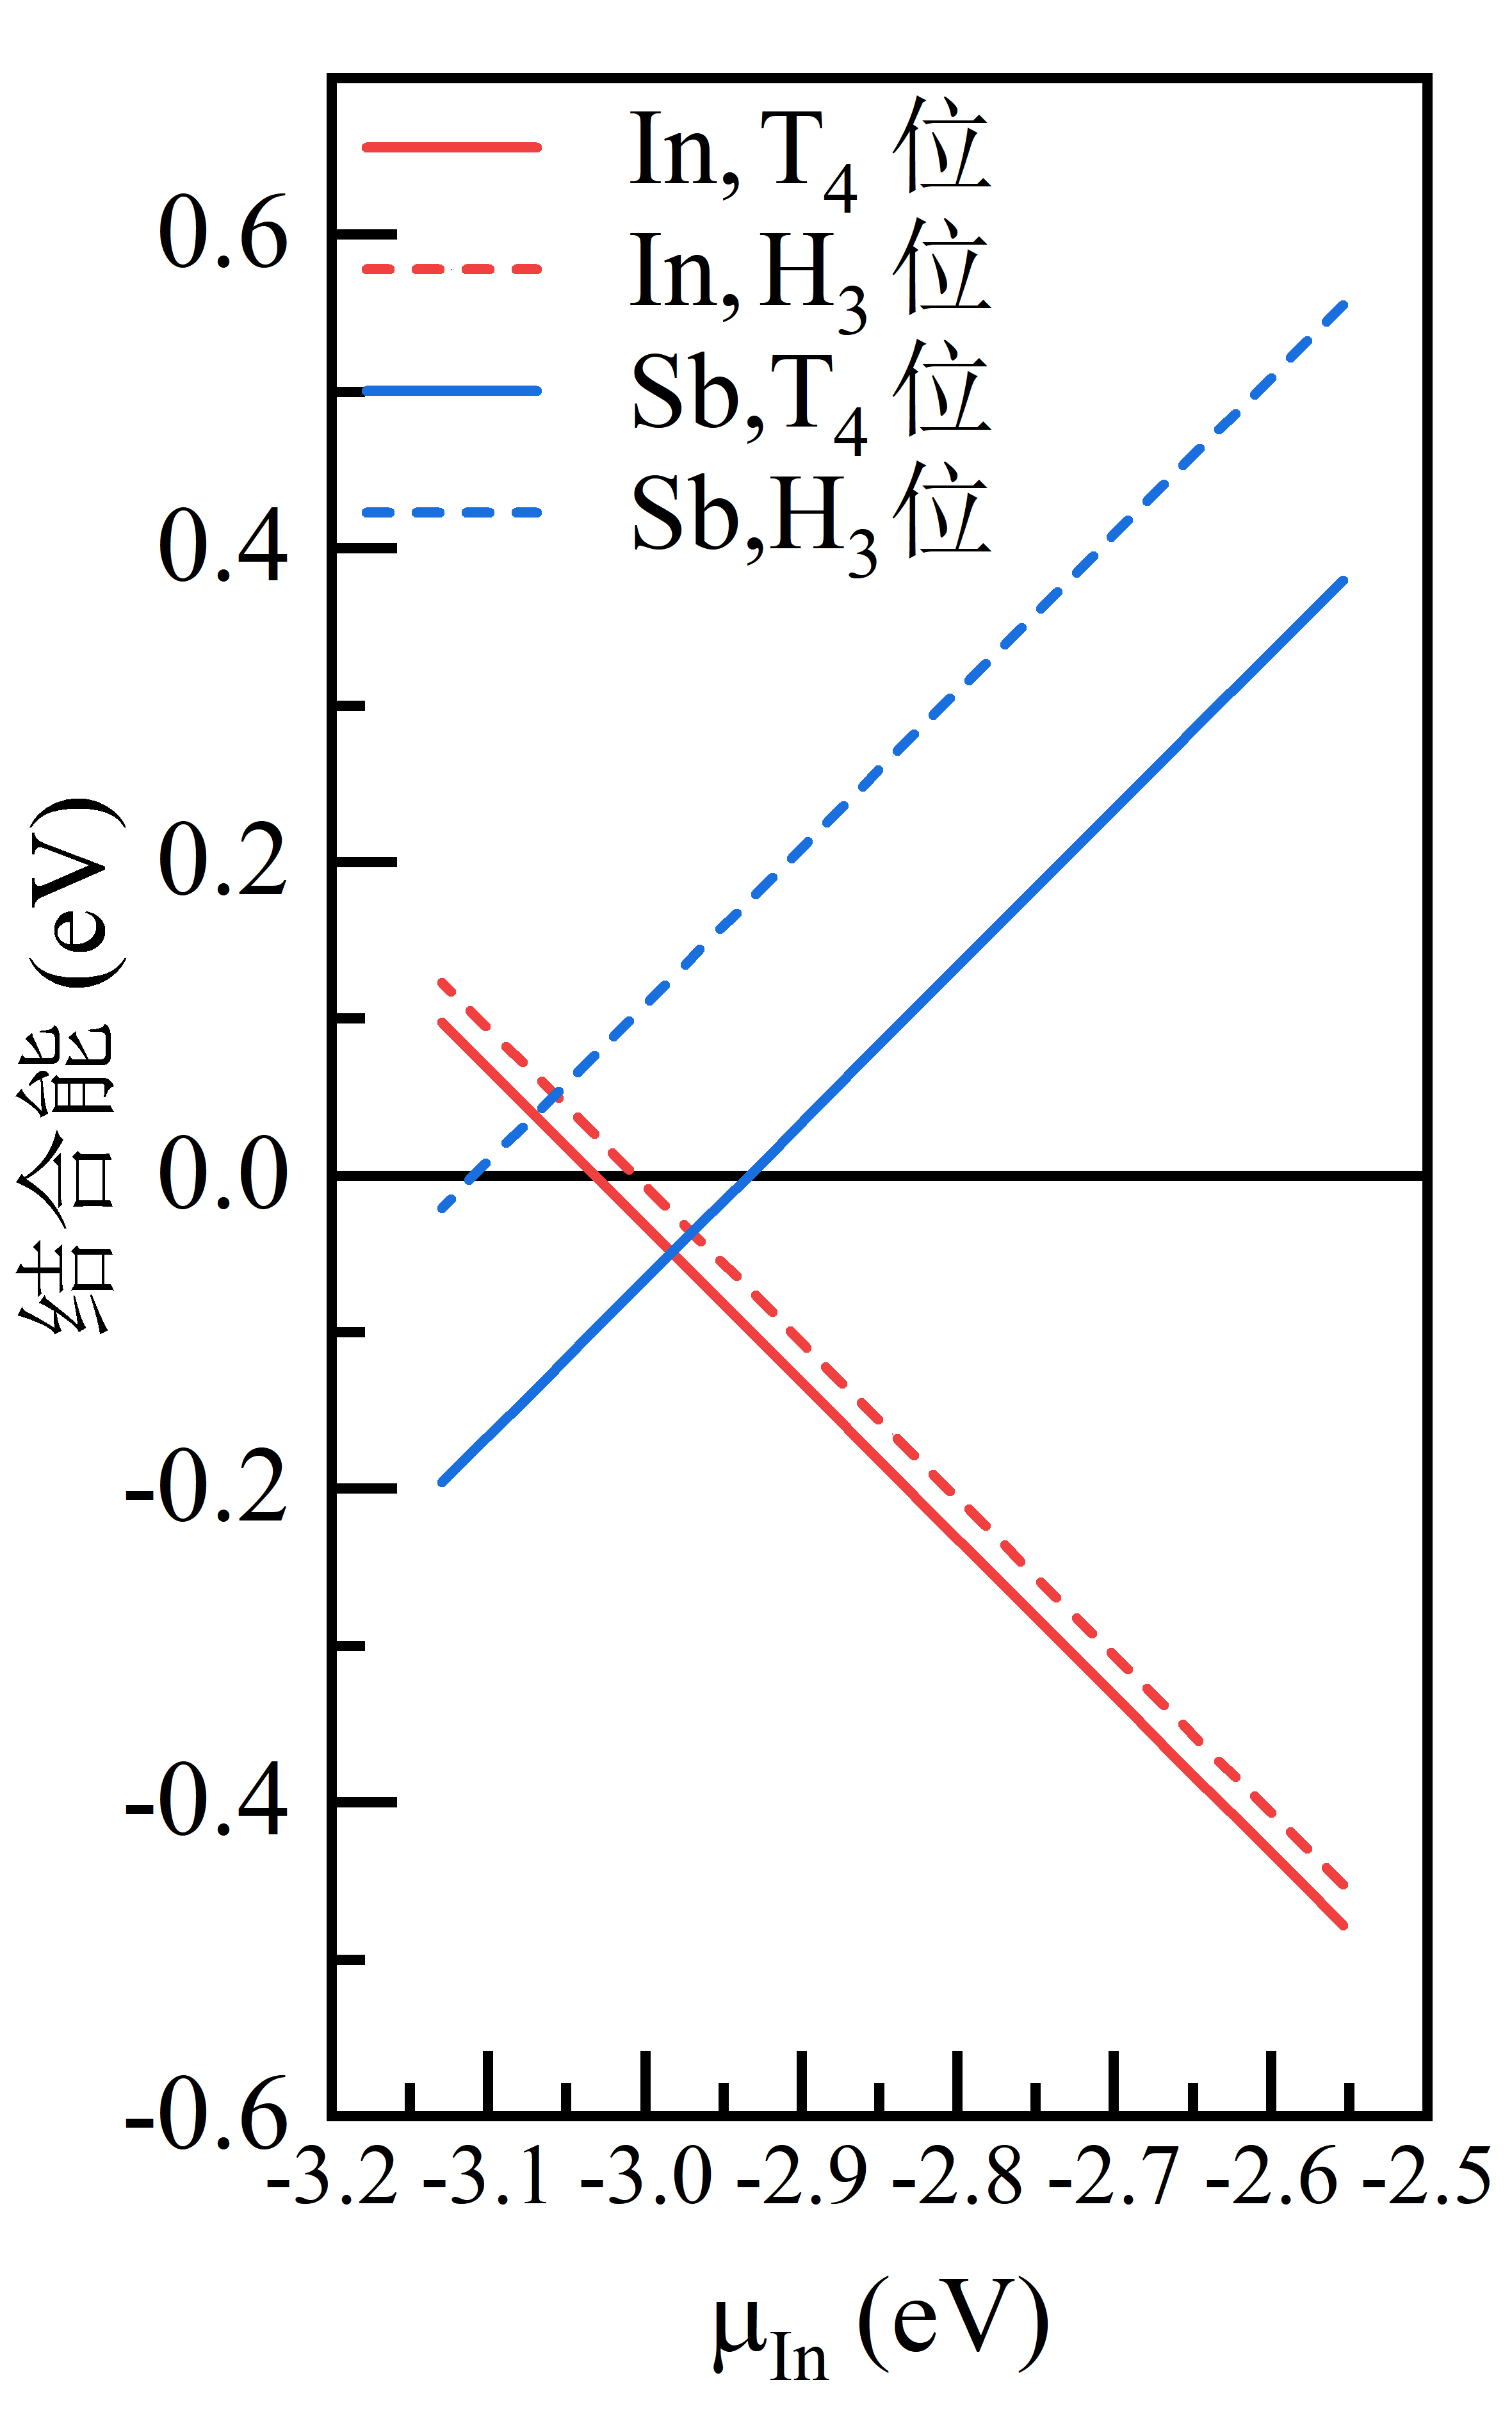
\includegraphics[]{pic/IS_DFT_adatomBind.png}
    }
    \subfloat[]{
        \label{fig:IS_structure_T4onBi}
        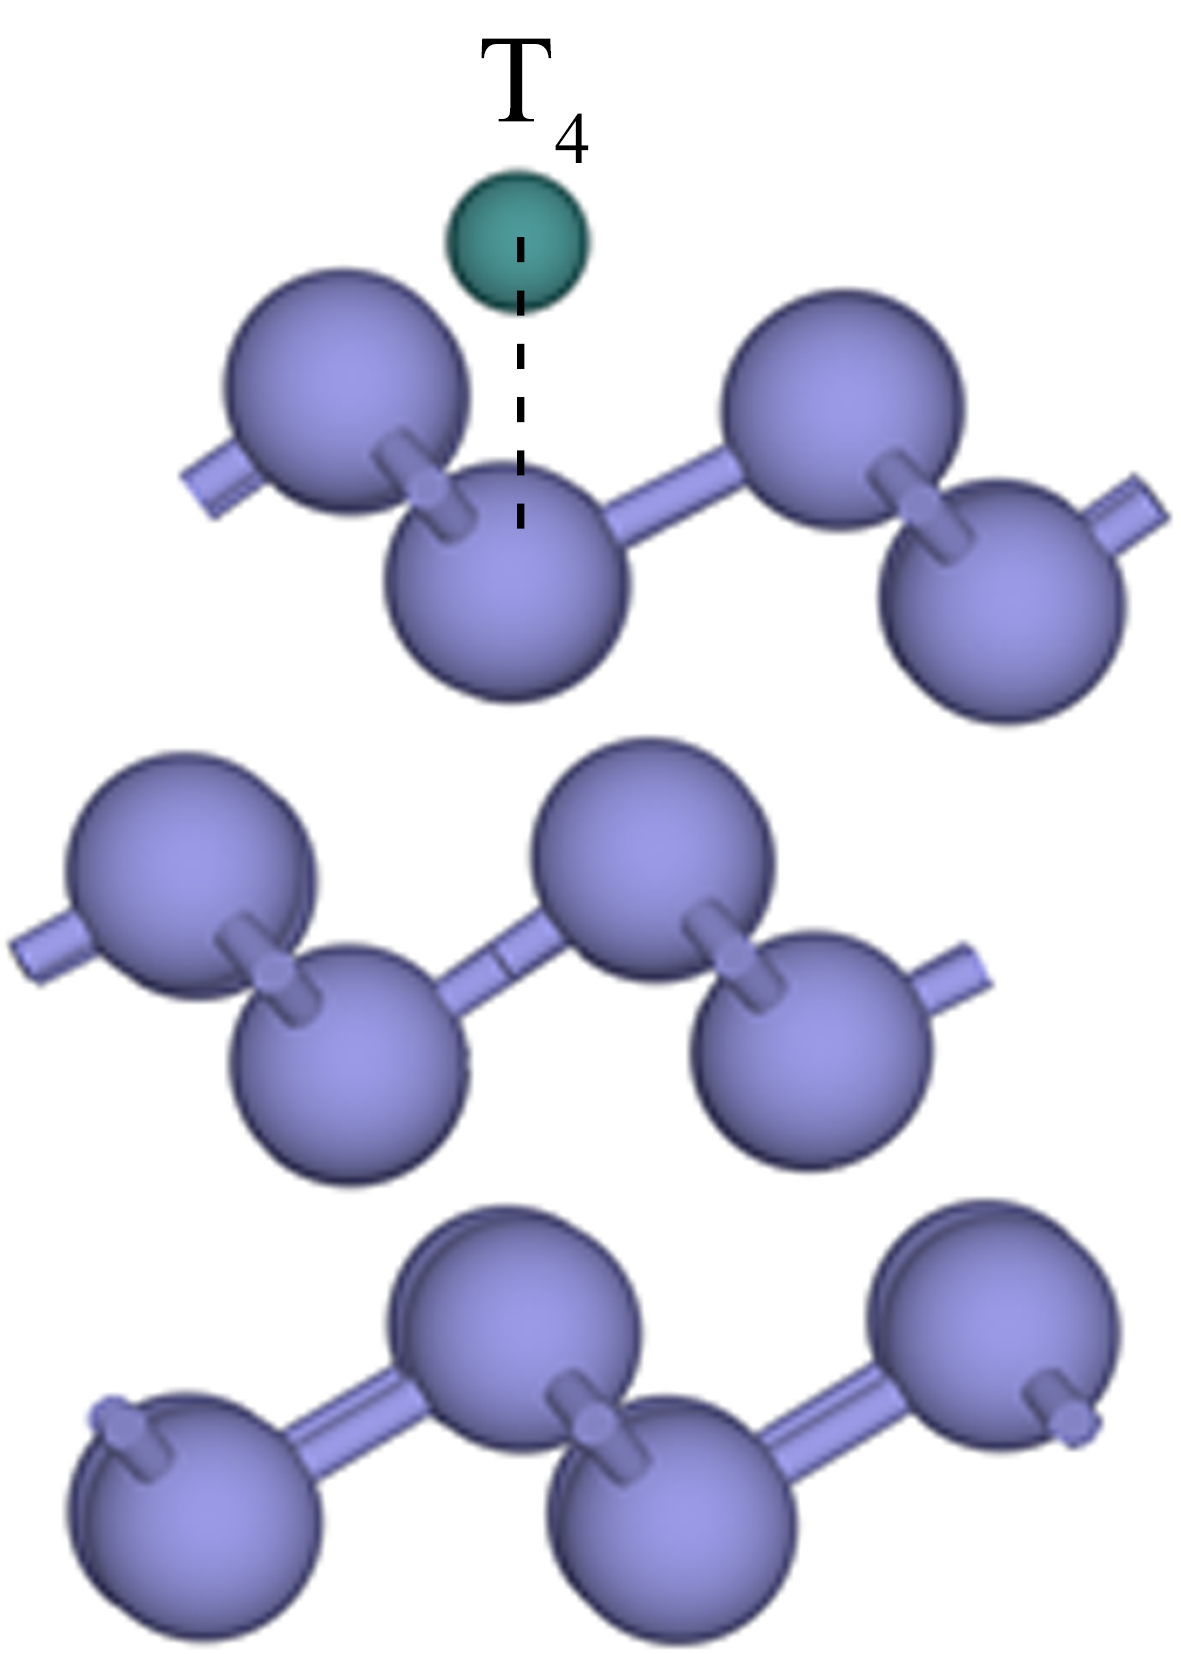
\includegraphics[width=0.3\textwidth,trim={0, -20, 0 0},clip]{pic/IS_structure_T4onBi.png}
    }
    \subfloat[]{
        \label{fig:IS_structure_H3onBi}
        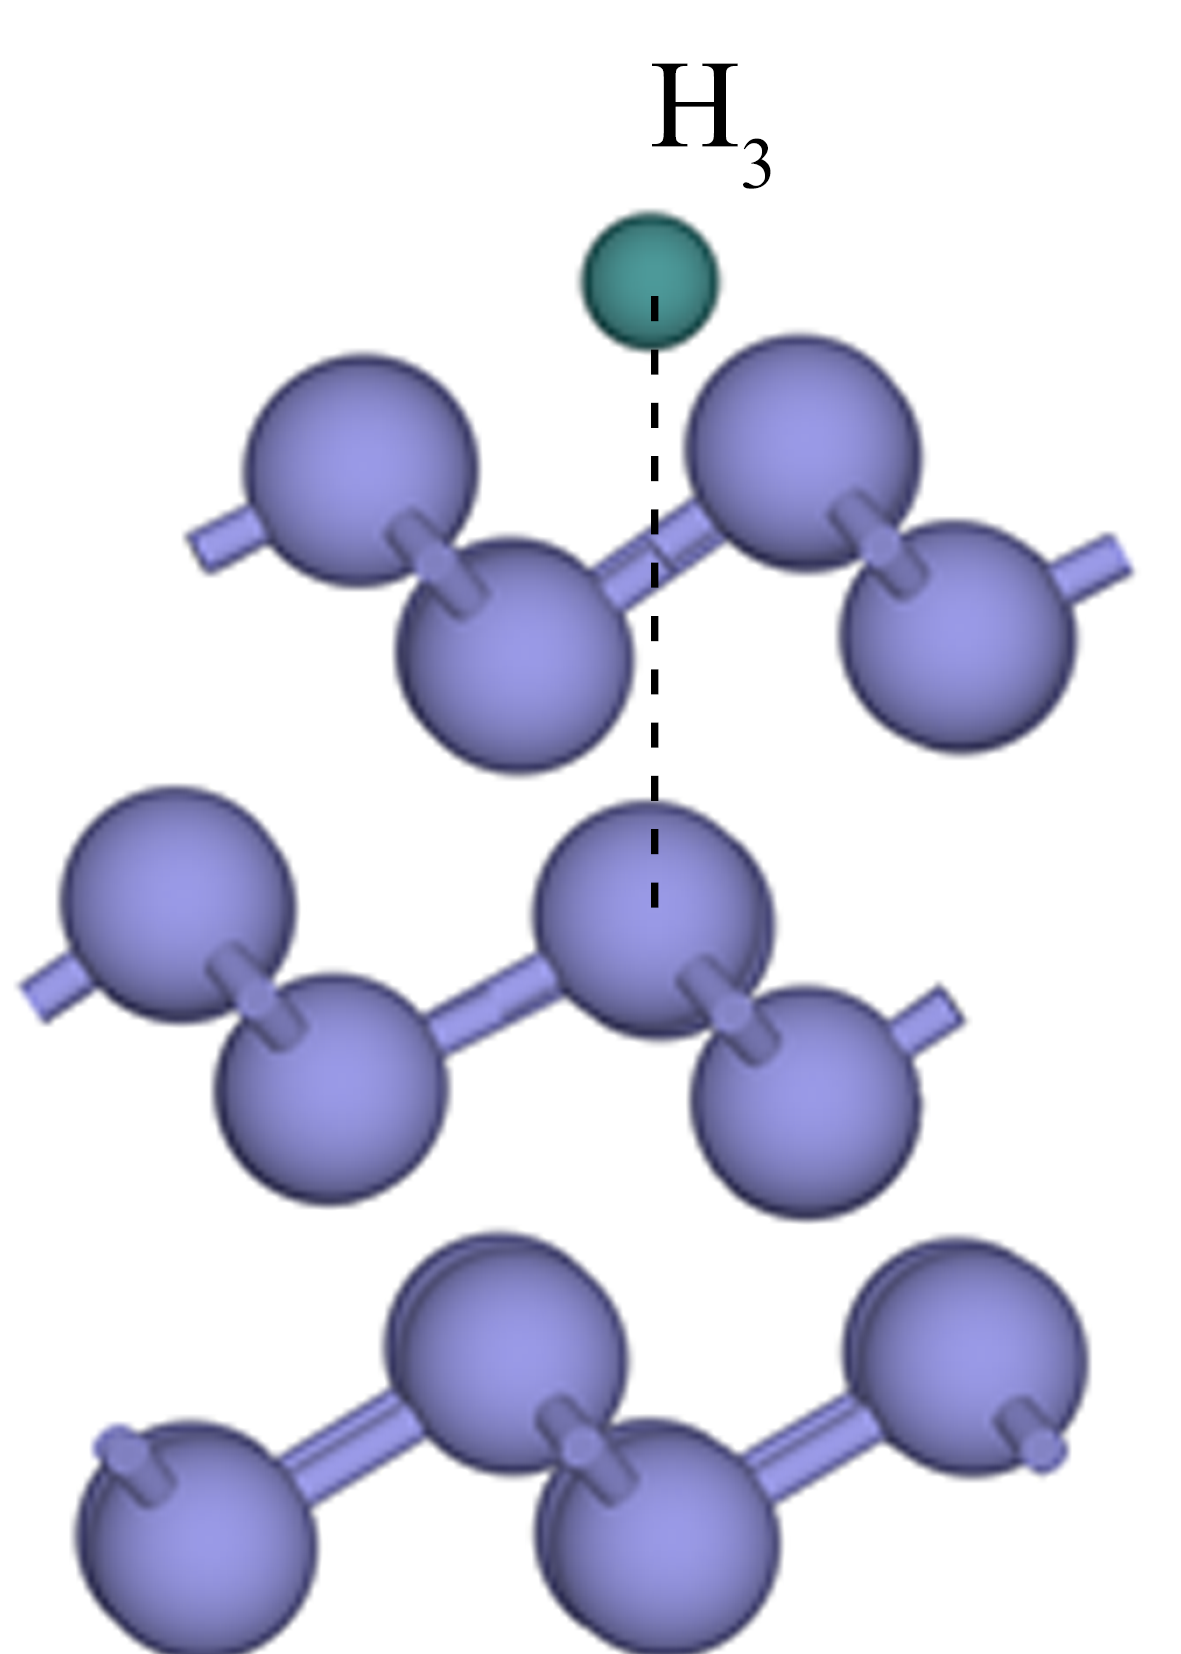
\includegraphics[width=0.3\textwidth,trim={0, -20, 0 0},clip]{pic/IS_structure_H3onBi.png}
    }
    \caption{\cemb{Bi(001)}衬底表面\cemb{In}和\cemb{Sb}吸附原子的结合能和吸附位点。(a)吸附原子结合能;(b)吸附位点T4;(c)吸附位点H3。 原子结构图中,\cemb{Bi}原子使用蓝色表示,吸附原子(\cemb{In}、\cemb{Sb})用绿色表示}
    \label{fig:IS_Bi_adatoms}
\end{figure}

考虑\cemb{In}和\cemb{Sb}吸附原子在\cemb{Bi(001)}表面吸附覆盖率为$1/ 4$的结合能,计算结果如\ref{fig:IS_Bi_adatoms}所示。根据本文的计算,\cemb{In}原子和\cemb{Sb}原子都更倾向于吸附在\cemb{Bi(001)}衬底表面的$\TfourSite$位和$\HthreeSite$位。如图\ref{fig:IS_structure_T4onBi}和\ref{fig:IS_structure_H3onBi}所示,$\TfourSite$为\cemb{Bi(001)}衬底表面的四重配位顶位,正对于第一层\cemb{Bi}双原子层的下层原子。$HthreeSite$为\cemb{Bi(001)}衬底表面的三种配位空心位,正对于第一层\cemb{Bi}双原子层的空心以及第二层\cemb{Bi}双原子层的上层原子。\cemb{In}原子和\cemb{Sb}原子在\cemb{Bi(001)}衬底表面的吸附能如图\ref{fig:IS_DFT_adatomBind}所示,计算表明\cemb{Bi(001)}衬底表面的$\TfourSite$为\cemb{In}原子和\cemb{Sb}原子的最佳吸附位点。而$\HthreeSite$为二者的次优吸附位点。在吸附能以及后续的能量计算中,本文使用\cemb{In}的化学势$\muVar{In}{}$来表示\cemb{In}元素在生长气氛中的活性水平,体现在\cemb{InSb}化学平衡下\cemb{In}元素和\cemb{Sb}元素的浓度差距。

对于$\muVar{adatom}{}$为吸附原子的化学势,由于生长环境下\cemb{InSb}块体的化学平衡,有\chinesecolon
\begin{equation}
    \label{eq:IS_bulkEqmb}
    \muVar{In}{}+\muVar{Sb}{}=\energyVar{InSb}{tot}=\energyVar{In\left(Bulk\right)}{}+\energyVar{Sb\left(Bulk\right)}{}+\rm{\Delta} \it H_{\rm f}\left(\ce{InSb}\right)
\end{equation}
其中$\energyVar{InSb}{tot}$、$\energyVar{In\left(Bulk\right)}{}$和$\energyVar{Sb\left(Bulk\right)}{}$为\cemb{InSb}块体,\cemb{In}块体和\cemb{Sb}块体的能量。因此,在生长气氛中\cemb{InSb}的化学平衡下,$\muVar{In}{}$的变化范围为$ \energyVar{In\left(Bulk\right)}{}+\rm{\Delta} \it H_{\rm f}\left(\ce{InSb}\right) \leqslant \muVar{In}{} \leqslant \energyVar{In\left(Bulk\right)}{}$,代表\cemb{In}的化学势$\muVar{In}{}$由纯\cemb{Sb}的生长环境变化到纯\cemb{In}的生长环境。

对于吸附在$\TfourSite$位点的\cemb{In}原子,计算所得的在纯\cemb{In}环境下的结合能为\SI{-0.48}{\electronvolt},低于在纯\cemb{Sb}环境下同样吸附在$\TfourSite$位点的\cemb{Sb}原子的结合能(\SI{-0.19}{\electronvolt})。更抵的结合能意味着相比于\cemb{Sb}原子,在能量最低的驱动下有更多的\cemb{In}原子从块体的状态分离并以吸附原子的状态沉积到\cemb{Bi(001)}的表面。对于\cemb{In}原子来说,其在最优吸附位点$\TfourSite$的结合能只比吸附次优吸附位点$\HthreeSite$的结合能低\SI{0.026}{\electronvolt}。而对于\cemb{Sb}原子,其在次优吸附点$\HthreeSite$和最优吸附点$\TfourSite$之间的结合能之差为\SI{0.17}{\electronvolt}。由于\cemb{Sb}原子在次优吸附位点$\HthreeSite$较差的吸附能力,\cemb{Sb}原子只能在接近纯\cemb{Sb}的生长环境中在\cemb{Bi(001)}表面的$\HthreeSite$位点吸附。

进一步考虑生长环境中的化学计量比的变化对于原子吸附的影响。在图\ref{fig:IS_DFT_adatomBind}中可以看到,只有很小的$\muVar{In}{}$区间允许\cemb{In}和\cemb{Sb}同时在\cemb{Bi(001)}衬底表面吸附($\energyVar{f}{} \leqslant 0$)。在这个区间内\cemb{In}原子可以在$\TfourSite$和$\HthreeSite$位点吸附,而\cemb{Sb}原子只能在$\HthreeSite$位点吸附。对于\cemb{In}原子,由于较低的吸附能,相比于\cemb{Sb}原子其能够在较宽的$\muVar{In}{}$区间内在\cemb{Sb}衬底表面吸附。当环境中的\cemb{In}原子化学势稍微向纯\cemb{In}环境倾斜时($\muVar{In}{}\geqslant \SI{-2.9}{\electronvolt}$),仅有\cemb{In}能够在\cemb{Bi}的表面吸附,而\cemb{Sb}原子则由于大于零的结合能倾向于从\cemb{Bi}的表面脱附。

由于\cemb{In}原子和\cemb{Sb}原子在\cemb{Bi(001)}表面不同的吸附行为,在相同的化学气氛下,\cemb{In}和\cemb{Sb}很难同时在\cemb{Bi}衬底的表面独立吸附。出于更高的吸附能力,\cemb{In}在\cemb{InSb}的初期成核生长过程中处于更加主导的地位。在\cemb{In}原子能够沉积的区域,气氛中的\cemb{Sb}原子需要与已吸附的\cemb{In}原子成键、成核,才能够在\cemb{Bi}衬底的表面形成\cemb{InSb}。

\begin{figure}[htb]
    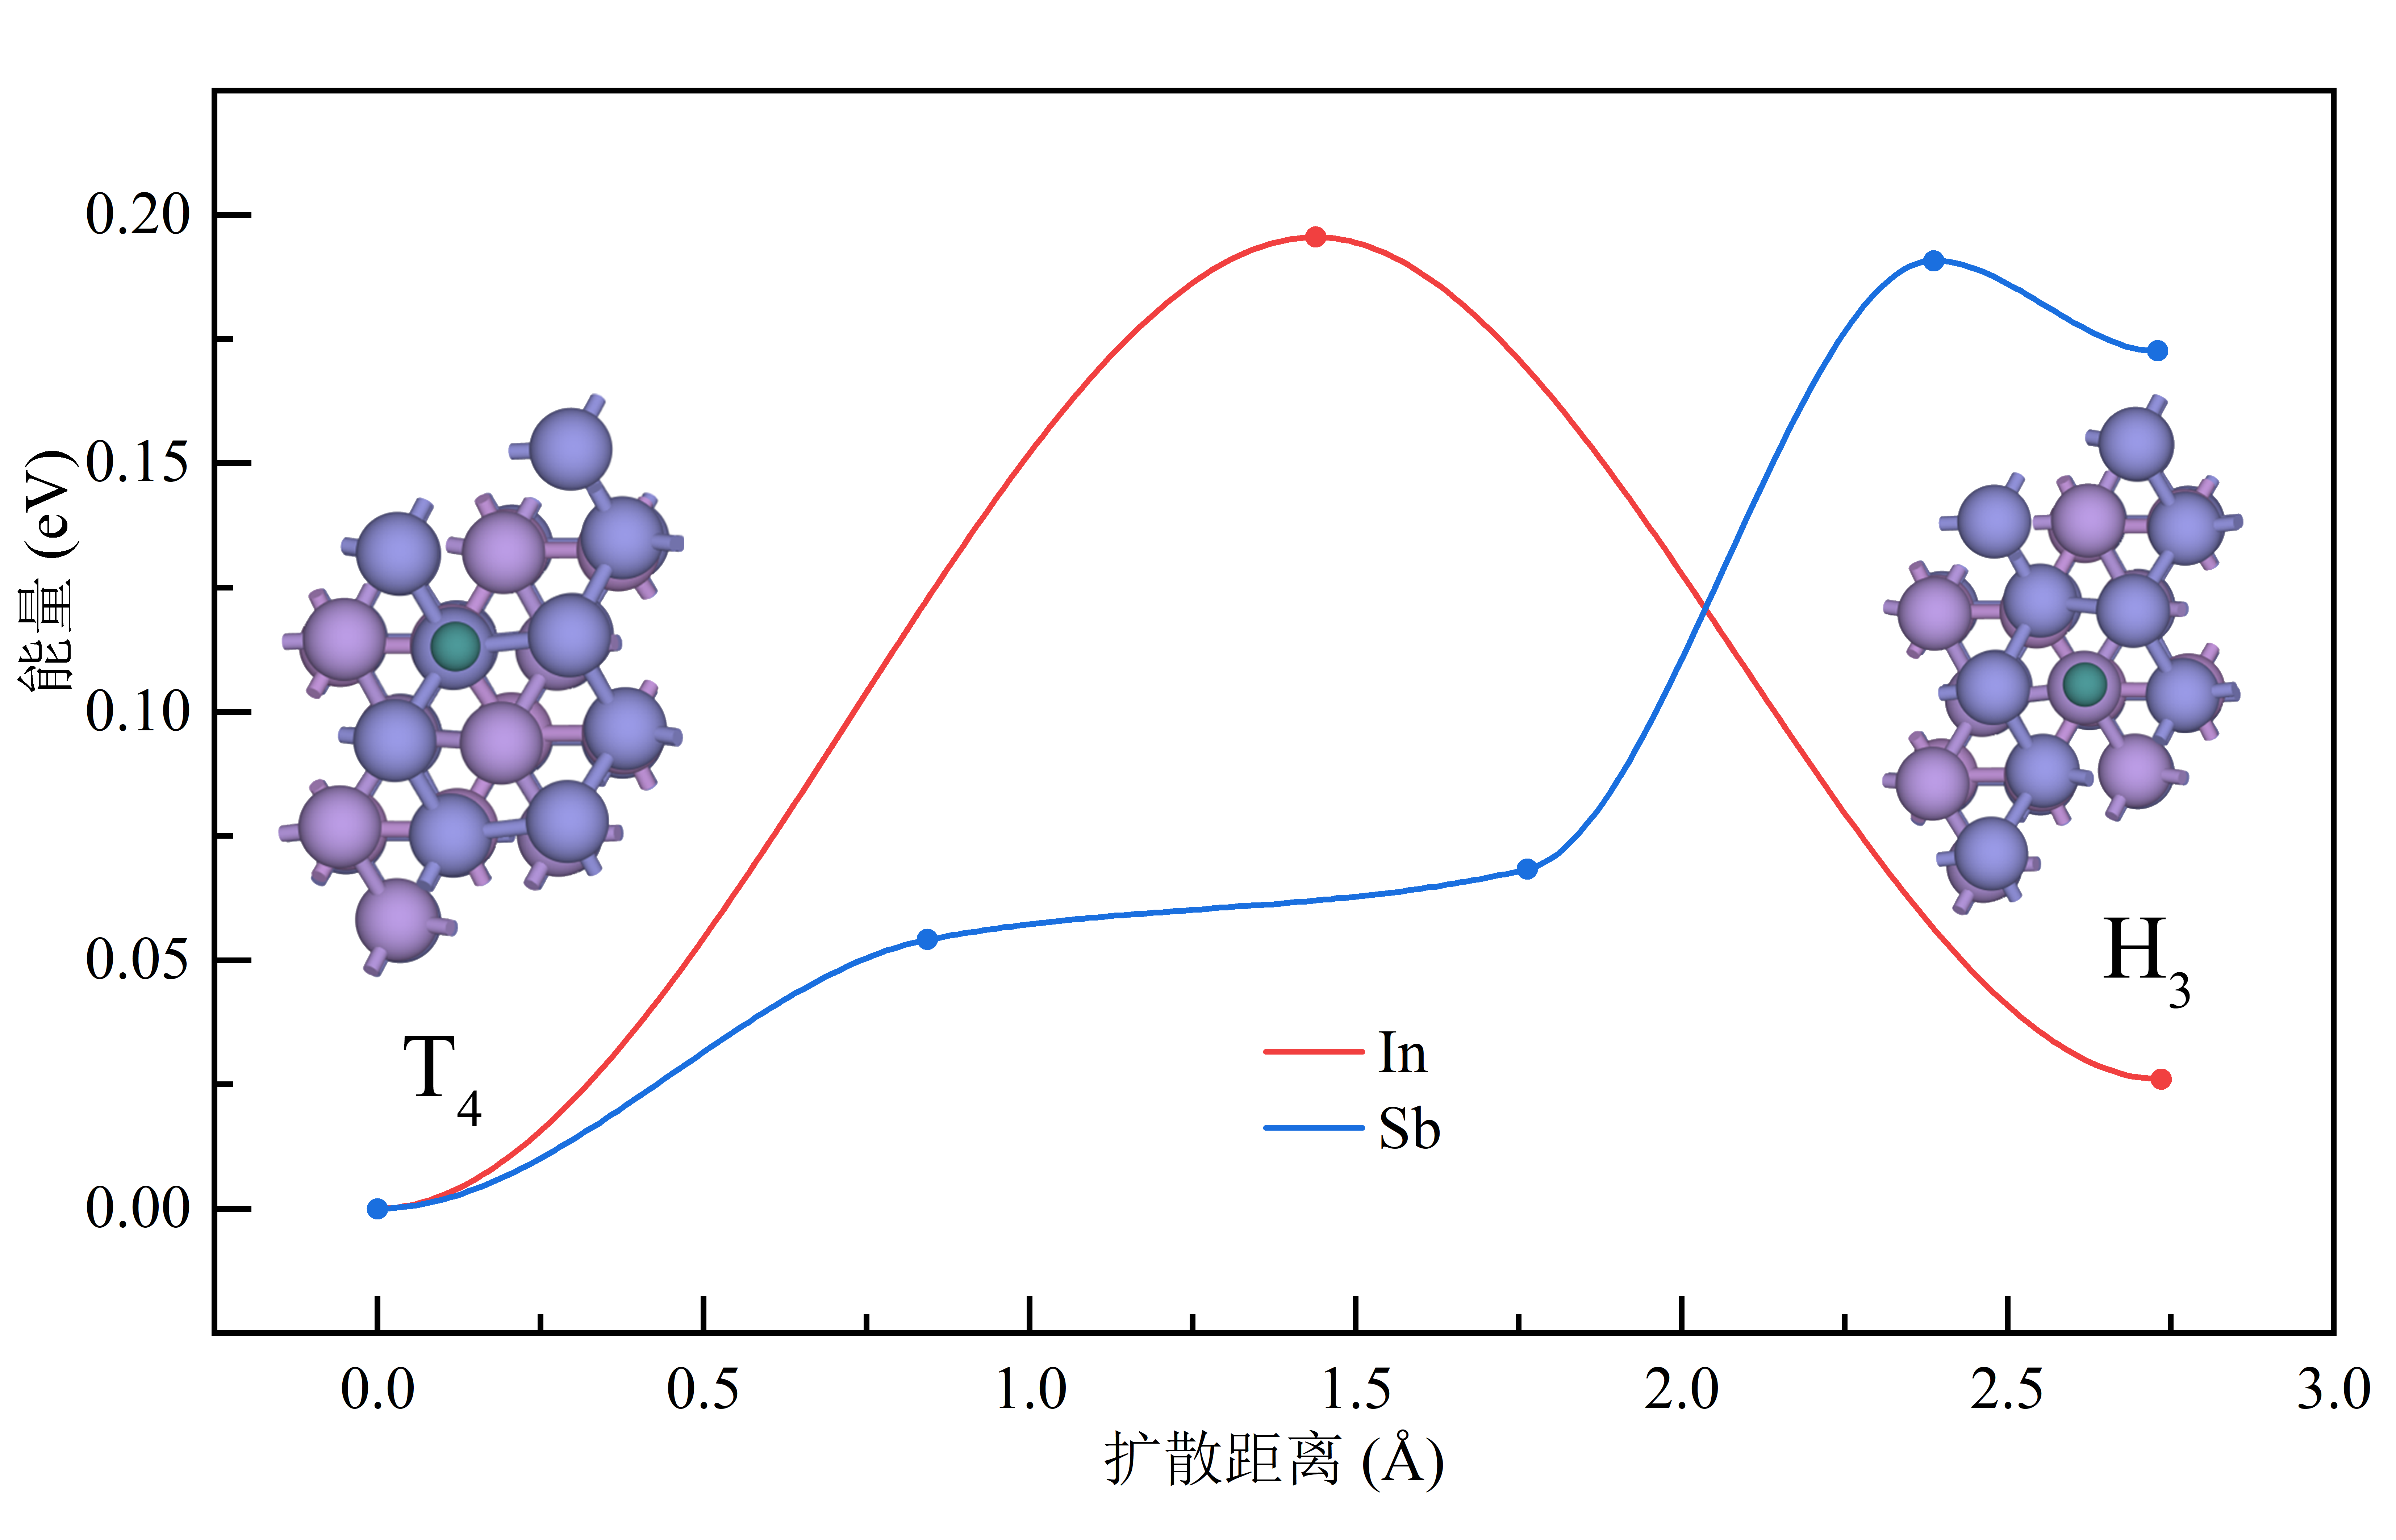
\includegraphics{pic/IS_DFT_adatomDiff.png}
    \caption{\cemb{Bi(001)}衬底表面\cemb{In}和\cemb{Sb}吸附原子的迁移势垒。原子结构图中,\cemb{Bi}原子使用蓝色表示,吸附原子(\cemb{In}、\cemb{Sb})用绿色表示}
    \label{fig:IS_DFT_adatomDiff}
\end{figure}


本文进一步计算了\cemb{In}和\cemb{Sb}原子吸附在\cemb{Bi(001)}表面后的迁移势垒。如图\ref{fig:IS_DFT_adatomDiff}所示,对于吸附在\cemb{Bi}衬底表面的\cemb{In},其在两个等效的最优吸附$\TfourSite$位点之间迁移的势垒为\SI{0.20}{\electronvolt}。对于\cemb{Sb}原子,其在同样的最优位点$\TfourSite$之间的迁移势垒略低,为$\SI{0.19}{\electronvolt}$。而对于吸附在次优吸附位点$\HthreeSite$的\cemb{Sb}原子,只需要跨越\SI{0.018}{\electronvolt}的势垒就可迁移至最优的$\TfourSite$位点。吸附在$\HthreeSite$位点的\cemb{In}原子需要跨越约\SI{0.17}{\electronvolt}的势垒即可可迁移至能量更有优势的$\HthreeSite$位点。考虑到\cemb{In}原子在最优吸附位点$\TfourSite$和次优吸附位点$\HthreeSite$之间的能量差只有\SI{0.026}{\electronvolt},并且\cemb{In}原子和\cemb{Sb}原子在\cemb{Bi(001)}表面较低的迁移势垒,吸附的\cemb{In}原子在$\TfourSite$和$\HthreeSite$近似于均匀分布。而\cemb{Sb}原子由于在$\TfourSite$位点具有约\SI{0.17}{\electronvolt}的能量优势,因此\cemb{Sb}原子在$\TfourSite$位点吸附的比例较高。

为了能进一步探究\cemb{InSb(111)}在\cemb{Bi(001)}衬底上的层状生长机理以及极性的演化过程,本文计算了单层\cemb{InSb}在\cemb{Bi(001)}衬底上的形成能$\energyVar{f}{}$\chinesecolon
\begin{equation}
    \label{eq:IS_formationEnenrgy}
    \energyVar{f}{}=\frac{1}{\alpha}\left(\energyVar{\cemb{InSb}+sub}{}-\energyVar{sub}{}-N_{\rm In}\muVar{In}{}-N_{\rm Sb}\muVar{Sb}{}\right)
\end{equation}
其中,$\alpha$为模拟体系的表面积;$\energyVar{\cemb{InSb}+sub}{}$和$\energyVar{sub}{}$分别为在衬底表面生长了一层\cemb{InSb}的能量以及单独衬底的能量;$N_{\rm In}$和$N_{\rm Sb}$分别为\cemb{InSb}单层中\cemb{In}和\cemb{Sb}原子的数量。

本文首先考虑理想的\cemb{InSb}单层在\cemb{Bi(001)}衬底上的生长情况。在计算中,无论是\cemb{In}极性的\cemb{InSb(111)}单层还是\cemb{Sb}极性,他们都倾向于在\cemb{Bi(001)}衬底表面形成面心立方的堆叠形式(fcc, ABC堆叠)。同时,这也与本文在单\cemb{In/Sb}原子的吸附计算结果一致,即\cemb{In}和\cemb{Sb}作为吸附原子更倾向于吸附在\cemb{Bi(001)}表面的$\TfourSite$位和$\HthreeSite$位。具体而言,\cemb{In}极性的\cemb{InSb(111)}单层在\cemb{Bi(001)}衬底的表面形成能为\SI{-13.74}{\mievpas},高于\cemb{Sb}极性\cemb{InSb(111)}单层的\SI{-9.40}{\mievpas}。因此,对于理想的\cemb{InSb}单层,在\cemb{Bi(001)}衬底上应生长为\cemb{In}极性。在表格\ref{tab:IS_idealInSb_formationEnergy}中,本文总结了不同极性的\cemb{InSb}单层在\cemb{Bi(001)}衬底上的形成能及原子分布。

\begin{table}[htb]
    \centering
    \caption{不同极性的\cemb{InSb}单层在\cemb{Bi(001)}衬底上的形成能及原子分布}
    \begin{tabular}{
        m{0.15\textwidth}
        m{0.25\textwidth}
        m{0.22\textwidth}
        m{0.22\textwidth}
    }
        \toprule
        极性          & 形成能(\si{\mievpas}) & \cemb{In}原子位置 & \cemb{Sb}原子位置 \\
        \midrule
        \cemb{In}极性 & -13.74                & $\TfourSite$      & $\HthreeSite$     \\
        \cemb{Sb}极性 & -9.40                 & $\HthreeSite$     & $\TfourSite$      \\
        \bottomrule
    \end{tabular}
    \label{tab:IS_idealInSb_formationEnergy}
\end{table}

\subsection{单层\cemb{InSb}的极性演化}

接着,本文将单层\cemb{InSb(111)}极性的考察范围扩大到非理想的情况。考虑到吸附的\cemb{In}原子和\cemb{Sb}原子均倾向于沉积在$\TfourSite$位点和$\HthreeSite$位点,使用包含四个\cemb{In}原子和四个\cemb{Sb}原子的$2 \times 2$切片模型,可以列举出六种可能的单层\cemb{InSb}极性。在图\ref{fig:IS_structure_1Linsb_allPolarity}中,本文列出了本章中所考虑的所有单层\cemb{InSb}的极性情况。

\begin{figure}[!htb]
    \subfloat[]{
        \label{fig:IS_structure_1Linsb_04}
        \begin{tabular}{c}
            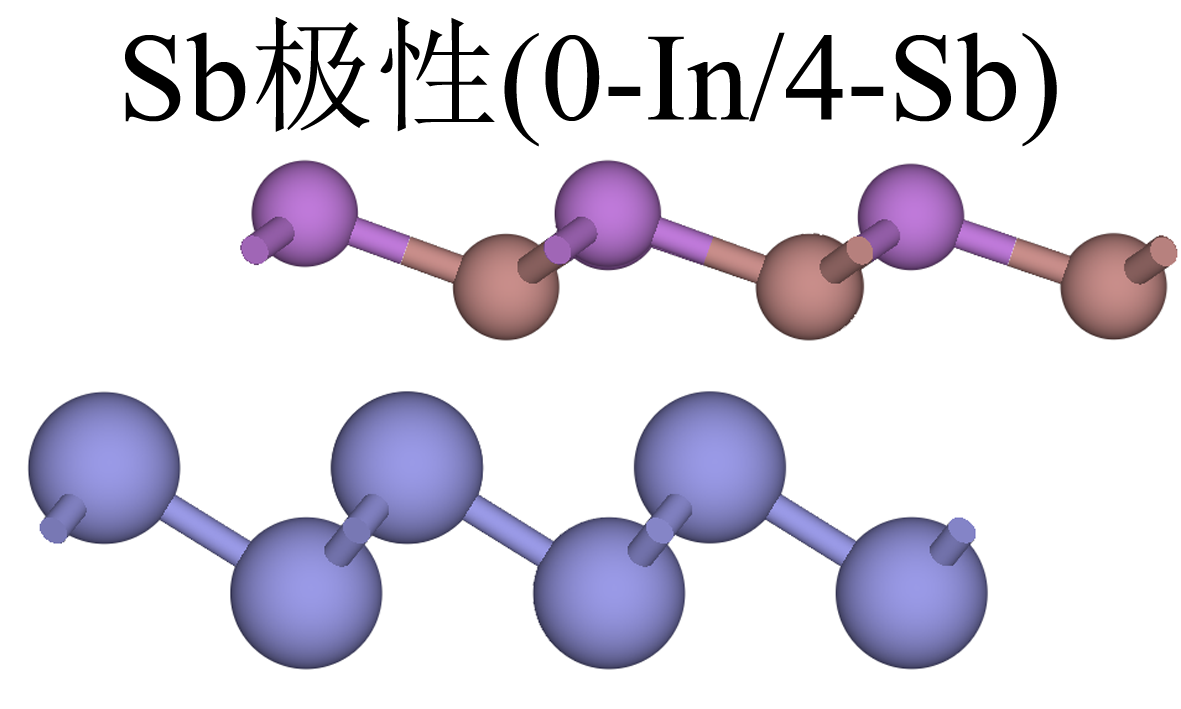
\includegraphics[width=0.27\textwidth]{pic/IS_structure_1Linsb_04side.png} \\[-0.5ex]
            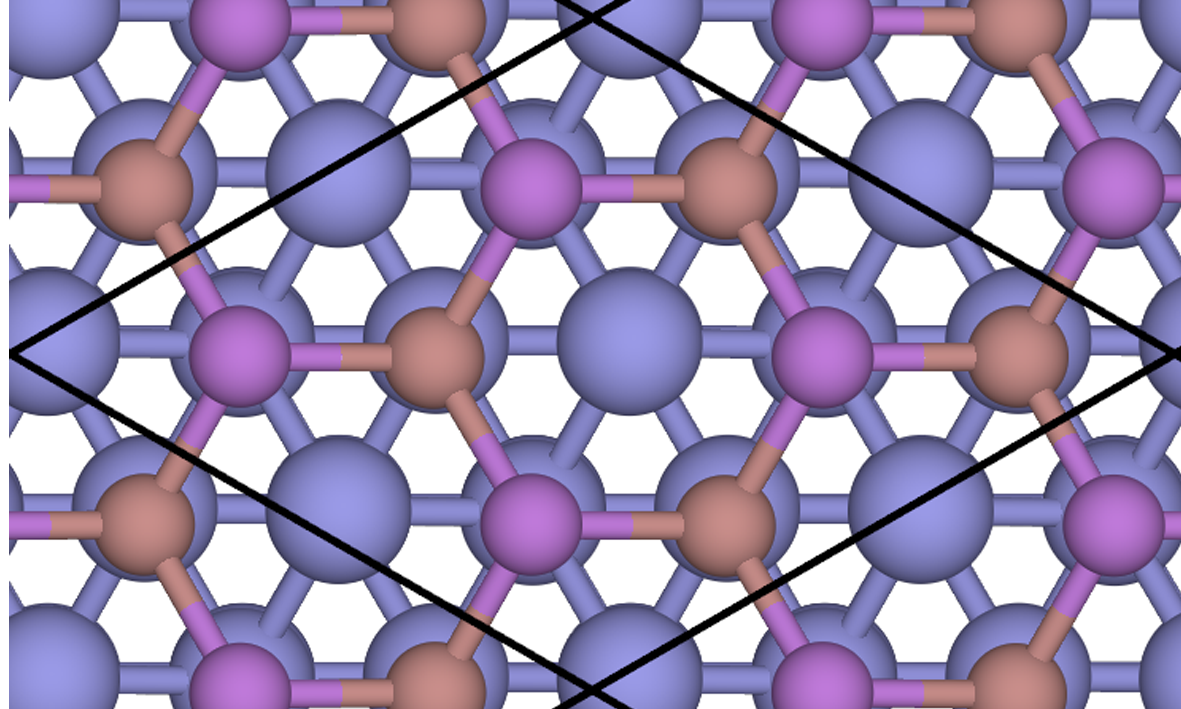
\includegraphics[width=0.27\textwidth]{pic/IS_structure_1Linsb_04top.png}
        \end{tabular}
    }
    \subfloat[]{
        \label{fig:IS_structure_1Linsb_13}
        \begin{tabular}{c}
            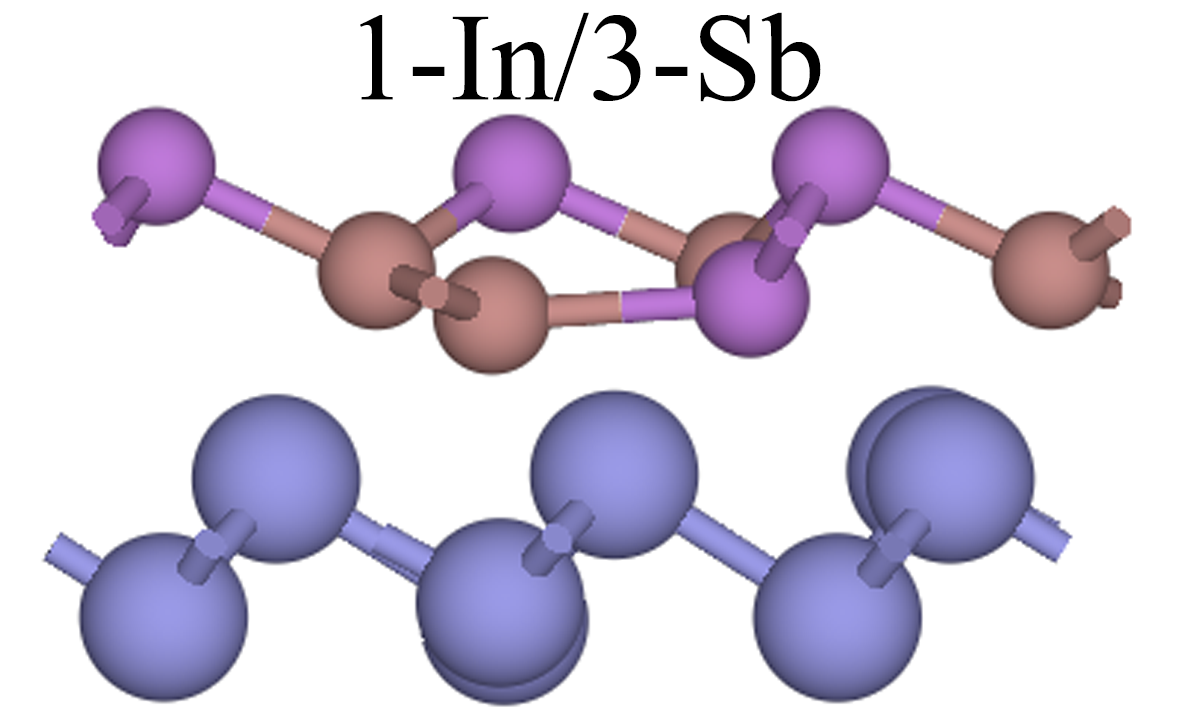
\includegraphics[width=0.27\textwidth]{pic/IS_structure_1Linsb_13side.png} \\[-0.5ex]
            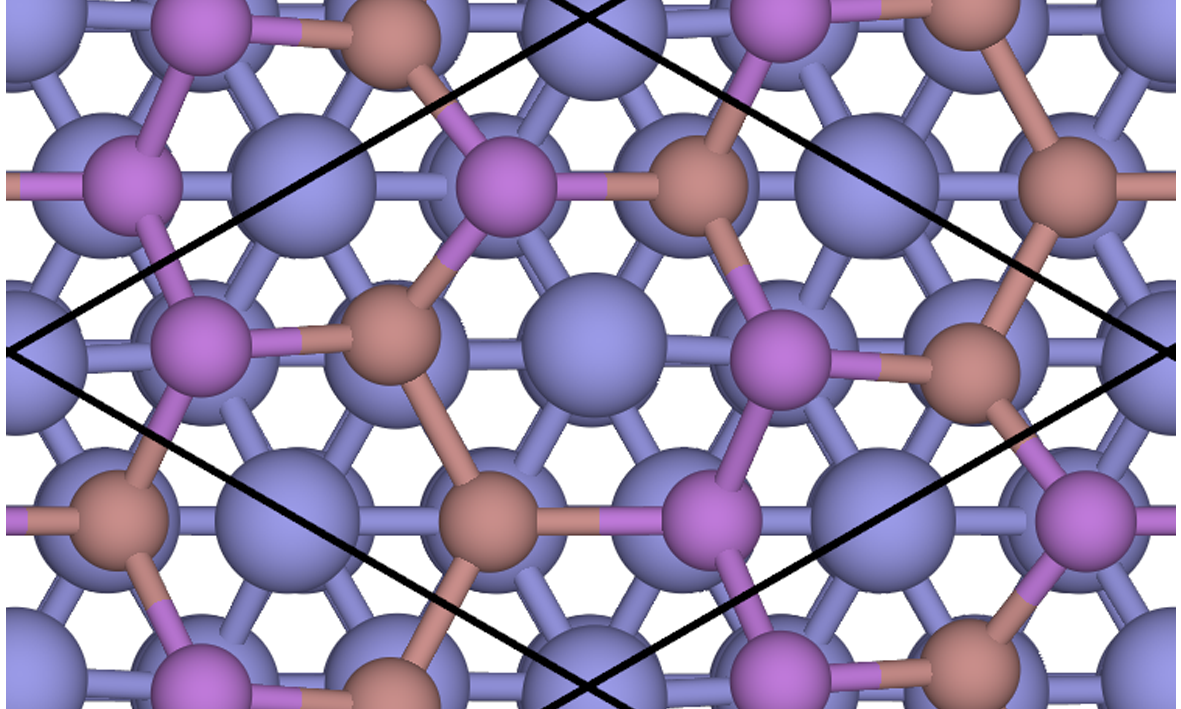
\includegraphics[width=0.27\textwidth]{pic/IS_structure_1Linsb_13top.png}
        \end{tabular}
    }
    \subfloat[]{
        \label{fig:IS_structure_1Linsb_22rec}
        \begin{tabular}{c}
            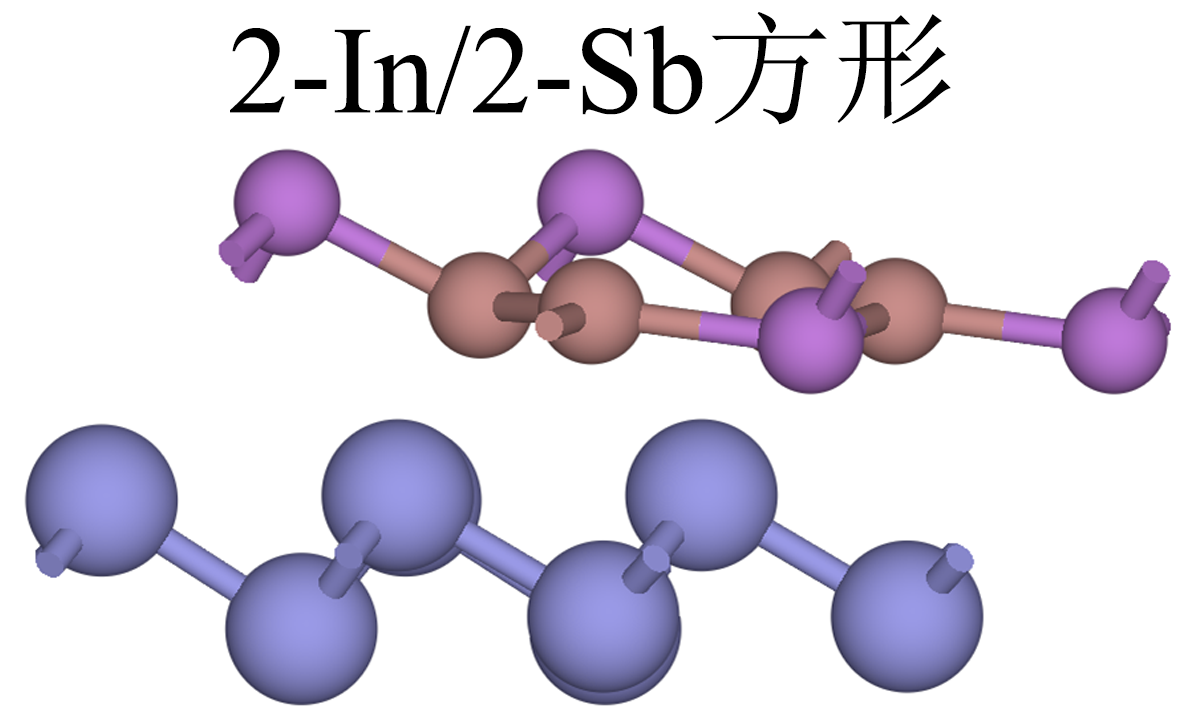
\includegraphics[width=0.27\textwidth]{pic/IS_structure_1Linsb_22recside.png} \\[-0.5ex]
            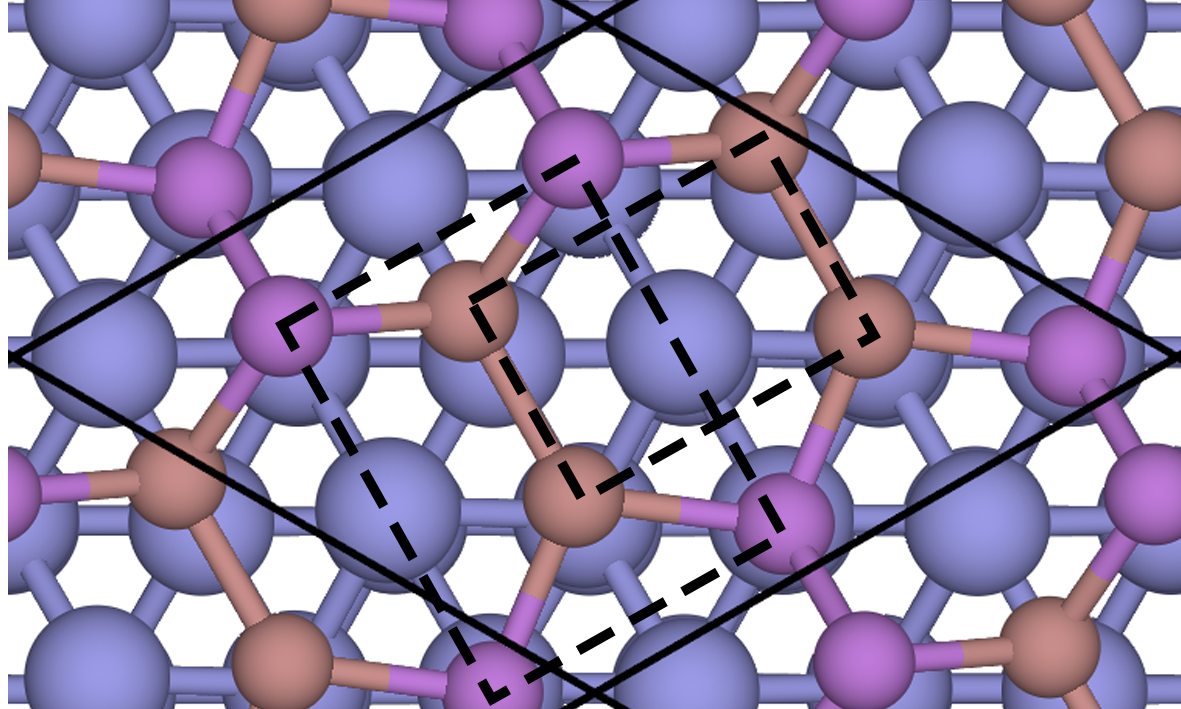
\includegraphics[width=0.27\textwidth]{pic/IS_structure_1Linsb_22rectop.png}
        \end{tabular}
    }\\[-1ex]
    \subfloat[]{
        \label{fig:IS_structure_1Linsb_22str}
        \begin{tabular}{c}
            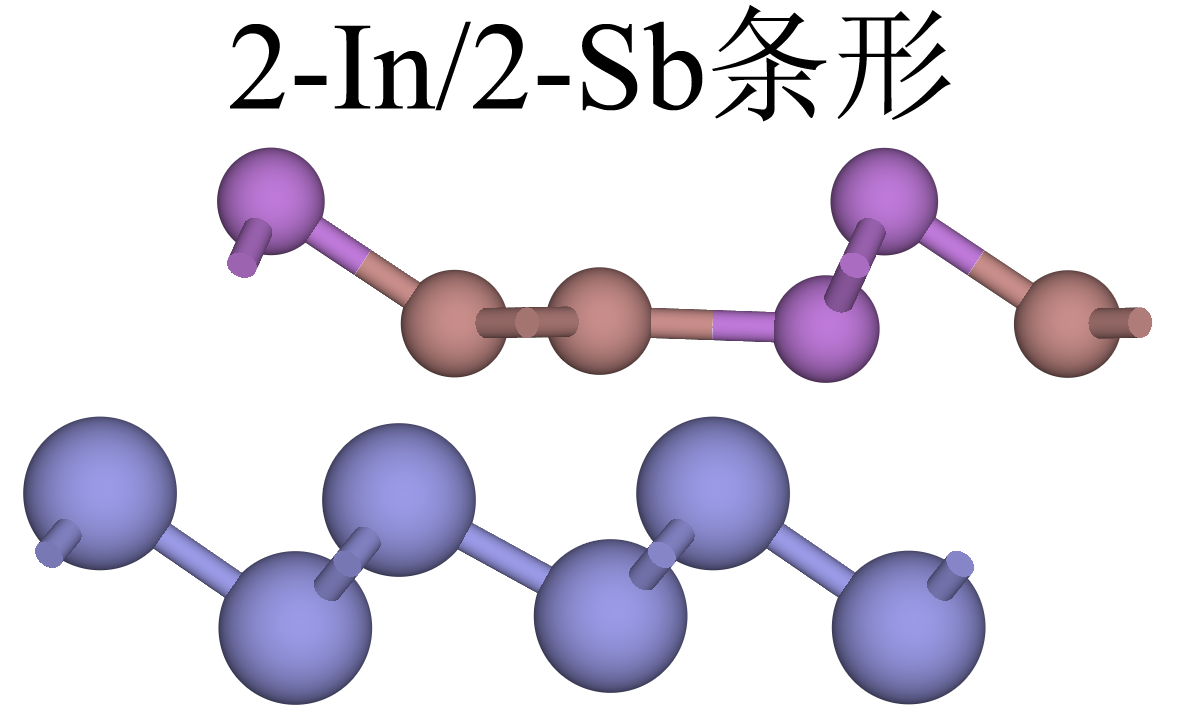
\includegraphics[width=0.27\textwidth]{pic/IS_structure_1Linsb_22strside.png} \\[-0.5ex]
            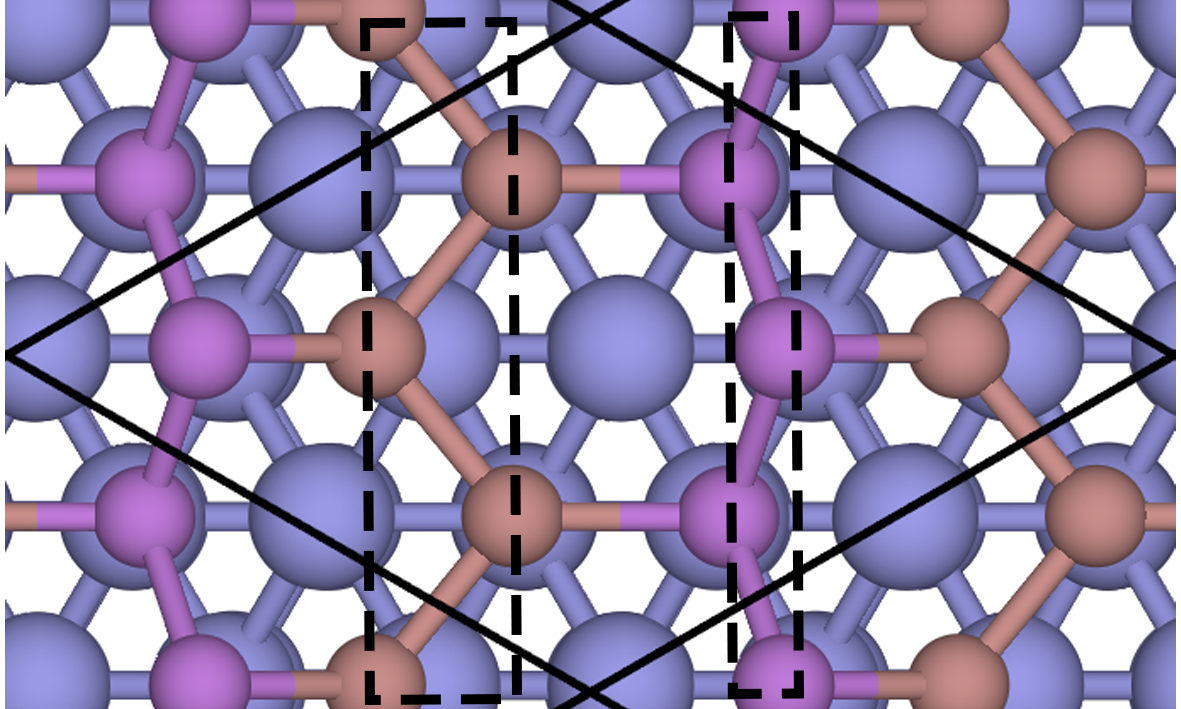
\includegraphics[width=0.27\textwidth]{pic/IS_structure_1Linsb_22strtop.png}
        \end{tabular}
    }
    \subfloat[]{
        \label{fig:IS_structure_1Linsb_31}
        \begin{tabular}{c}
            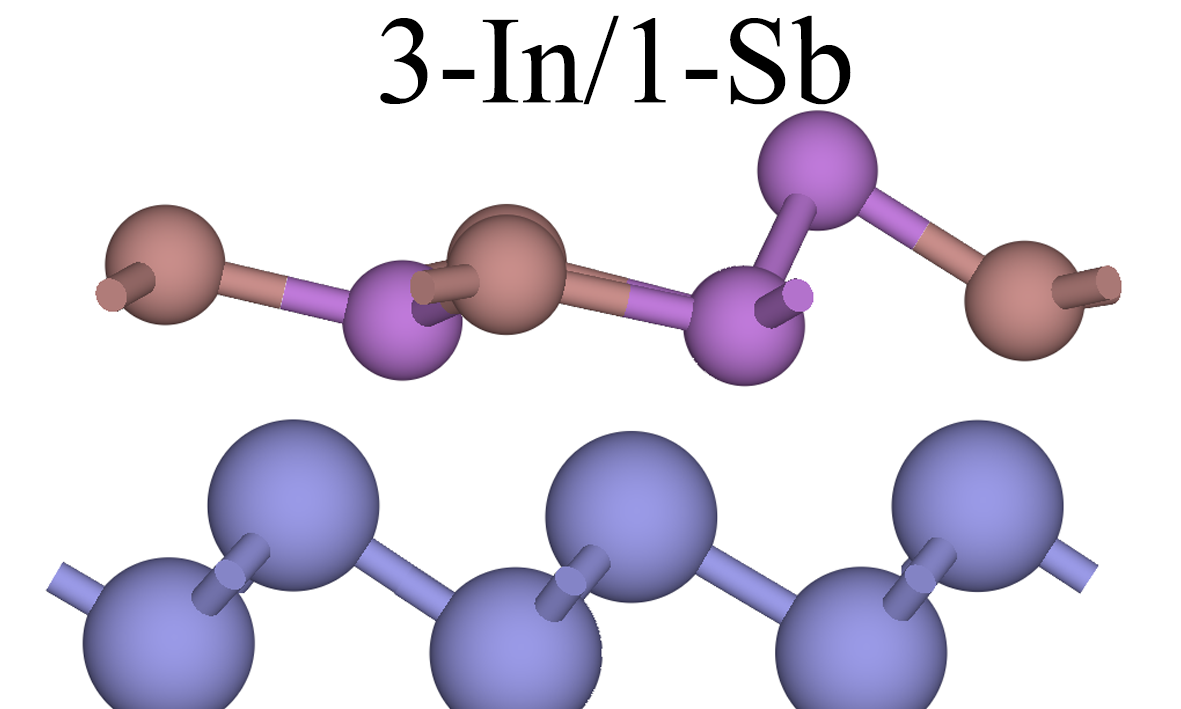
\includegraphics[width=0.27\textwidth]{pic/IS_structure_1Linsb_31side.png} \\[-0.5ex]
            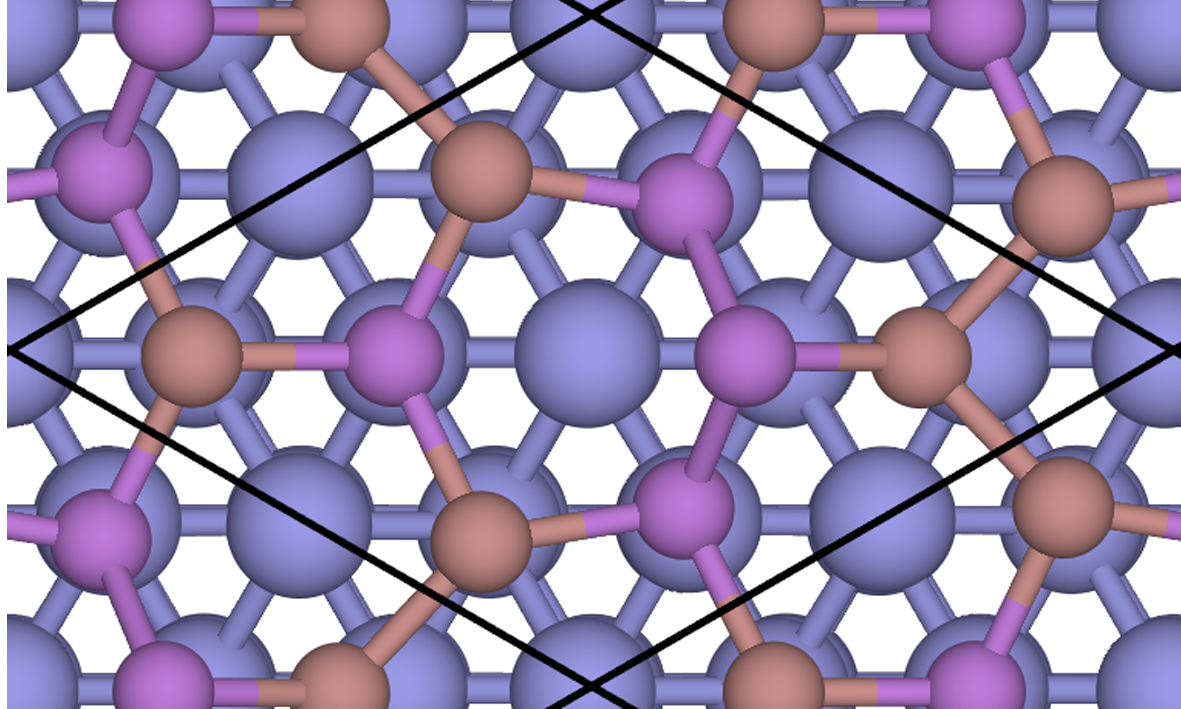
\includegraphics[width=0.27\textwidth]{pic/IS_structure_1Linsb_31top.png}
        \end{tabular}
    }
    \subfloat[]{
        \label{fig:IS_structure_1Linsb_40}
        \begin{tabular}{c}
            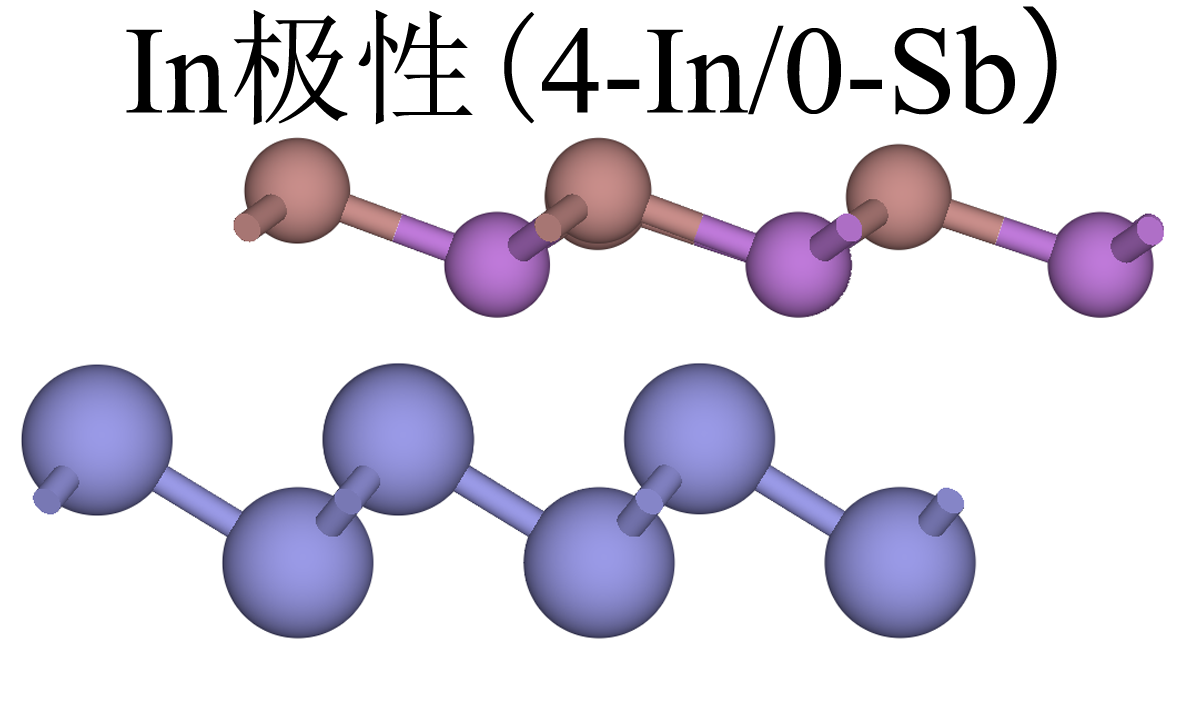
\includegraphics[width=0.27\textwidth]{pic/IS_structure_1Linsb_40side.png} \\[-0.5ex]
            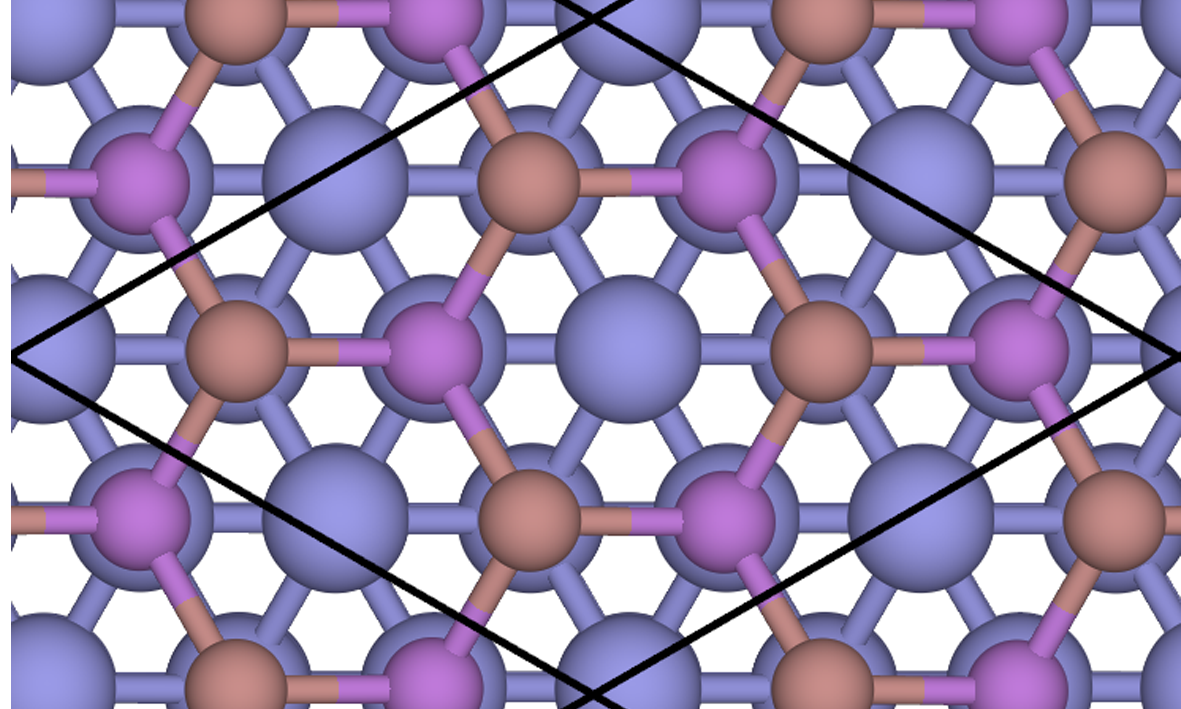
\includegraphics[width=0.27\textwidth]{pic/IS_structure_1Linsb_40top.png}
        \end{tabular}
    }
    \caption{\cemb{Bi(001)}衬底上不同极性单层\cemb{InSb}的原子结构。原子结构图中,\cemb{Bi}原子使用蓝色表示,\cemb{In}原子使用褐色表示,\cemb{Sb}原子使用紫色表示}
    \label{fig:IS_structure_1Linsb_allPolarity}
\end{figure}

这里,本文使用\cemb{InSb}单层中处于$\TfourSite$的原子的数量来表示不同极性的\cemb{InSb(111)}单层,例如在$2 \times 2$切片模型中理想的\cemb{In}极性\cemb{InSb}中,四个$\TfourSite$都被\cemb{In}原子占据,因此可以表示为\InSbMLpolar{4}{0}。相对应的,\cemb{Sb}极性的\cemb{InSb}可以表示为\InSbMLpolar{0}{4}。对于\InSbMLpolar{2}{2}极性的\cemb{InSb}单层,有两个不等价的构型。其中一个构型内部\cemb{In}原子和\cemb{Sb}分别构成两个相互嵌套的方形的四个顶角,用\InSbMLpolar{2}{2}方形表示。另一个构型中\cemb{In}原子和\cemb{Sb}原子呈条状分布,用\InSbMLpolar{2}{2}条形表示。

如图\ref{fig:IS_DFT_1LInSb_all}所示,本文计算了所有极性的$2 \times 2 \cemb{InSb}$在\cemb{Bi(001)}衬底表面的形成能。在$2 \times 2$模型中,\cemb{In}极性(\InSbMLpolar{4}{0})的形成能为\SI{-18.52}{\mievpas},低于$2 \times 2$模型中\cemb{Sb}极性(\InSbMLpolar{0}{4})的形成能(\SI{-14.64}{\mievpas})。$2 \times 2 \cemb{InSb}$理想极性(\cemb{Sb}极性和\cemb{In}极性)的计算结果与上一节中$1 \times 1$模型一致。$2 \times 2$模型中更低的形成能可能是由于表面原子在$2 \times 2$模型中有更多的空间可以进行更完全的几何优化。

\begin{figure}[htb]
    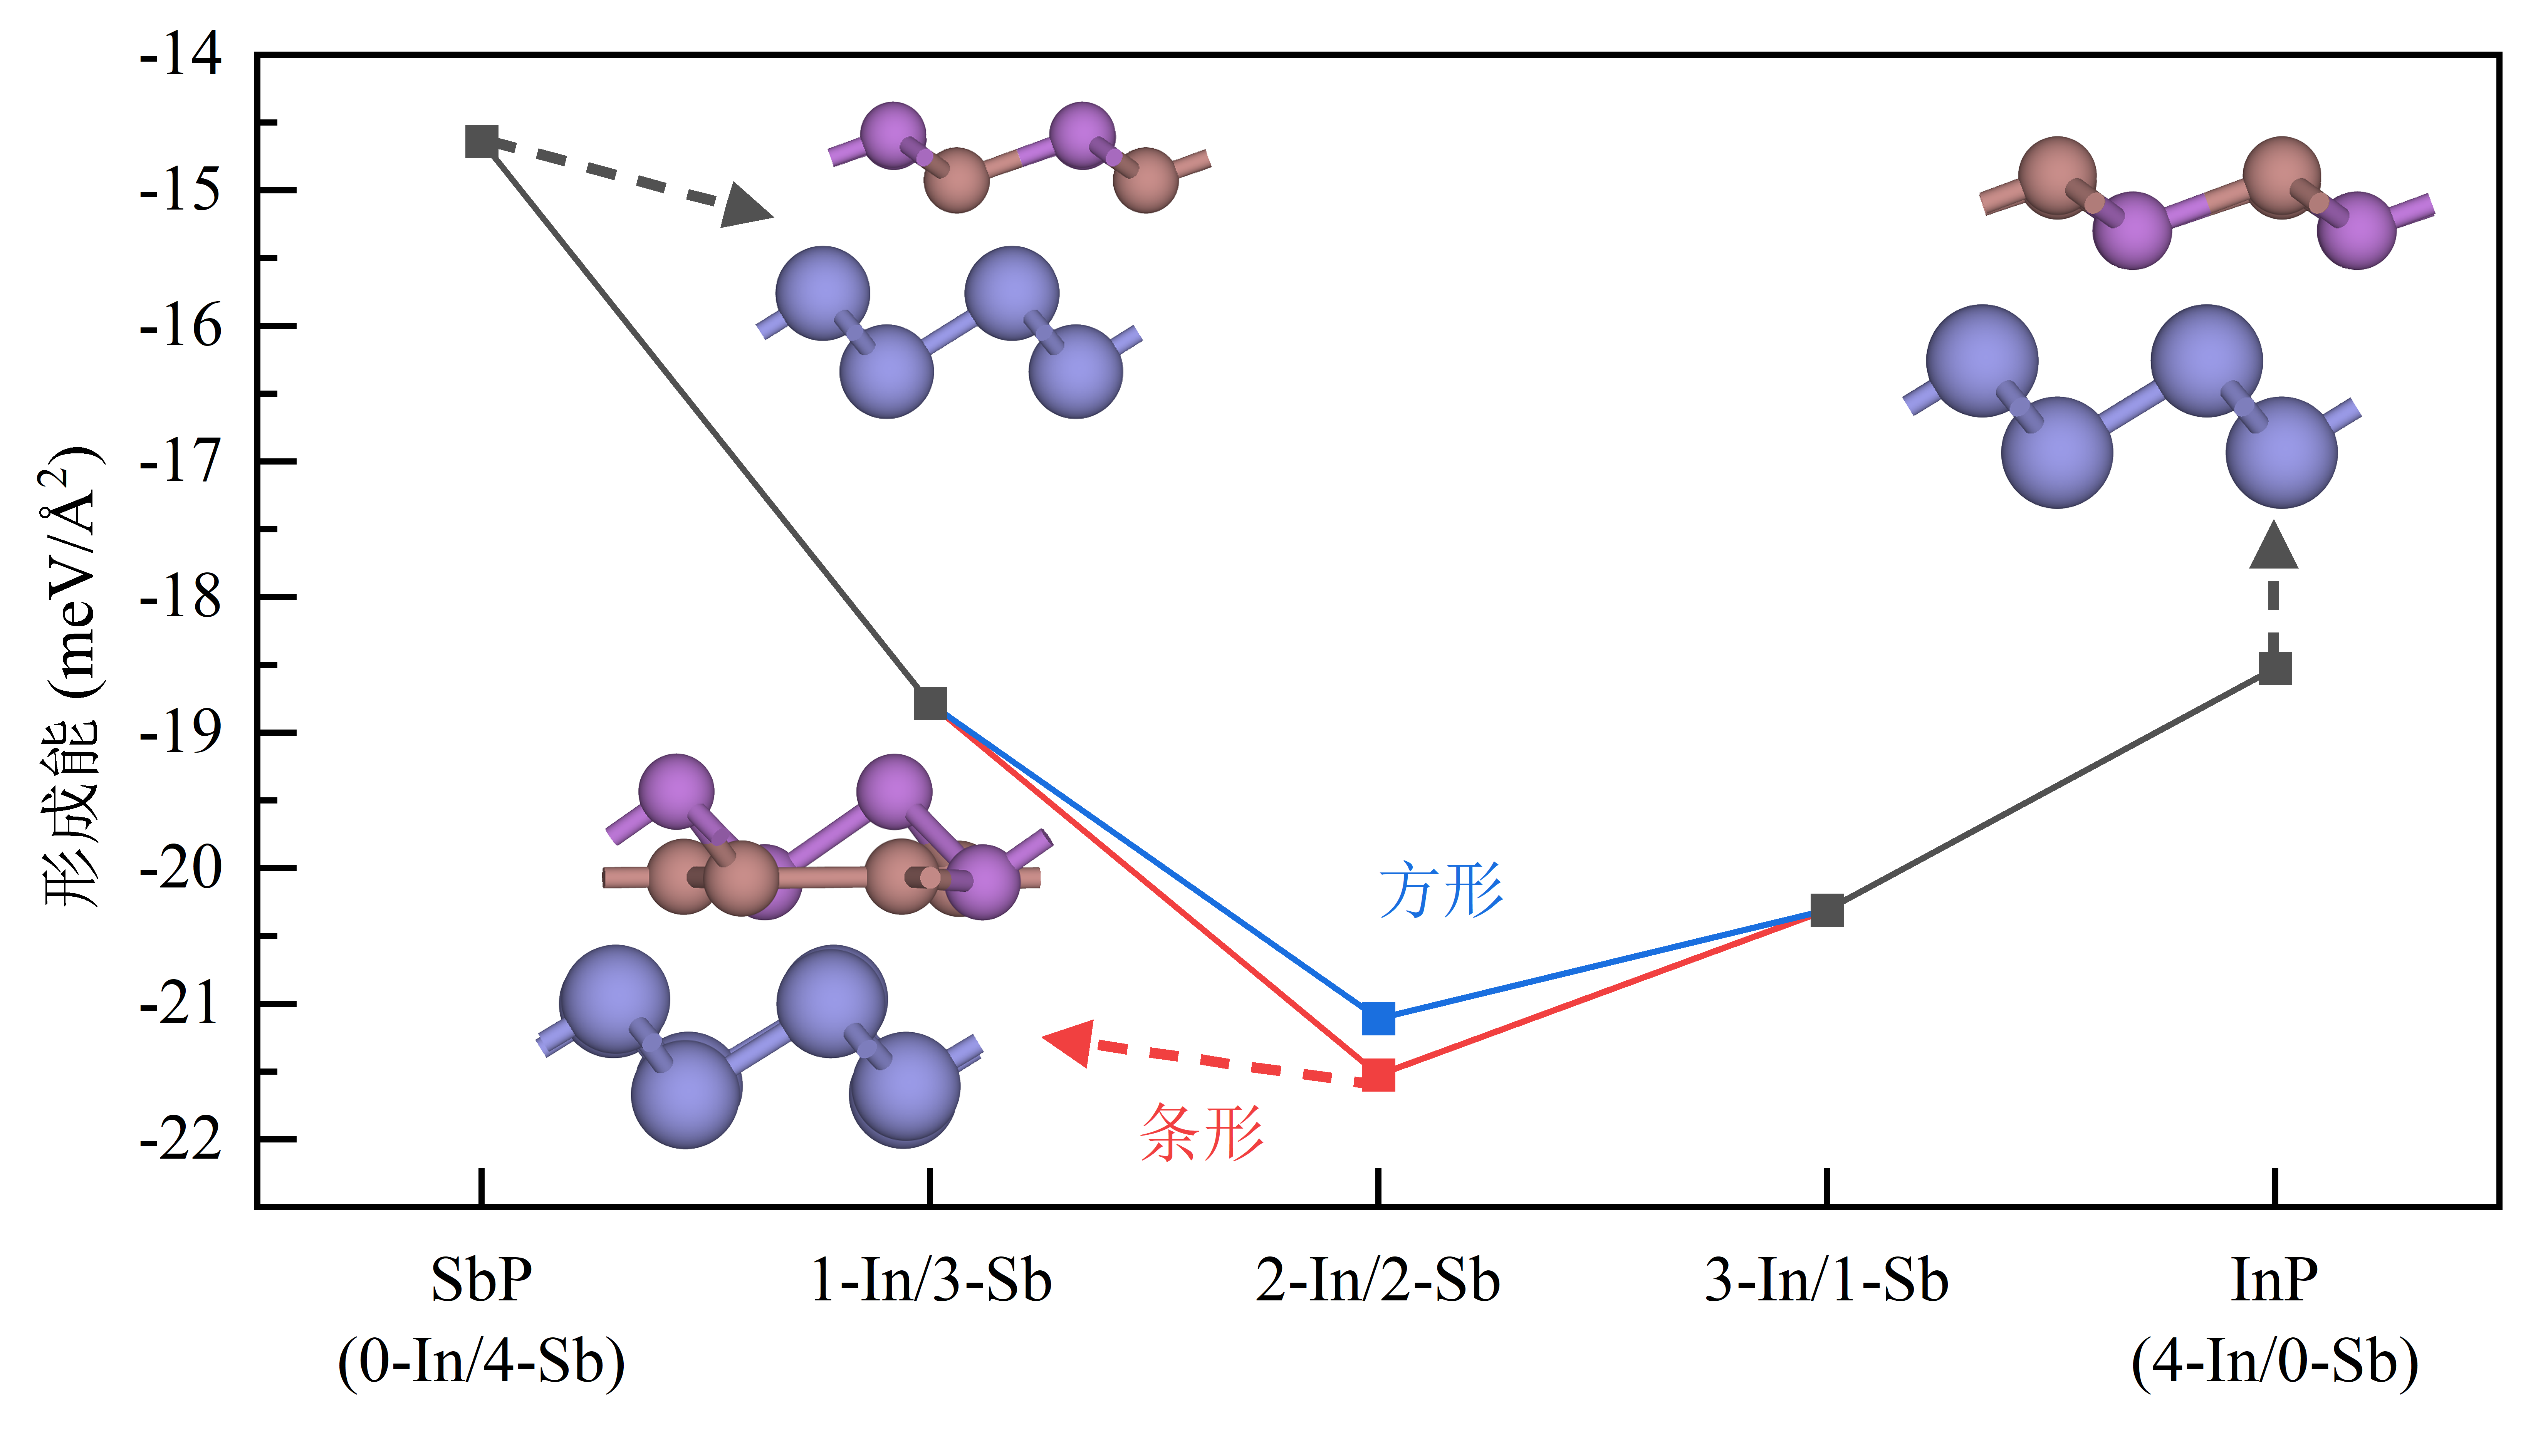
\includegraphics{pic/IS_DFT_1LInSb_all.png}
    \caption{\cemb{Bi(001)}衬底上不同极性单层\cemb{InSb}的形成能}
    \label{fig:IS_DFT_1LInSb_all}
\end{figure}

在本文的进一步计算中,本文发现混合极性的单层\cemb{InSb(111)}构型(\InSbMLpolar{1}{3}、\InSbMLpolar{2}{2}以及\InSbMLpolar{3}{1})在形成能上更具有优势。从图\ref{fig:IS_DFT_1LInSb_all}上可以看出,混合极性中能量最低的\InSbMLpolar{1}{3}构型的形成能也略低于理想极性中更为稳定的\cemb{In}极性(\InSbMLpolar{4}{0})。因此,由于混合极性具有更高的能量稳定性,在生长的过程中\cemb{InSb}单层会倾向于由理想极性的结构(\cemb{Sb}极性和\cemb{In}极性)转变为混合极性。在4种混合极性中\InSbMLpolar{2}{2}结构的单层\cemb{InSb}的形成能最低。其中,\InSbMLpolar{2}{2} 条形构型的形成能略低与\InSbMLpolar{2}{2}方形构型的形成能。这两形成能相近的\InSbMLpolar{2}{2}构型形成的能量最低态使得混合极性的\cemb{InSb}单层倾向于较为均匀的分布于这两个\InSbMLpolar{2}{2}构型之中,形成类似于非晶态的\cemb{InSb}单层。

利用分子动力学模拟方法,本文测试了\InSbMLpolar{2}{2}构型的热稳定性。如图\ref{fig:IS_structure_1Linsb_md}所示,选用形成能更低的\InSbMLpolar{2}{2} 条形构型作为考察对象(图\ref{fig:IS_structure_1Linsb_md0ps}),模拟温度设为生长\cemb{InSb}常见的\SI{400}{\kelvin}。可能看到,在经过\SI{30}{\pico\second}的分子动力学模拟后。\cemb{InSb}单层的晶格结构被略微破坏,其中\cemb{In}的条状构型已经被热动能破坏,形成类似于菱形的结构,而\cemb{Sb}的条状构型保持较为完好。综合以上的计算结果,本文认为\cemb{InSb(111)}单层在\cemb{Sb(001)}衬底上由于热涨落的作用很可能无法保持在唯一的构型下,而是处于不同混合极性的热平衡态。在热平衡中,不同极性的\cemb{InSb}在热动能的驱动下相互转化,形成非晶态的单层\cemb{InSb}形貌。

\begin{figure}[htb]
    \subfloat[]{
        \label{fig:IS_structure_1Linsb_md0ps}
        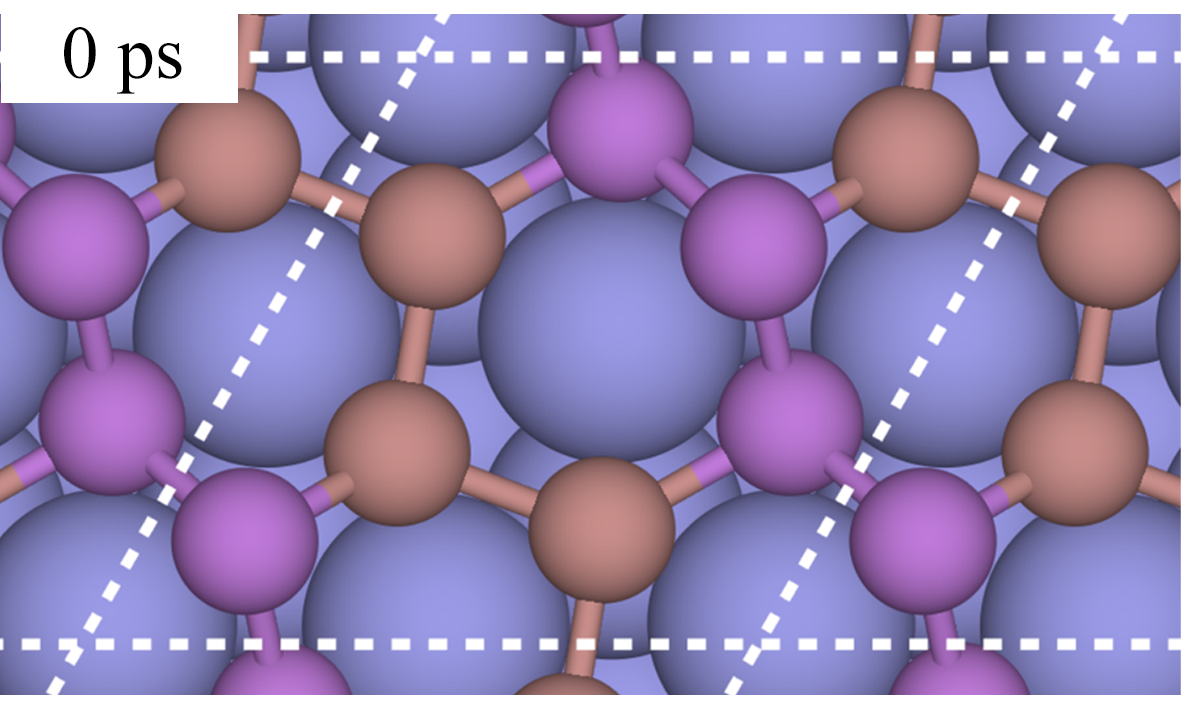
\includegraphics{pic/IS_structure_1Linsb_md0ps.png}
    }
    \subfloat[]{
        \label{fig:IS_structure_1Linsb_md10ps}
        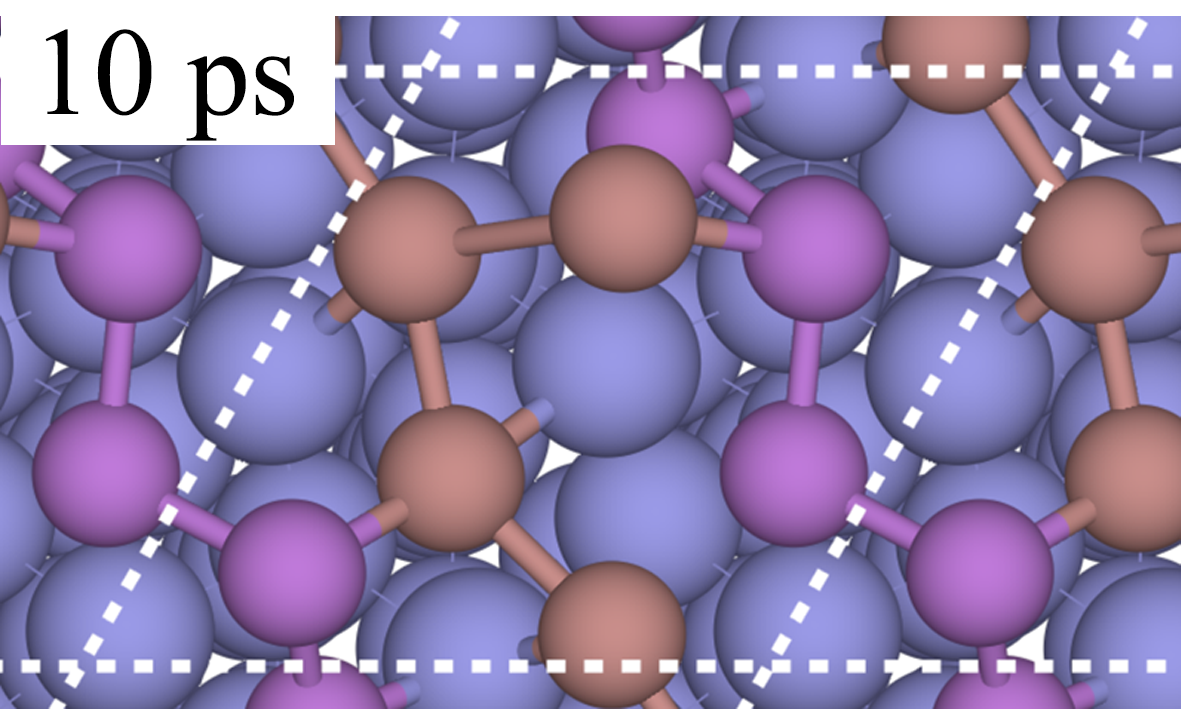
\includegraphics{pic/IS_structure_1Linsb_md10ps.png}
    }\\[-1ex]
    \subfloat[]{
        \label{fig:IS_structure_1Linsb_md20ps}
        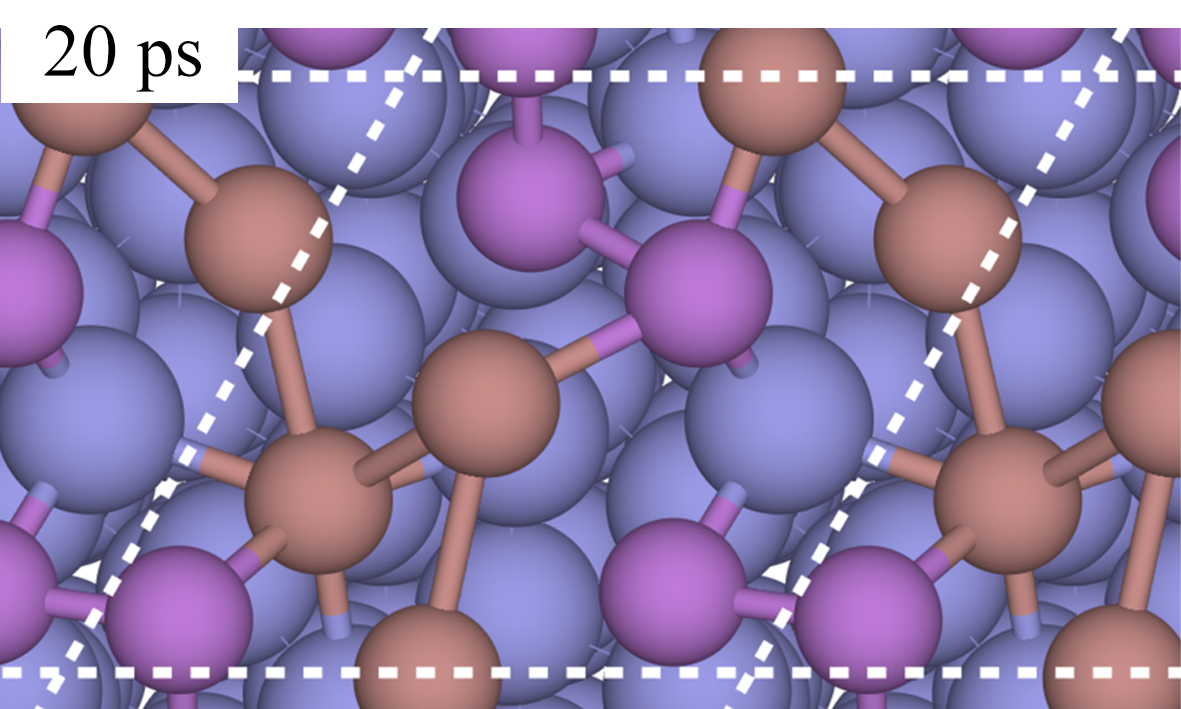
\includegraphics{pic/IS_structure_1Linsb_md20ps.png}
    }
    \subfloat[]{
        \label{fig:IS_structure_1Linsb_md30ps}
        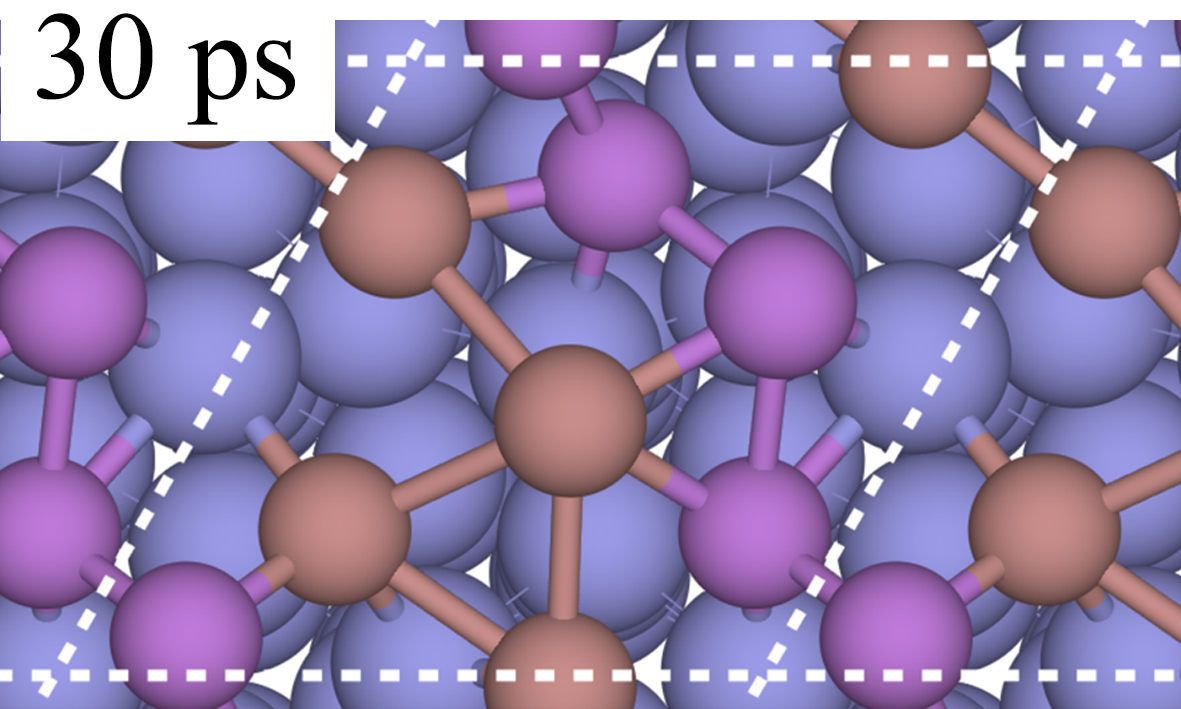
\includegraphics{pic/IS_structure_1Linsb_md30ps.png}
    }
    \caption{\cemb{Bi(001)}衬底上2-In/2-Sb条形极性\cemb{InSb}的分子动力学模拟结果。原子结构图中,\cemb{Bi}原子使用蓝色表示,\cemb{In}原子使用褐色表示,\cemb{Sb}原子使用紫色表示}
    \label{fig:IS_structure_1Linsb_md}
\end{figure}

对于单层\cemb{InSb(111)}不同极性之间的转换能力,本文通过将单层\cemb{InSb(111)}由一个极性的构型转变为另一个极性的构型所需的势垒进行判定。取\cemb{Sb}极性和\cemb{In}极性的\cemb{InSb}单层之间的转换作为代表。这两个极性之间的转变涉及\cemb{InSb}单层内部所有的\cemb{In}原子和\cemb{Sb}原子,因此本文将其作为\cemb{InSb}极性转换势垒的上界。过渡态的计算结果如图\ref{fig:IS_DFT_1LInSb_InPtoSbPNeb}所示,从能量更高的\cemb{Sb}极性结构转变到\cemb{In}极性,单层\cemb{InSb}需要跨越约\SI{0.60}{\electronvolt}的势垒。根据统计力学原理\citing{RN945-1935},单层\cemb{InSb}从\cemb{Sb}极性转变到\cemb{In}极性的频率$r$为\chinesecolon
\[
    r=e^{\frac{-\energyVar{a}{}}{\kbconst T}}e^{\frac{\rm{\Delta} \it S}{\kbconst}} \frac{\kbconst T}{h}
\]
其中,$\energyVar{a}{}$为反应的激活能,$\kbconst$为玻尔兹曼常数,$T$为温度,$h$为普朗克常数,$\rm{\Delta} \it S$为反应过程中初态和过渡态之间的熵变,本文使用密度泛函理论计算结合原子震动能谱分析进行计算。在\SI{400}{\kelvin}的温度下,单层\cemb{InSb}从\cemb{Sb}极性转变到\cemb{In}极性的频率$r$约为\SI{3e5}{\per\second},证明了在\cemb{Bi(001)}衬底表面,\cemb{InSb}单层具有较高的极性转变能力。


\begin{figure}[htb]
    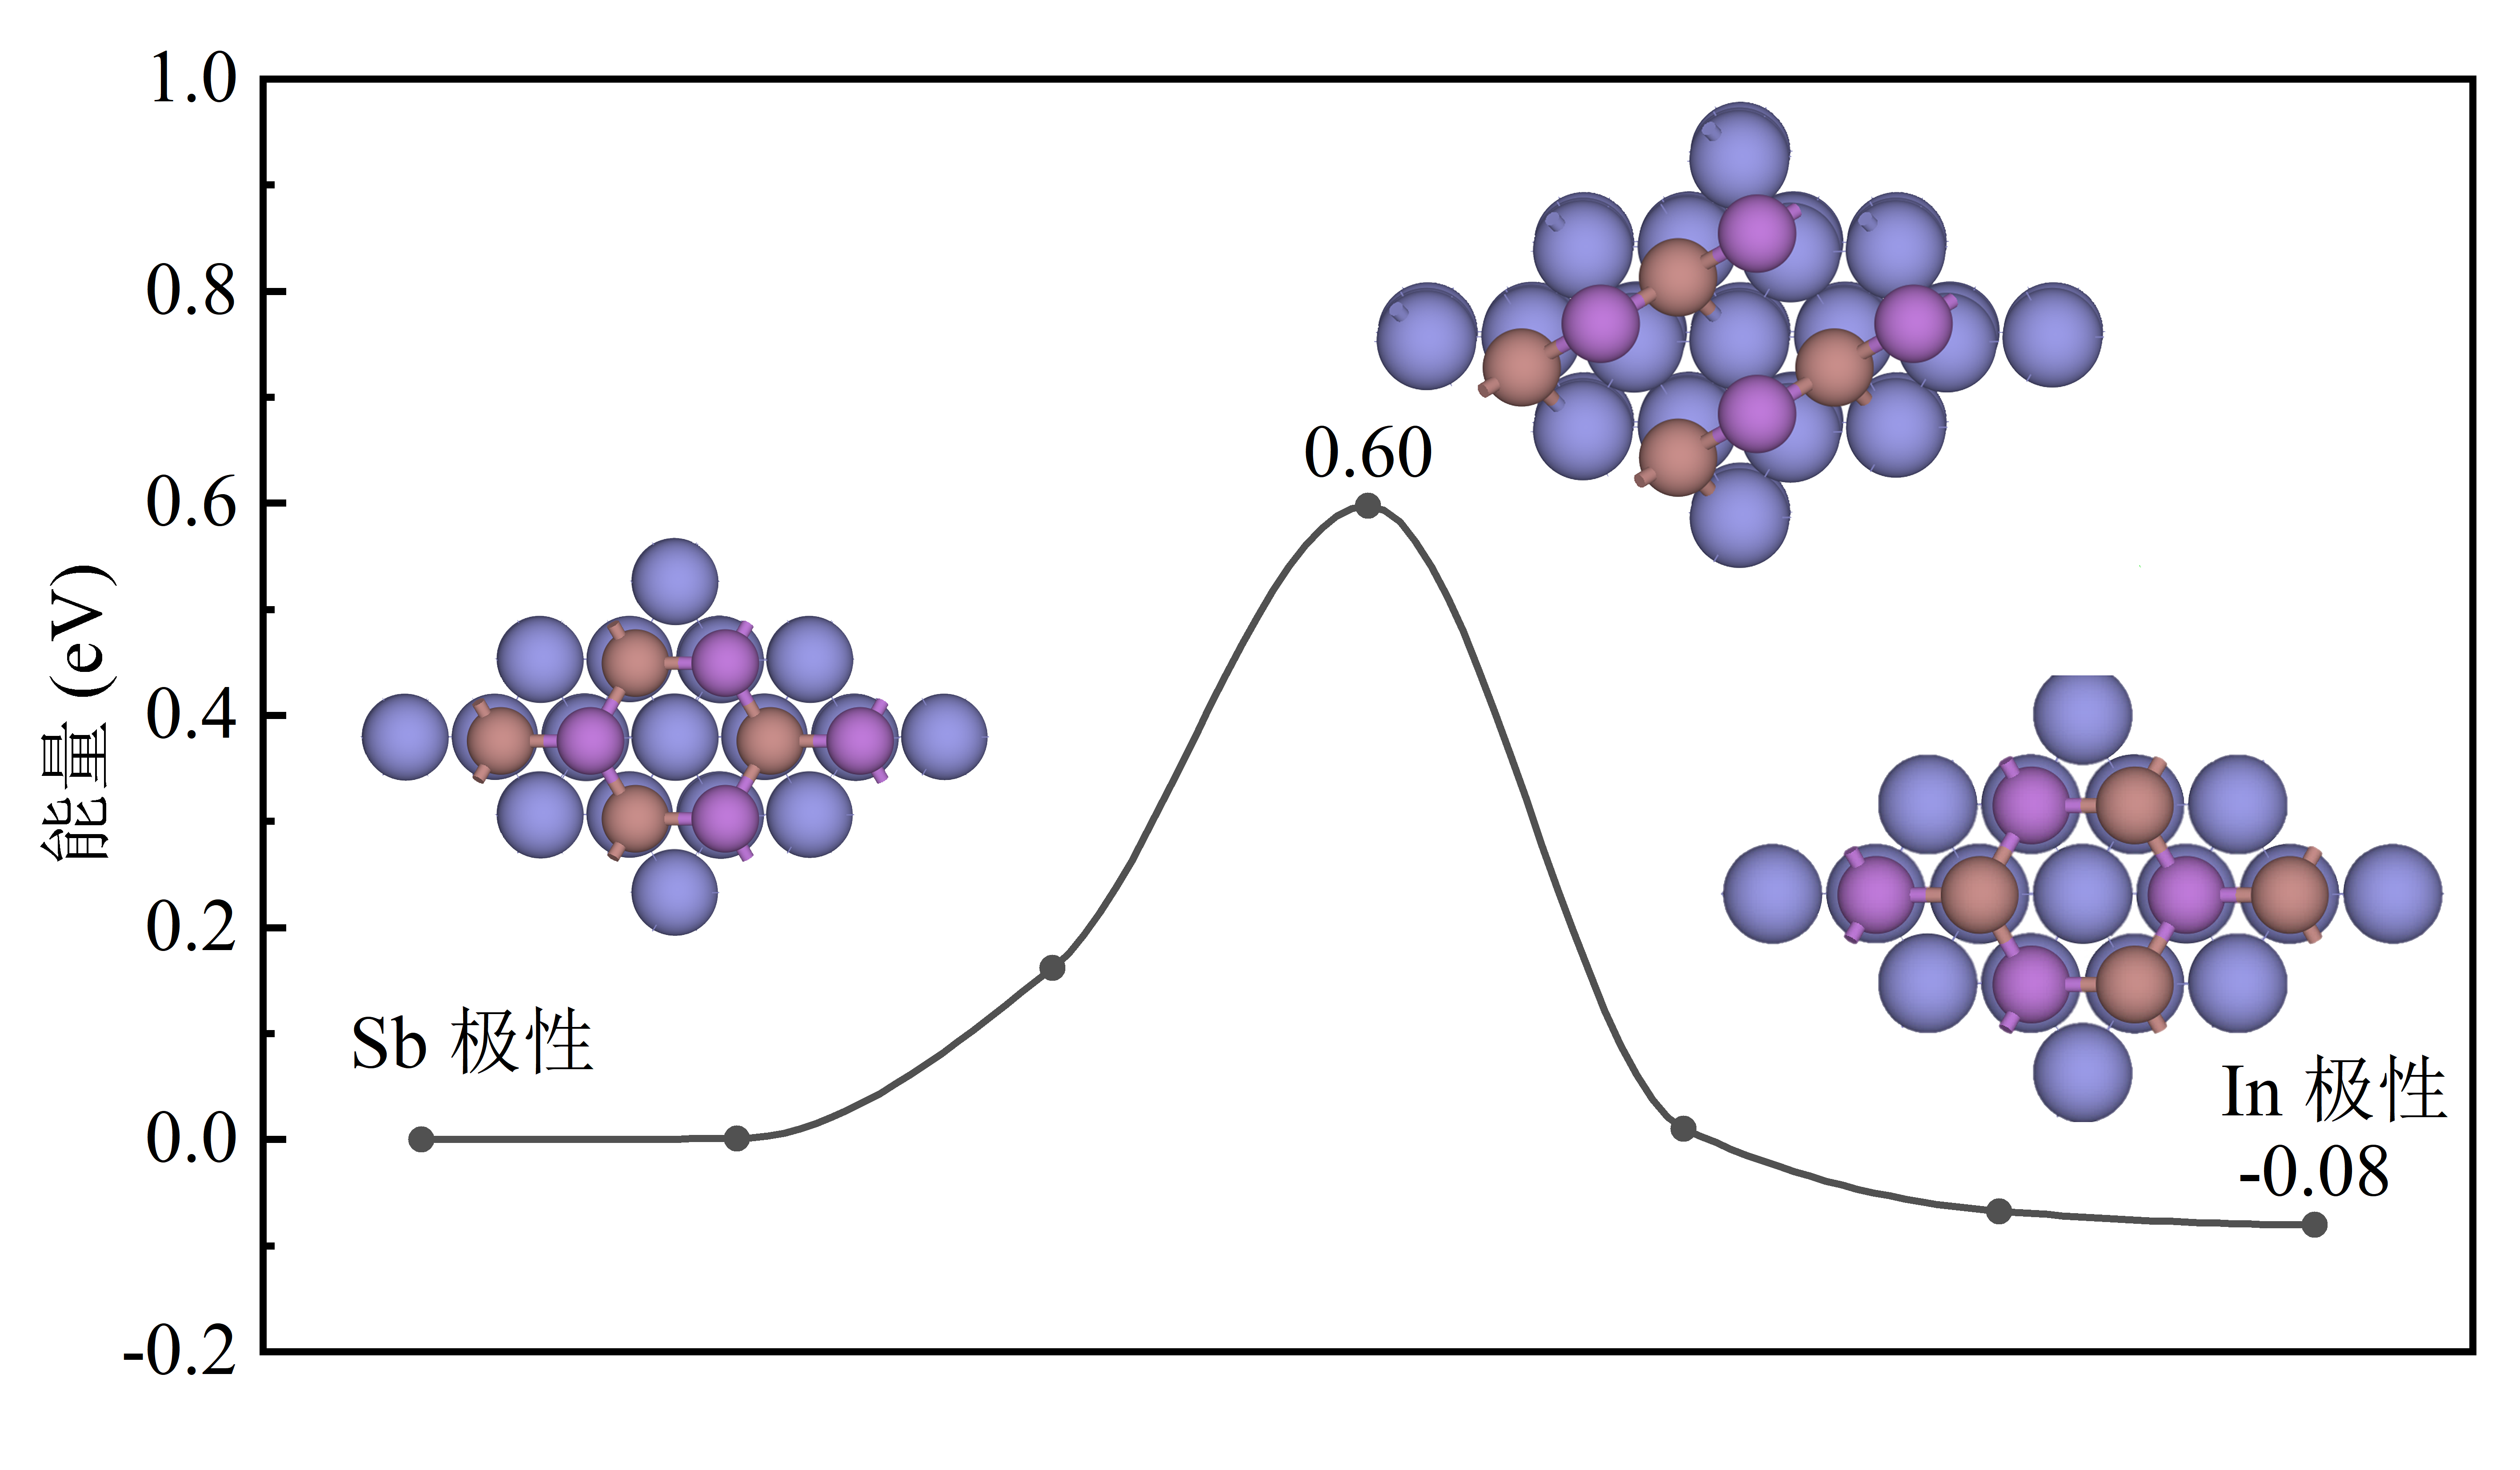
\includegraphics{pic/IS_DFT_1InSb_flipBarrier.png}
    \caption{\cemb{Bi(001)}衬底上单层\cemb{InSb}的极性转换势垒。原子结构图中,\cemb{Bi}原子使用蓝色表示,\cemb{In}原子使用褐色表示,\cemb{Sb}原子使用紫色表示}
    \label{fig:IS_DFT_1LInSb_InPtoSbPNeb}
\end{figure}

\section{双层\cemb{InSb}的生长机理}
在上一节中,本文通过理论计算表明了单层的\cemb{InS(111)}以\InSbMLpolar{2}{2}极性为主,多种极性热平衡混合的构型存在于\cemb{Bi(001)}衬底的表面。本文将第二层\cemb{InSb(001)}放置在单层\cemb{InSb}上方,研究双层\cemb{InSb(111)}在\cemb{Bi(001)}衬底上的生长机理和极性演化情况。

\subsection{双层\cemb{InSb}的生长过程}
\label{cap:IS_2L_growthProcess}
对于双层\cemb{InSb}在\cemb{Bi(001)}衬底上的生长,本文首先探究第二层\cemb{InSb(111)}对于\cemb{InSb}极性的影响。对于第二层\cemb{InSb(111)},本文选用对应的表面重构构型进行代表。根据先前的研究\citing{RN915-1998, RN896-1998},在\cemb{InSb(111)}的表面由于极性的不同会形成两种不同的表面重构,一种是对应于\cemb{Sb}极性的\cemb{Sb}三聚体(\cemb{Sb} trimer)表面重构,另一种是对应于\cemb{In}极性的\cemb{In}空位(\cemb{In} vacancy)表面重构。

\begin{figure}[!htb]
    \subfloat[]{
        \label{fig:IS_2LInSb_config}
        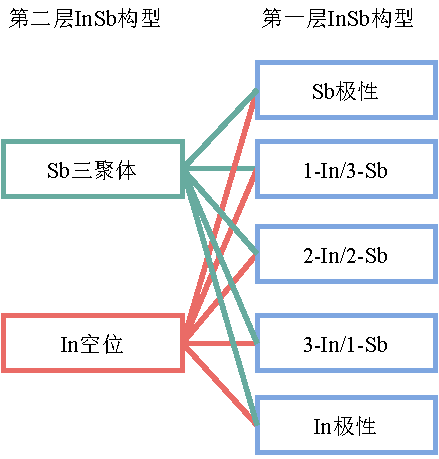
\includegraphics[width=0.48\textwidth]{pic/IS_2LInSb_config.pdf}
    }
    \begin{minipage}[b]{0.5\textwidth}
        \subfloat[]{
            \label{fig:IS_structure_2Linsb_SbT40}
            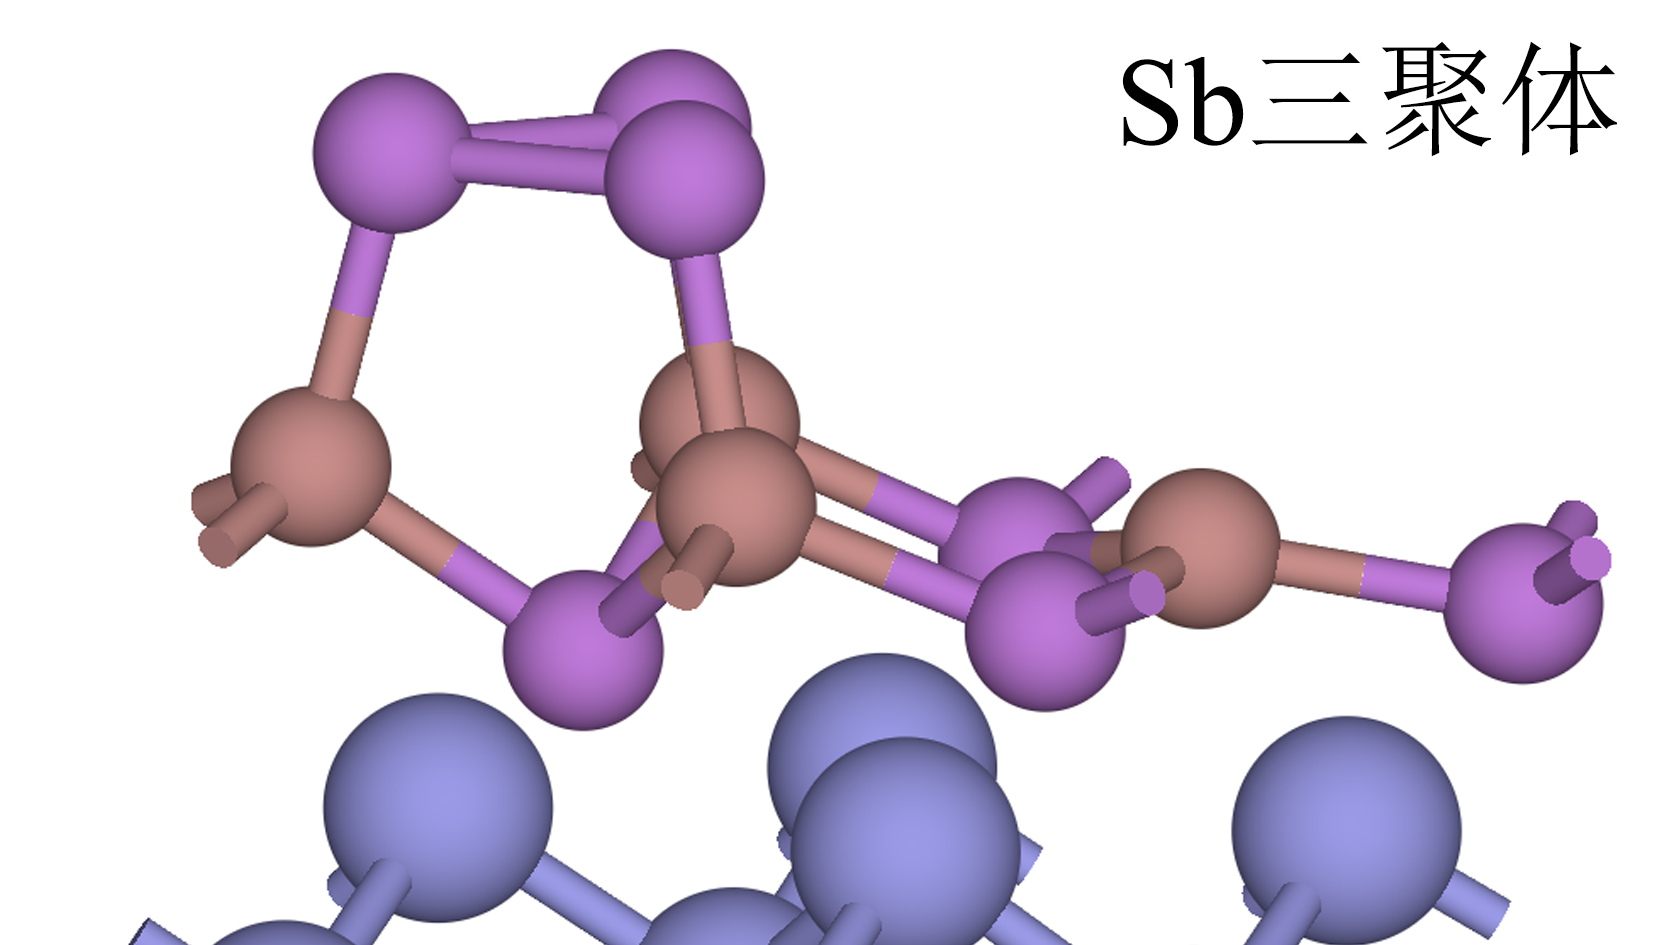
\includegraphics[width=0.8\textwidth]{pic/IS_structure_2Linsb_SbT-40_3Dview.png}
        }
        \newline
        \subfloat[]{
            \label{fig:IS_structure_2Linsb_InV40}
            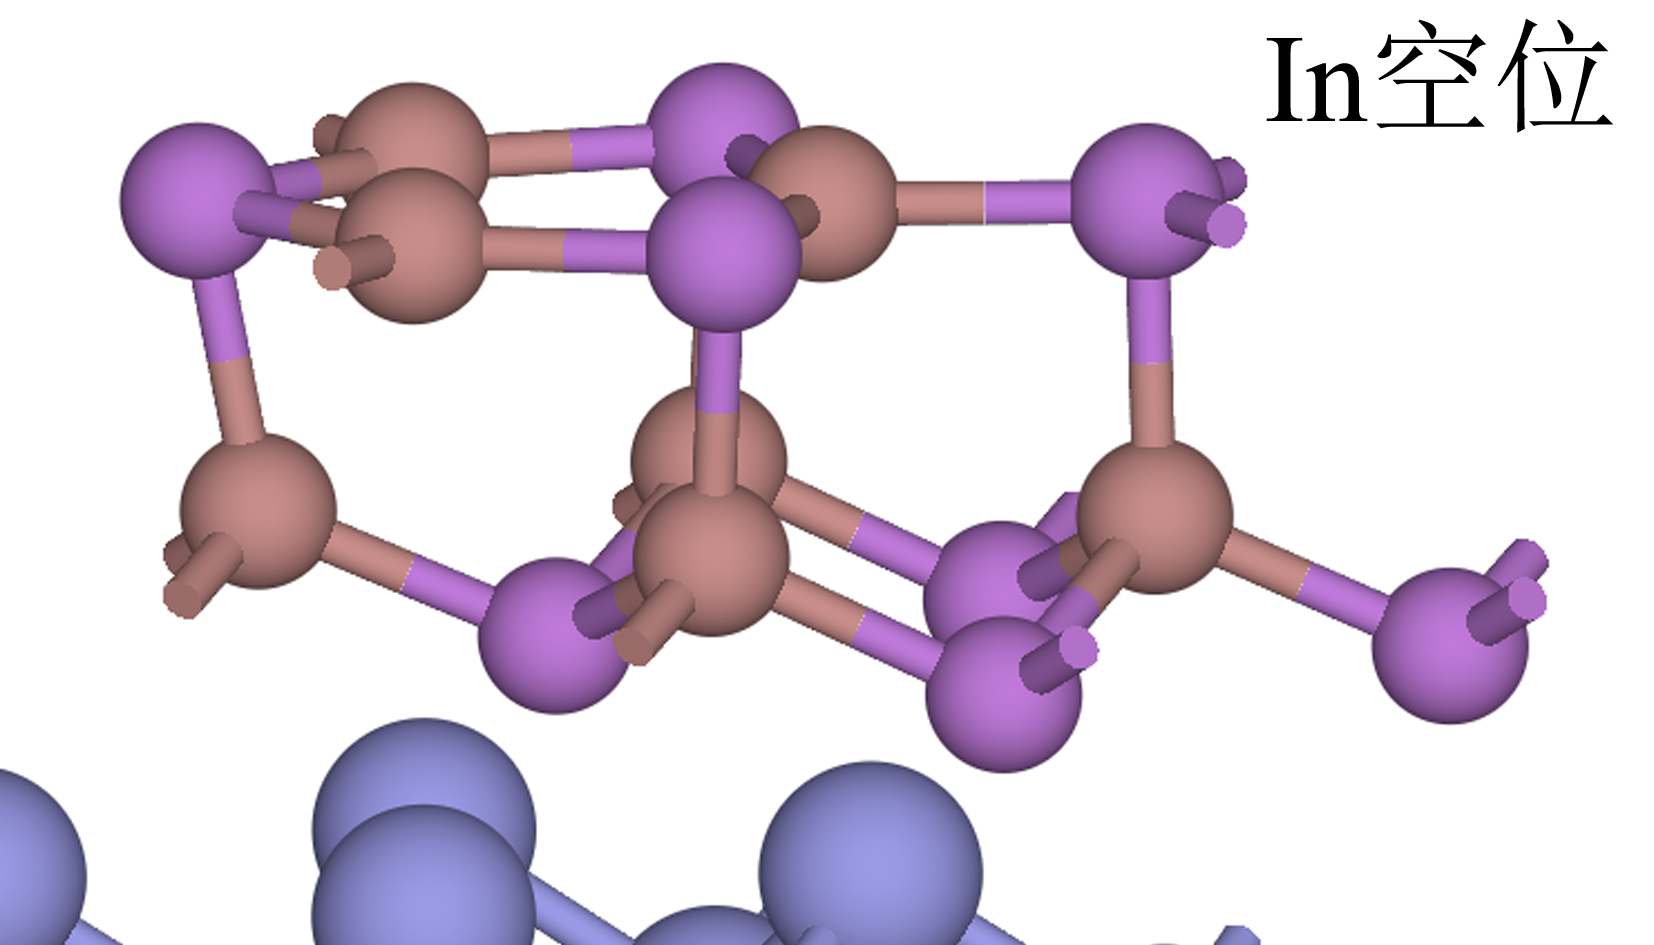
\includegraphics[width=0.8\textwidth]{pic/IS_structure_2Linsb_InV-40_3Dview.png}
        }
    \end{minipage}
    \caption{双层\cemb{InSb}极性极性组合图及原子结构示意图。(a)双层\cemb{InSb}极性极性组合示意图;(b)双层\cemb{InSb}原子结构,\cemb{Sb}三聚体第二层覆盖\cemb{In}极性第一层;(b)双层\cemb{InSb}原子结构,\cemb{In}空位第二层覆盖\cemb{In}极性第一层。原子结构图中,\cemb{Bi}原子使用蓝色表示,\cemb{In}原子使用褐色表示,\cemb{Sb}原子使用紫色表示}
    \label{fig:IS_structure_2Linsb}
\end{figure}

如图\ref{fig:IS_structure_2Linsb}所示,本文考虑不同表面重构的\cemb{InSb}第二层和不同极性的\cemb{InSb}第一层的所有组合进行形成能计算。以\cemb{In}极性的\cemb{InSb}第一层为代表,在图\ref{fig:IS_structure_2Linsb_SbT40}和图\ref{fig:IS_structure_2Linsb_InV40}中绘制了优化后的双层\cemb{InSb}的原子结构。可以看到对于\cemb{Sb}三聚体的第二层能够与\cemb{In}极性的第一层的上表面\cemb{In}原子产生相互作用,略微提高于其相接触的\cemb{In}原子的相对高度。对于\cemb{In} 空位的第二层,其在\cemb{In}极性的第一层\cemb{InSb}上方呈现出平面化的形貌。\cemb{In}空位重构中四个\cemb{Sb}原子与第一层上表面的\cemb{In}原子产生作用。

\begin{figure}[htb]
    \subfloat[]{
        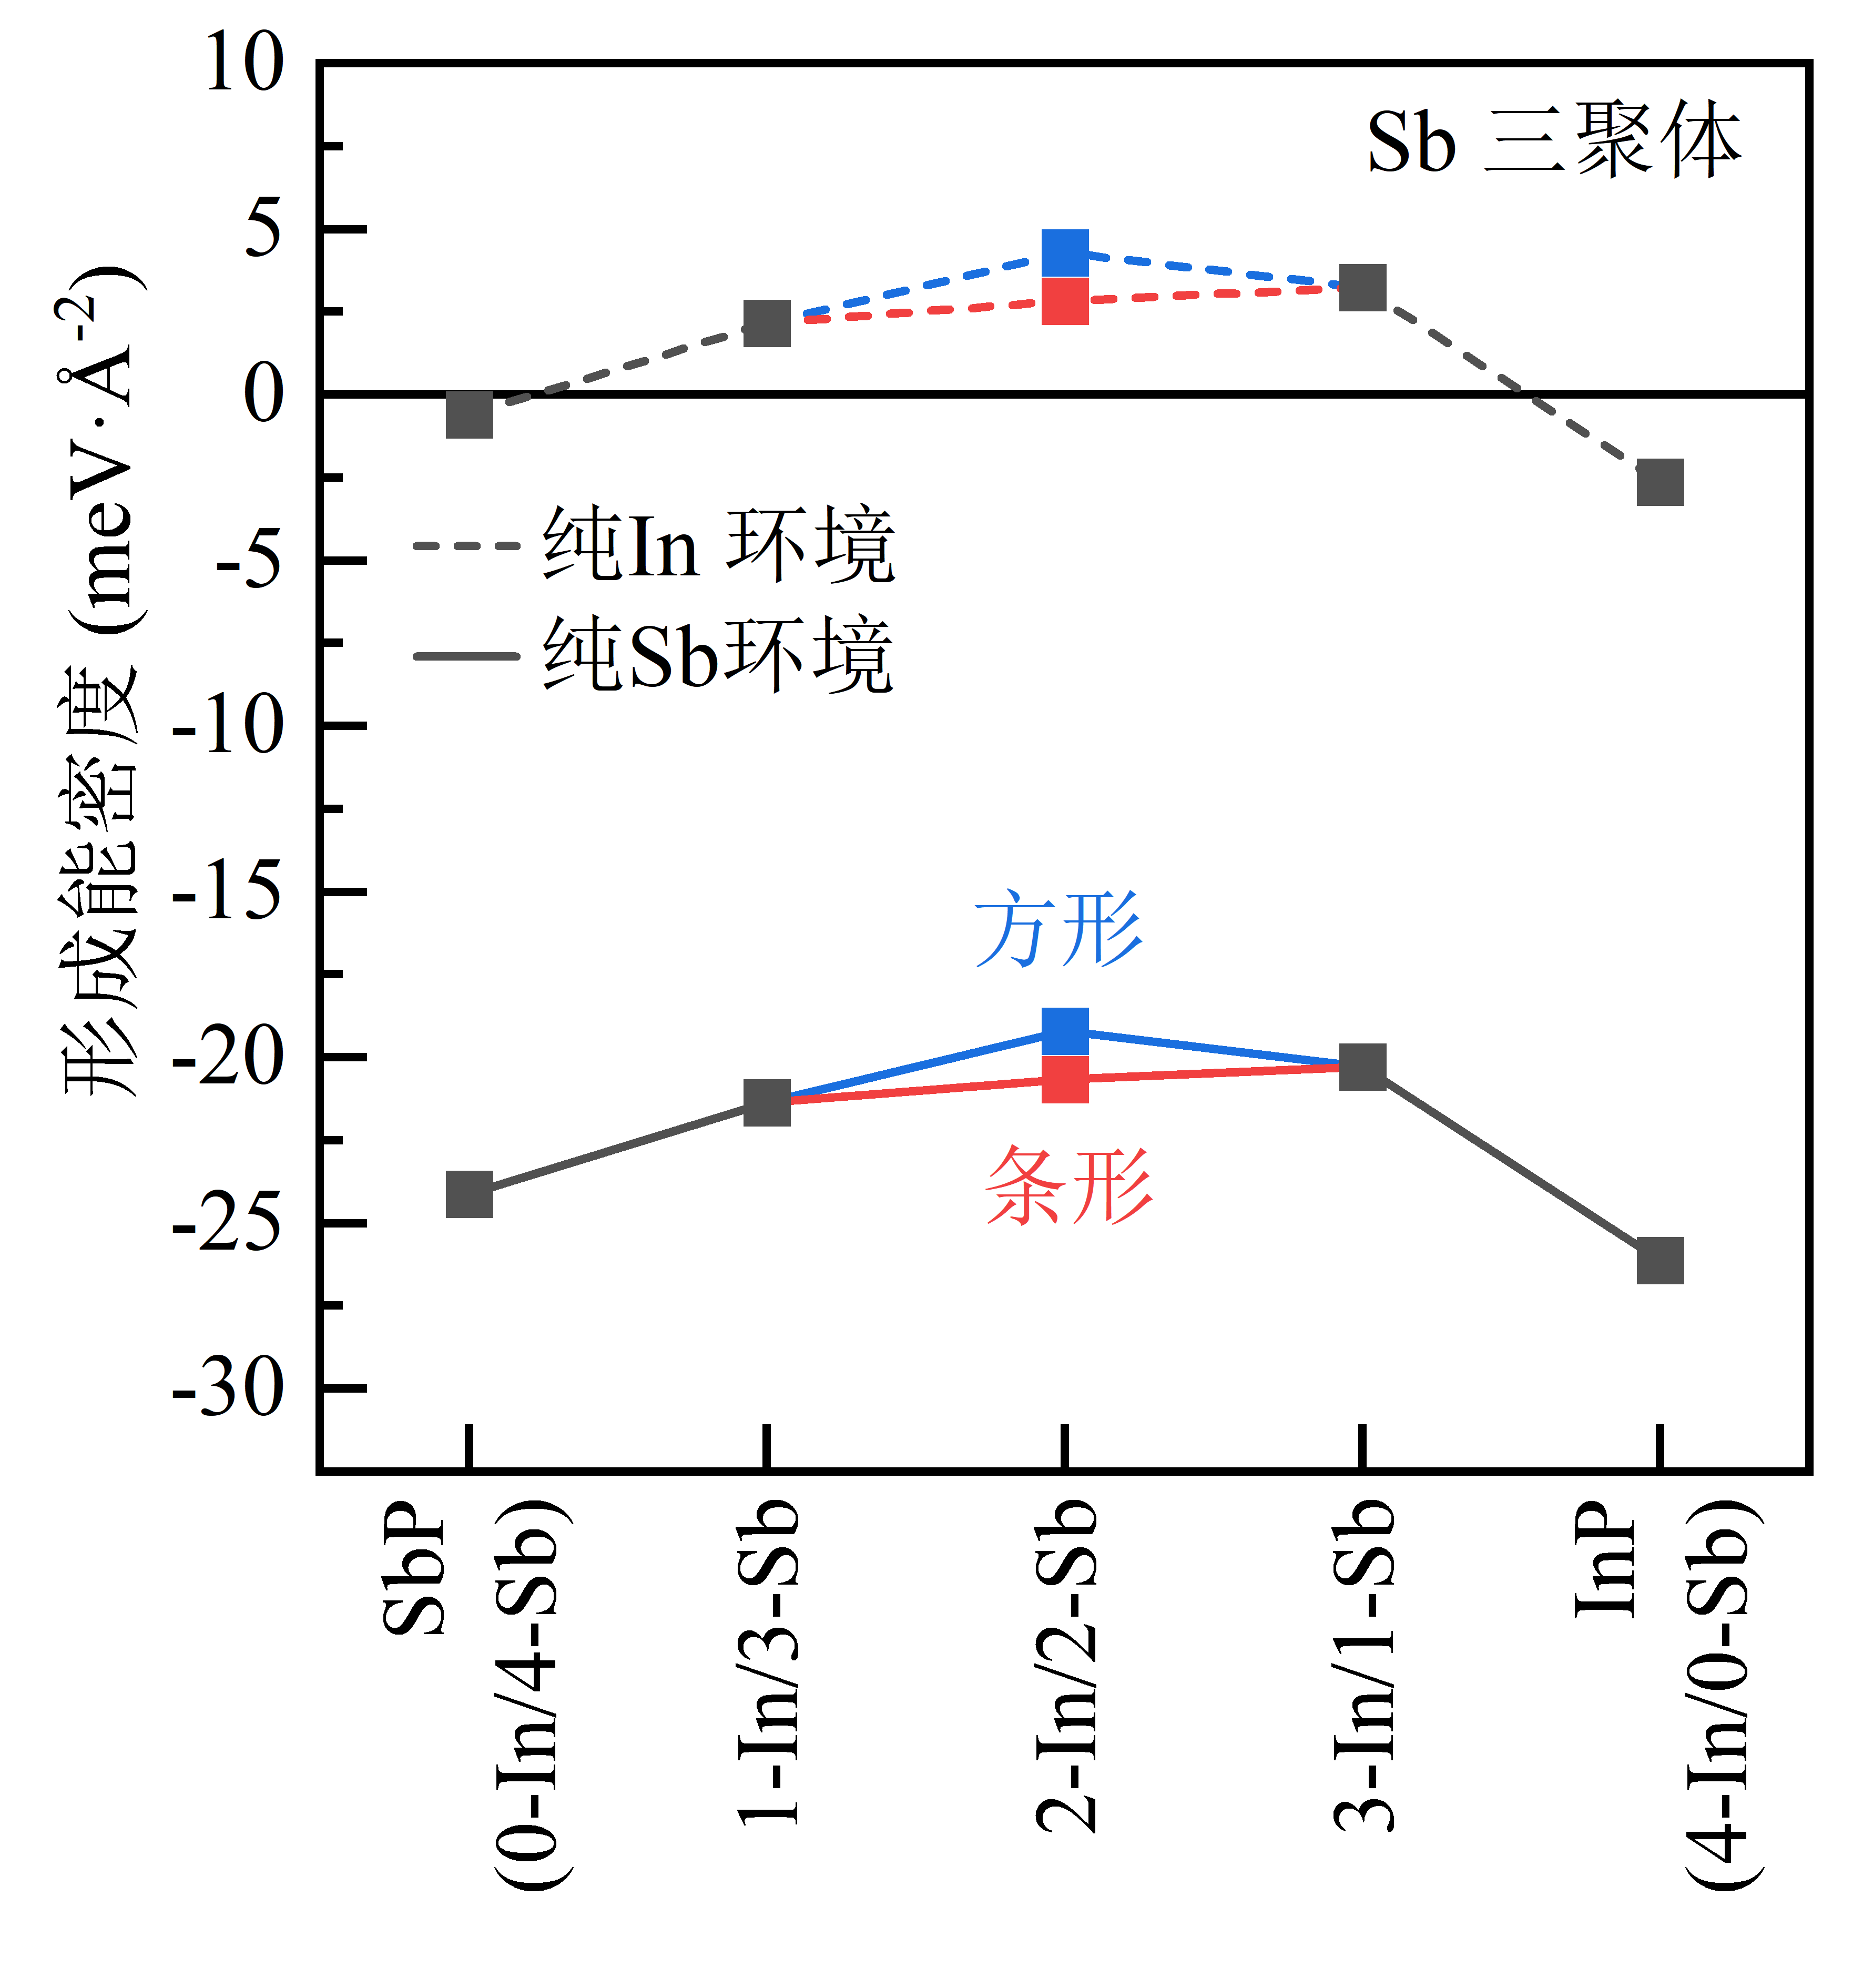
\includegraphics[width=0.45\textwidth]{pic/IS_DFT_2LInSb_SbTonAll.png}
        \label{fig:IS_DFT_2LInSb_SbTonAll}
    }
    \subfloat[]{
        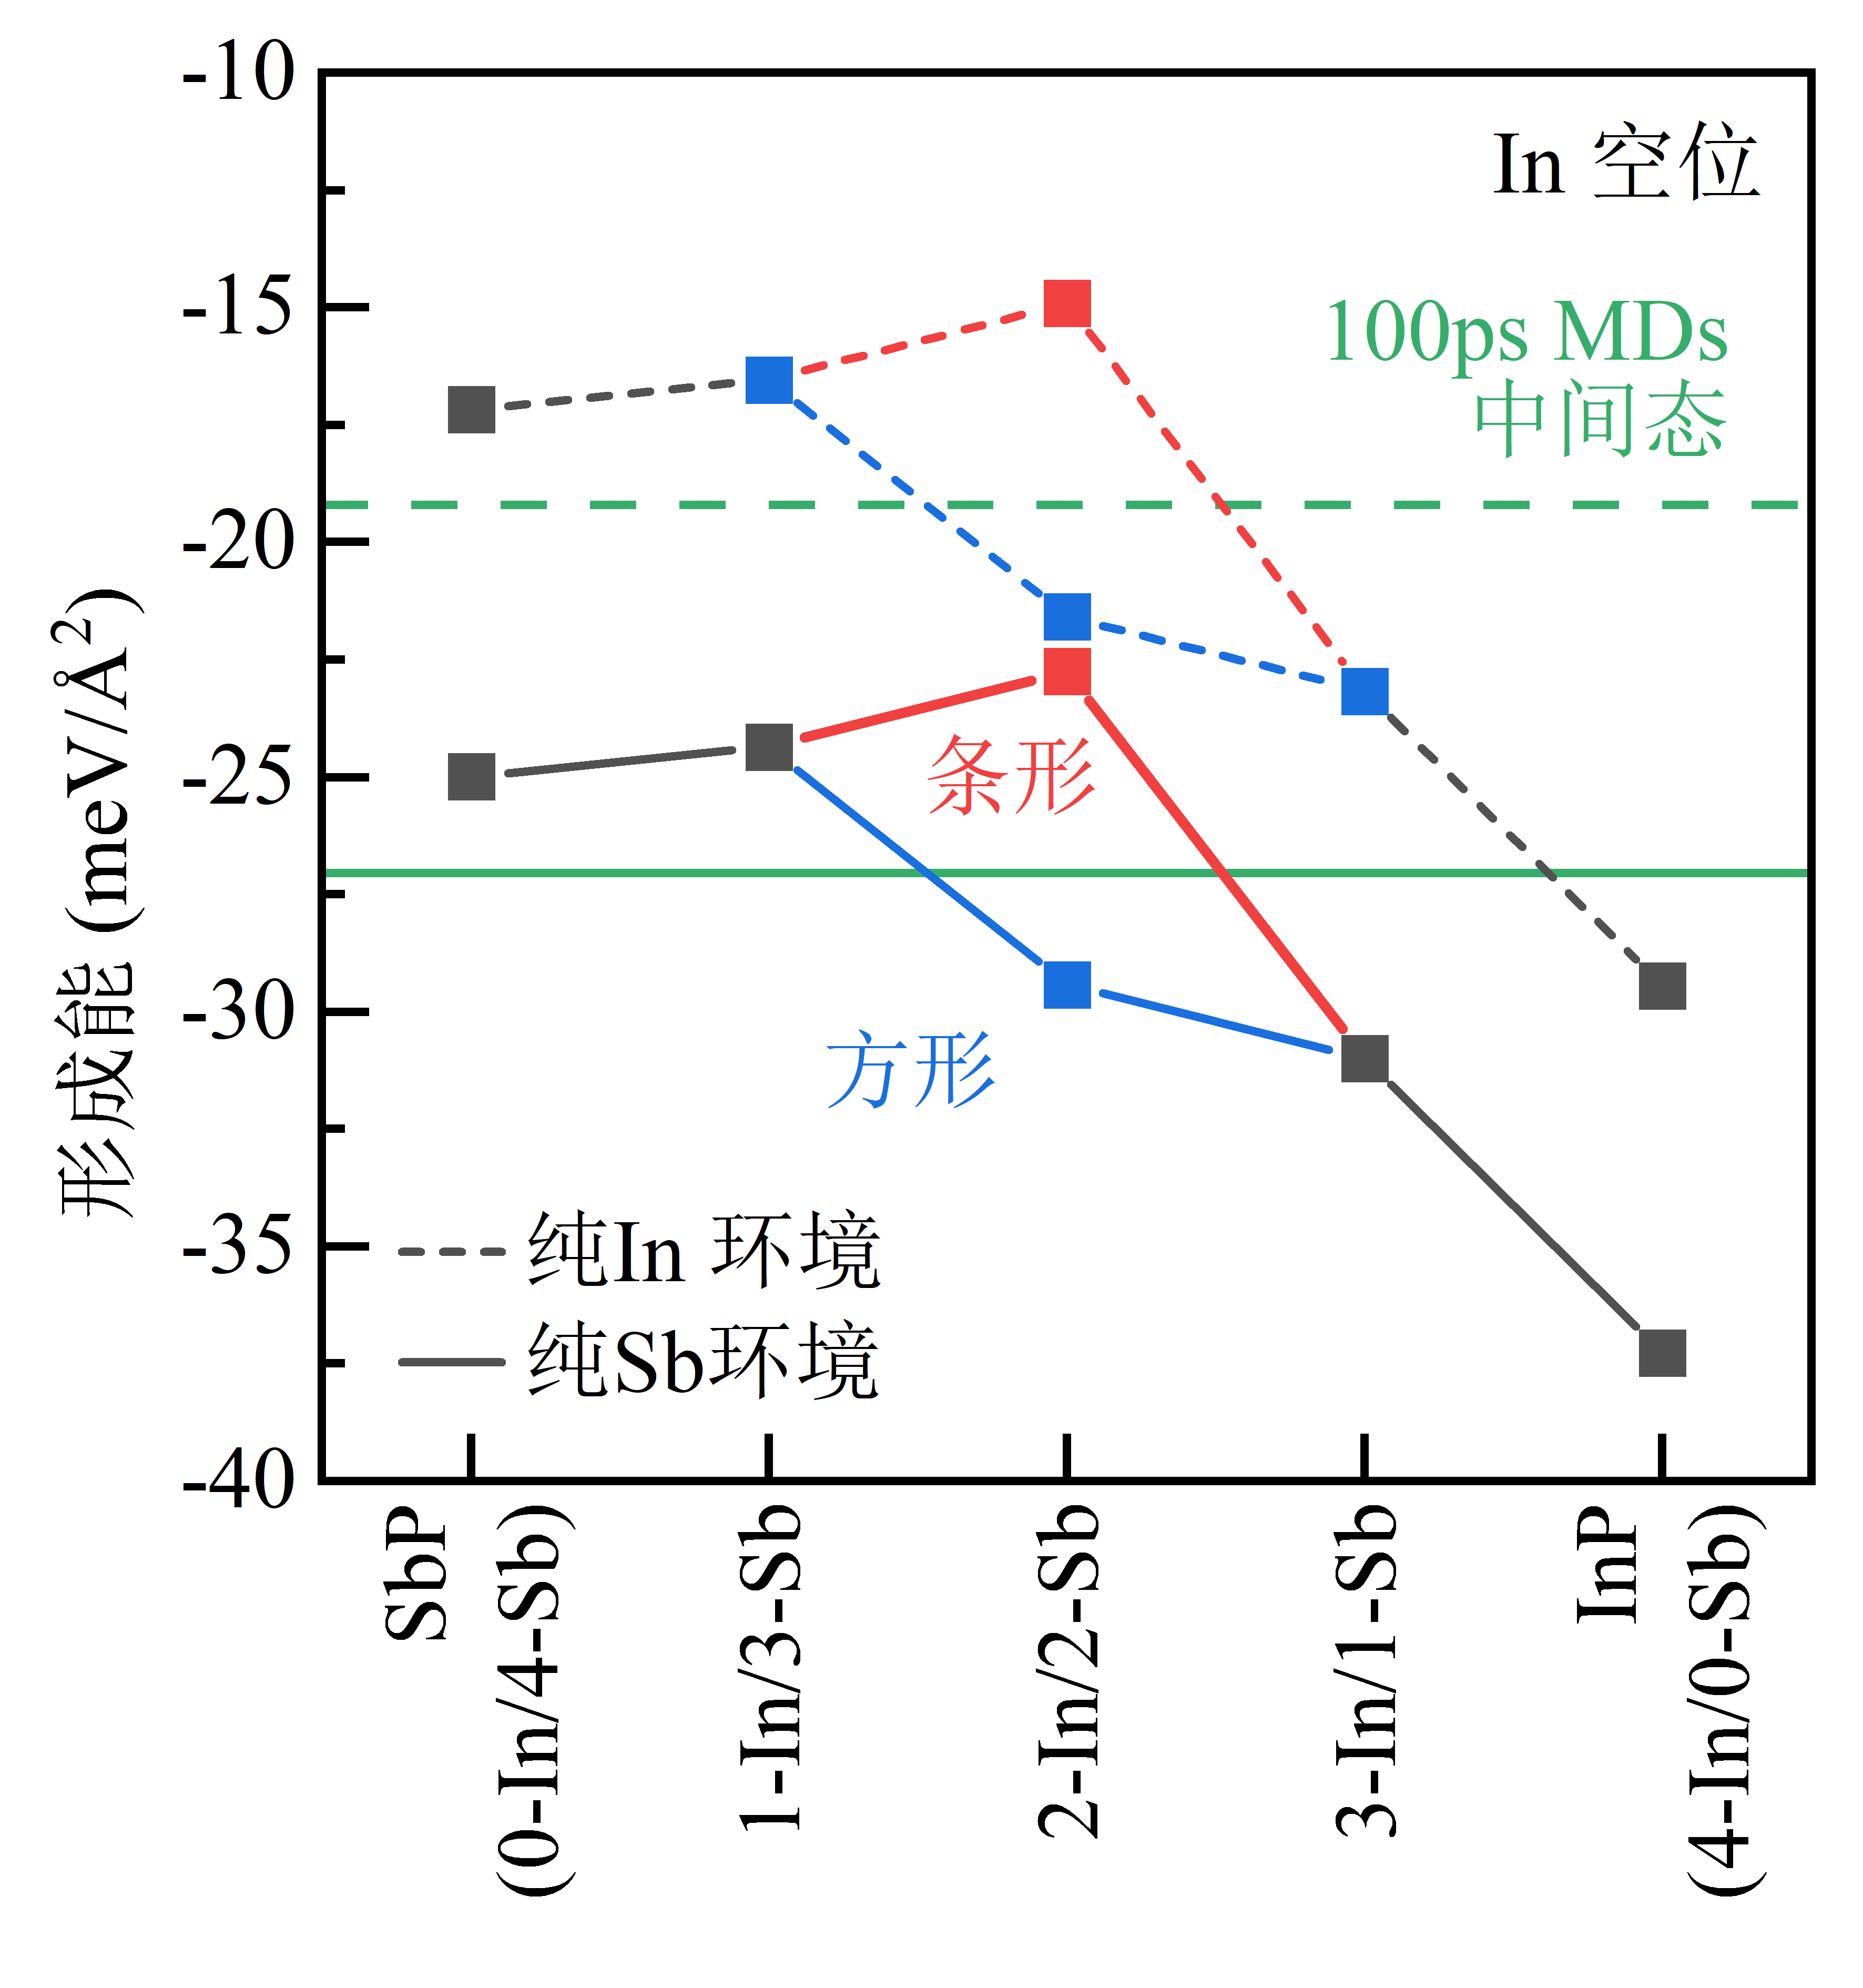
\includegraphics[width=0.45\textwidth]{pic/IS_DFT_2LInSb_InVonAll.png}
        \label{fig:IS_DFT_2LInSb_InVonAll}
    }
    \caption{\cemb{Bi(001)}衬底上双层\cemb{InSb}的形成能分布。(a)以Sb三聚体为第二层的双层\cemb{InSb}的形成能分布;(b)以In空位层为第二层的双层\cemb{InSb}的形成能分布}
    \label{fig:IS_DFT_2LInSb_formationEnergy}
\end{figure}

在图\ref{fig:IS_DFT_2LInSb_formationEnergy}中,本文绘制了\cemb{Bi(001)}衬底上具有不同极性第一层\cemb{InSb}的双层\cemb{InSb}的形成能分布。先前的研究表明,不同的前驱体比例会对生长形貌产生极大的影响\citing{RN935-2002, RN398-2002}。因此同\cemb{In}和\cemb{Sb}原子的吸附机制研究一致,本文引入\cemb{In}原子的化学势$\muVar{In}{}$代表生长环境中$\cemb{In}:\cemb{Sb}$比的变化。为了表述清晰,在图\ref{fig:IS_DFT_2LInSb_formationEnergy}只绘制了不同构型在纯\cemb{Sb}环境和纯\cemb{In}环境两个极限下的形成能取值。由于在\cemb{Sb}三聚体重构和\cemb{In}空位重构中,均为\cemb{Sb}原子的数量占有,因此根据式\eqref{eq:IS_formationEnenrgy}和式\eqref{eq:IS_bulkEqmb},以\cemb{Sb}三聚体重构和\cemb{In}空位重构为第二层的双层\cemb{InSb}的形成能均会随着\cemb{In}原子化学式$\muVar{In}{}$的上升(接近纯\cemb{In}环境)而上升。


当第二层为\cemb{Sb}三聚体重构时,第一层为理想极化结构(\cemb{Sb}极性和\cemb{In}极性)的双层\cemb{InSb}相比于第一层为混合极化结构的双层\cemb{InSb}拥有更低的形成能。理想极化的第一层\cemb{InSb}在形成能分布中作为两个极小值点,吸引其他拥有混合极性第一层的双层\cemb{InSb}向理想极化转变。使得原本在非静态单层中以混合极性为主的平衡态分化成为\cemb{Sb}极性和\cemb{In}极性共存的多晶态。同时,当生长环境中的接近纯\cemb{In}极限时,第一层为混合极性的双层\cemb{InSb}的形成能大于零而第一层为理想极性的双层\cemb{InSb}的形成能保持在小于零的状态。在这种情况下,由于较高的\cemb{In}原子活性,可能会导致第一层为混合极性的双层\cemb{InSb}分解,进一步加速了双层\cemb{InSb}向理想极性的第一层构型转化。

当第二层为\cemb{In}空位重构时,\cemb{In}空位层和作为第一层的\cemb{Sb}极性\cemb{InSb}之间的作用没有\cemb{Sb}三聚体作为第二层时的那么强烈。\cemb{In}空位重构的第二层无法\cemb{Sb}极性的第一层的形成能降低到混合极性之下。导致了第二层为\cemb{In}空位重构时,在双层\cemb{InSb}中只有第一层为\cemb{In}极性时为最小能量态。在\cemb{In}空位重构下,\cemb{Sb}极性的第一层只需要跨越\SI{0.63}{\mievpas}的能量台阶(\InSbMLpolar{1}{3})即可一步步翻转至\cemb{In}极性的结构,其中的过程均为放热反应。在这种情况下,本文认为当第二层为\cemb{In}空位重构时,极性为混合极性或者\cemb{Sb}极性的第一层会逐渐极化至\cemb{In}极性。

在图\ref{fig:IS_DFT_2LInSb_formationEnergy}中,形成能的计算显示在生长了第二层\cemb{InSb}后,重构的第二层\cemb{InSb}会使得第一层已生长的非晶态\cemb{InSb}趋向于转变为多晶的形态(第二层为\cemb{Sb}三聚体重构)或者\cemb{In}极性的形态(第二层为\cemb{In}空位重构)。

为了探究在双层\cemb{InSb}中第一层\cemb{InSb}由非晶态向单一\cemb{In}极性转变的动力学过程,本文以\cemb{In}空位作为第二层,\InSbMLpolar{2}{2}条形构型作为第一层组成的双层\cemb{InSb}作为研究对象,在\cemb{Bi}衬底上进行分子动力学模拟。如图\ref{fig:IS_structure_2Linsb_md50ps}所示,在经过了\SI{50}{\pico\second}的分子动力学模拟后,可以看到第一层的\InSbMLpolar{2}{2}构型已经完全被破坏。有一个原属于第一层的\cemb{Sb}原子越过一二层\cemb{InSb}的界面,被挤入了第二层。同时,第一层的\cemb{InSb}由于缺少了一个\cemb{Sb}原子,原本晶格中的褶皱变得扁平。随着分子动力学模拟的继续,第一个\cemb{In}极性的次表面出现在模拟开始约\SI{60}{\pico\second}的时候(图\ref{fig:IS_structure_2Linsb_md60ps})。这个次表面是一个位于顶点的\cemb{In}原子和三个位于底部的\cemb{Sb}原子组成的四面体结构,并且在本文的模拟过程中一直维持到了\SI{100}{\pico\second}(图\ref{fig:IS_structure_2Linsb_md100ps})。

\begin{figure}[!htb]
    \subfloat[]{
        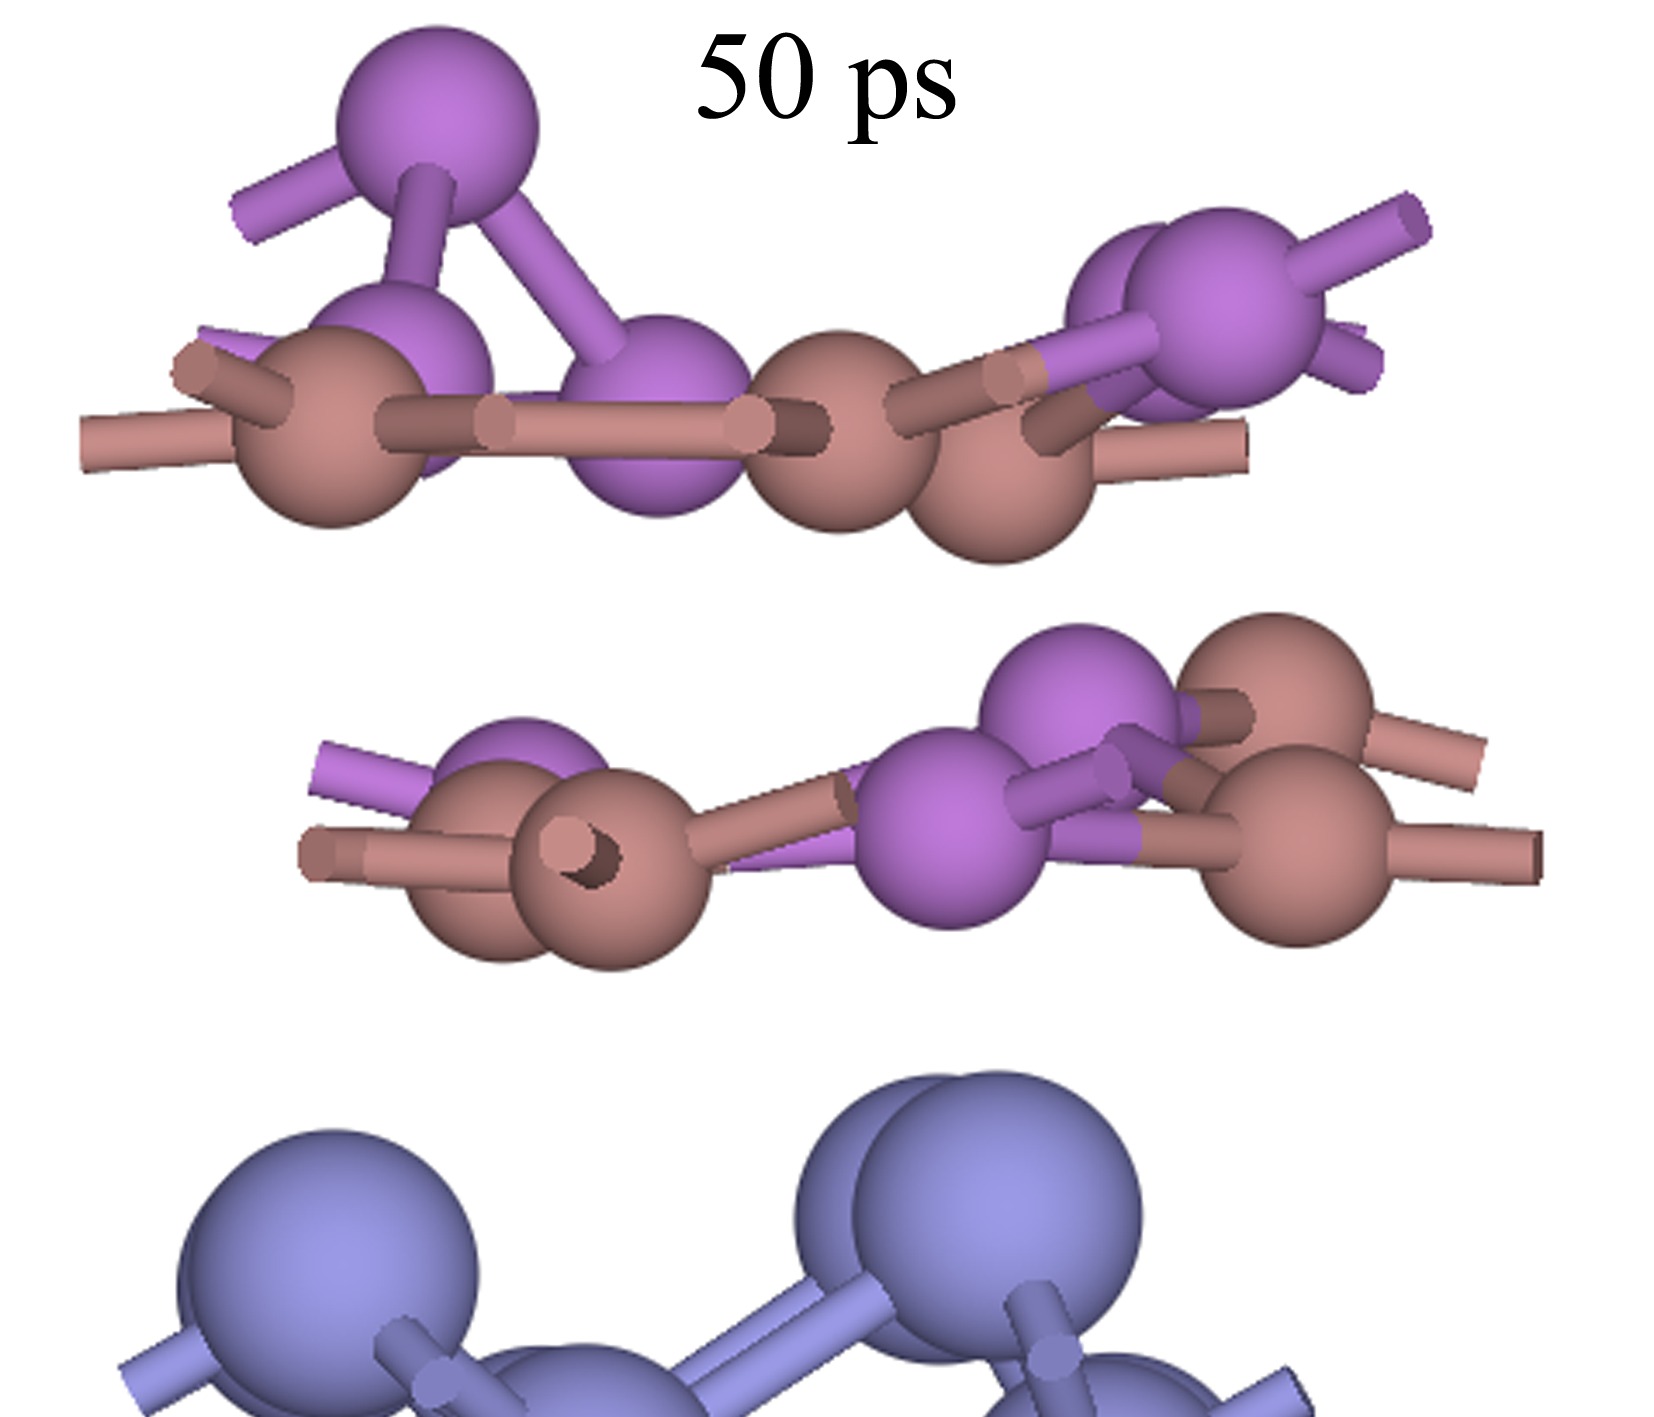
\includegraphics[width=0.35\textwidth]{pic/IS_structure_2Linsb_md50ps.png}
        \label{fig:IS_structure_2Linsb_md50ps}
    }
    \subfloat[]{
        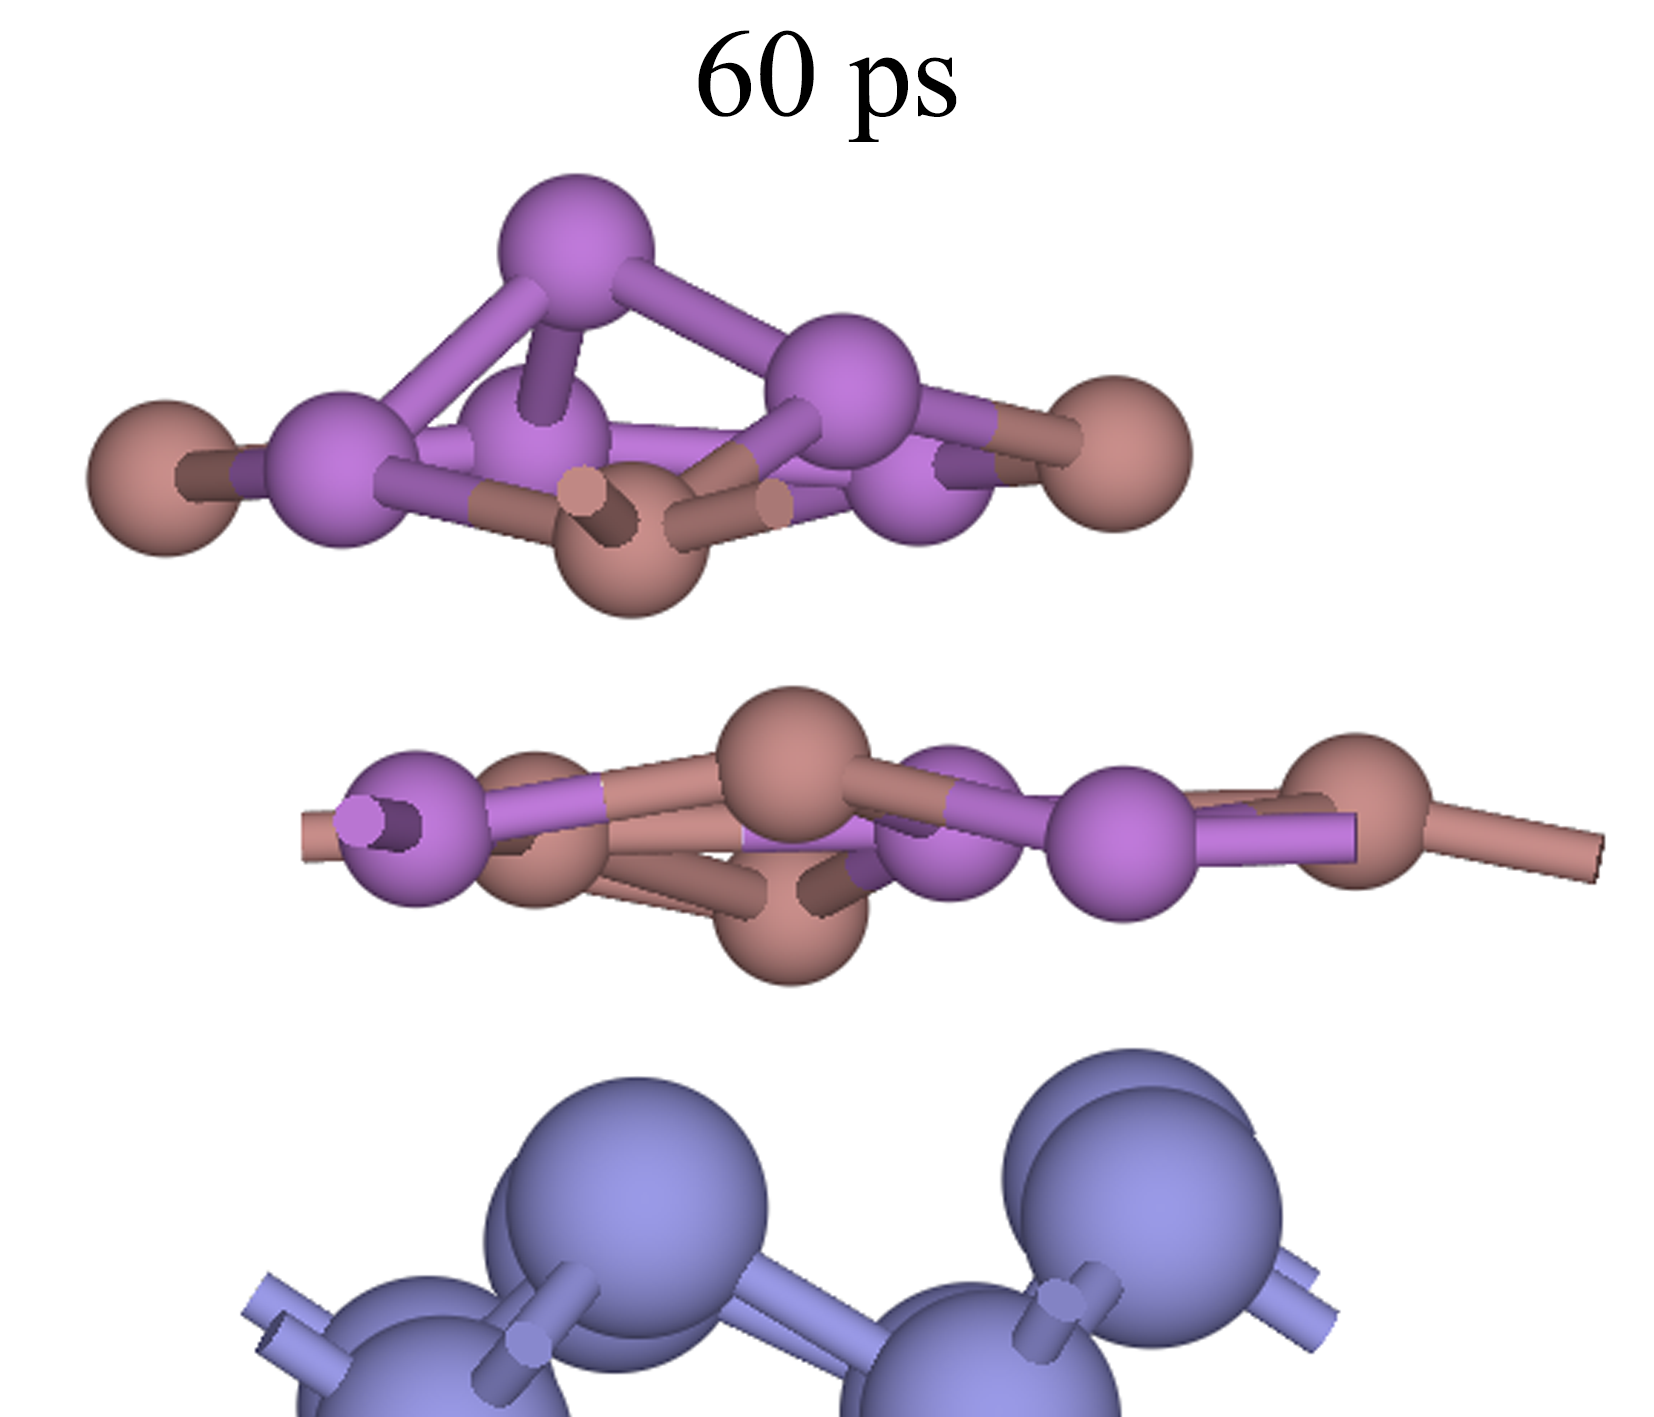
\includegraphics[width=0.35\textwidth]{pic/IS_structure_2Linsb_md60ps.png}
        \label{fig:IS_structure_2Linsb_md60ps}
    }\\[-1ex]
    \subfloat[]{
        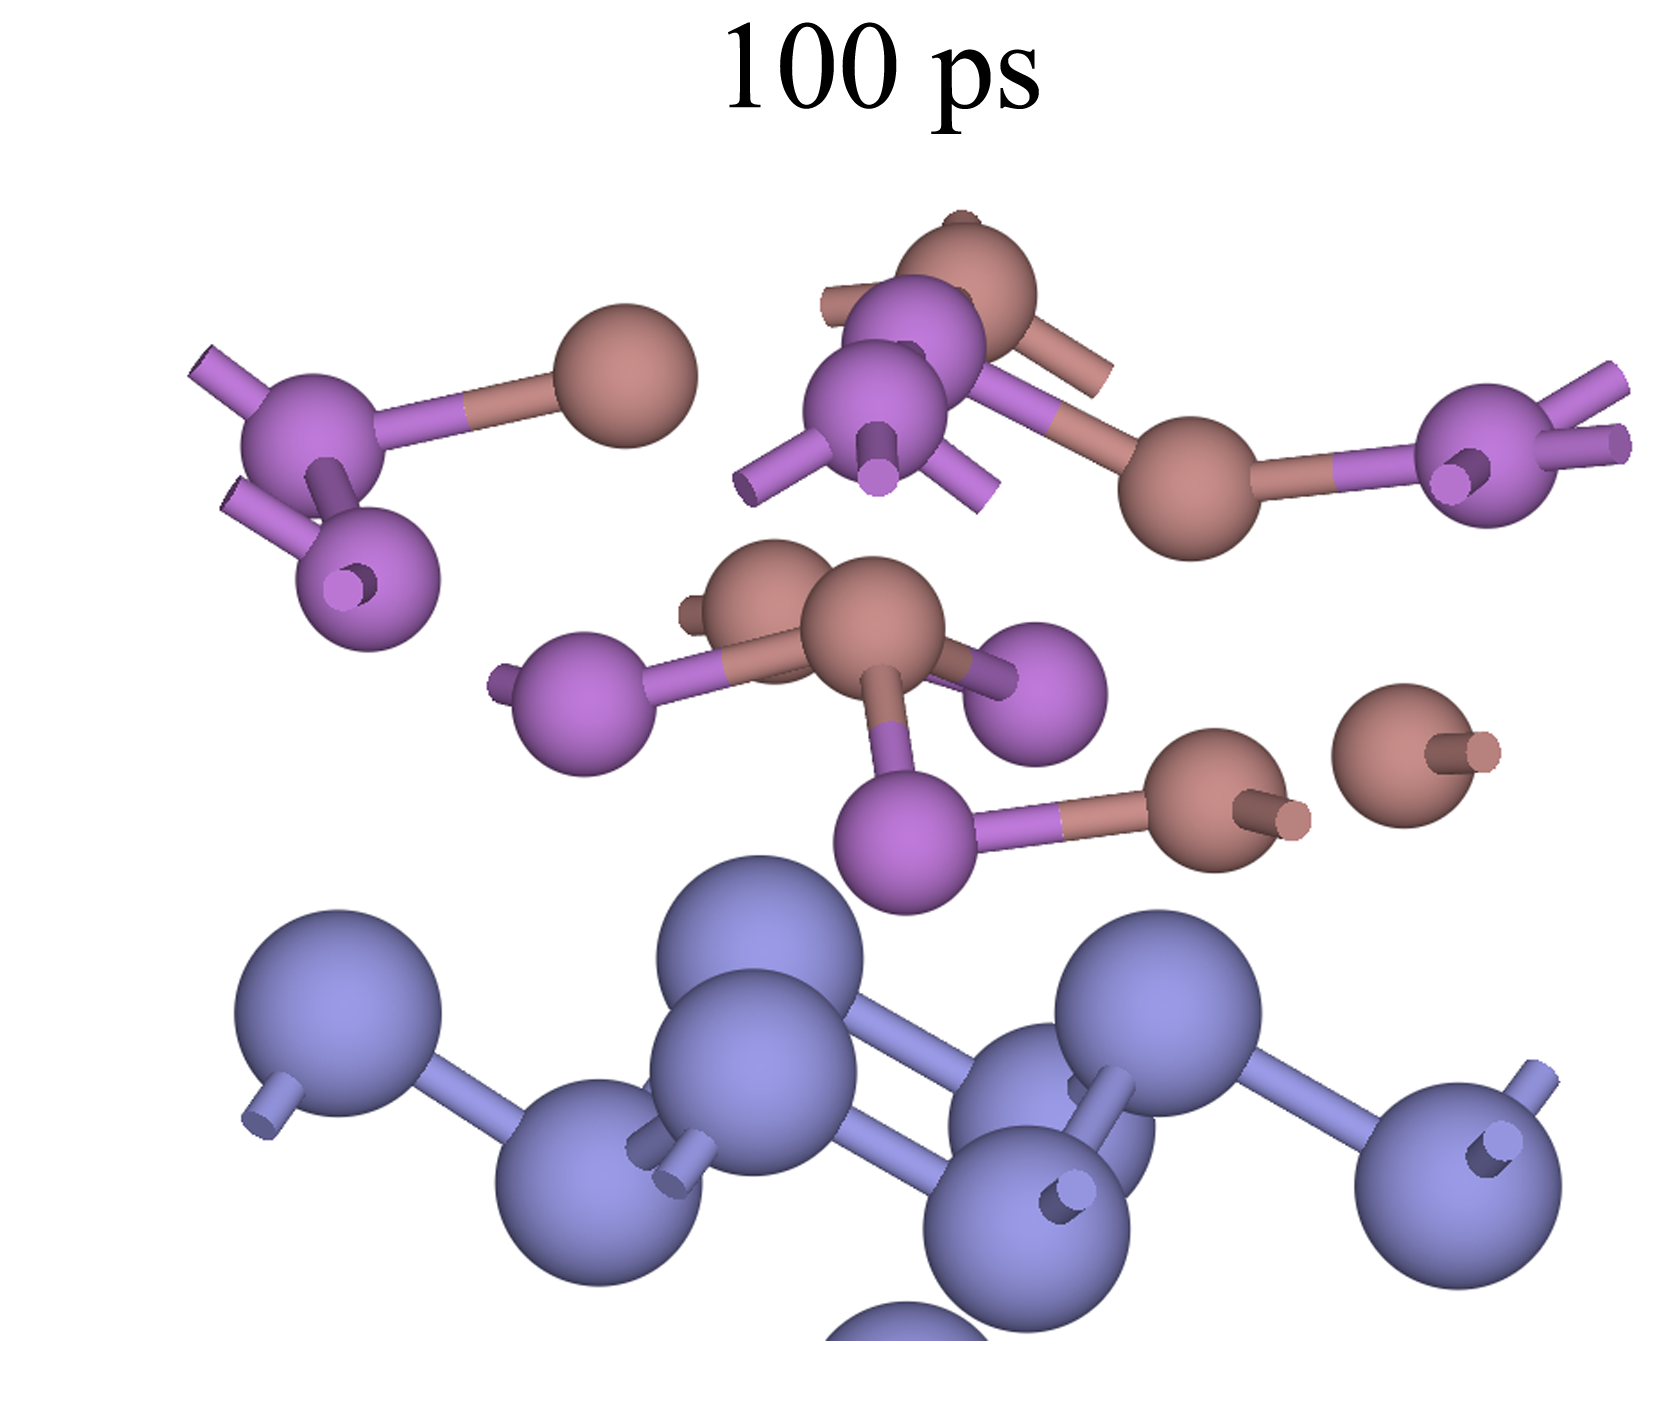
\includegraphics[width=0.35\textwidth]{pic/IS_structure_2Linsb_md100ps.png}
        \label{fig:IS_structure_2Linsb_md100ps}
    }
    \subfloat[]{
        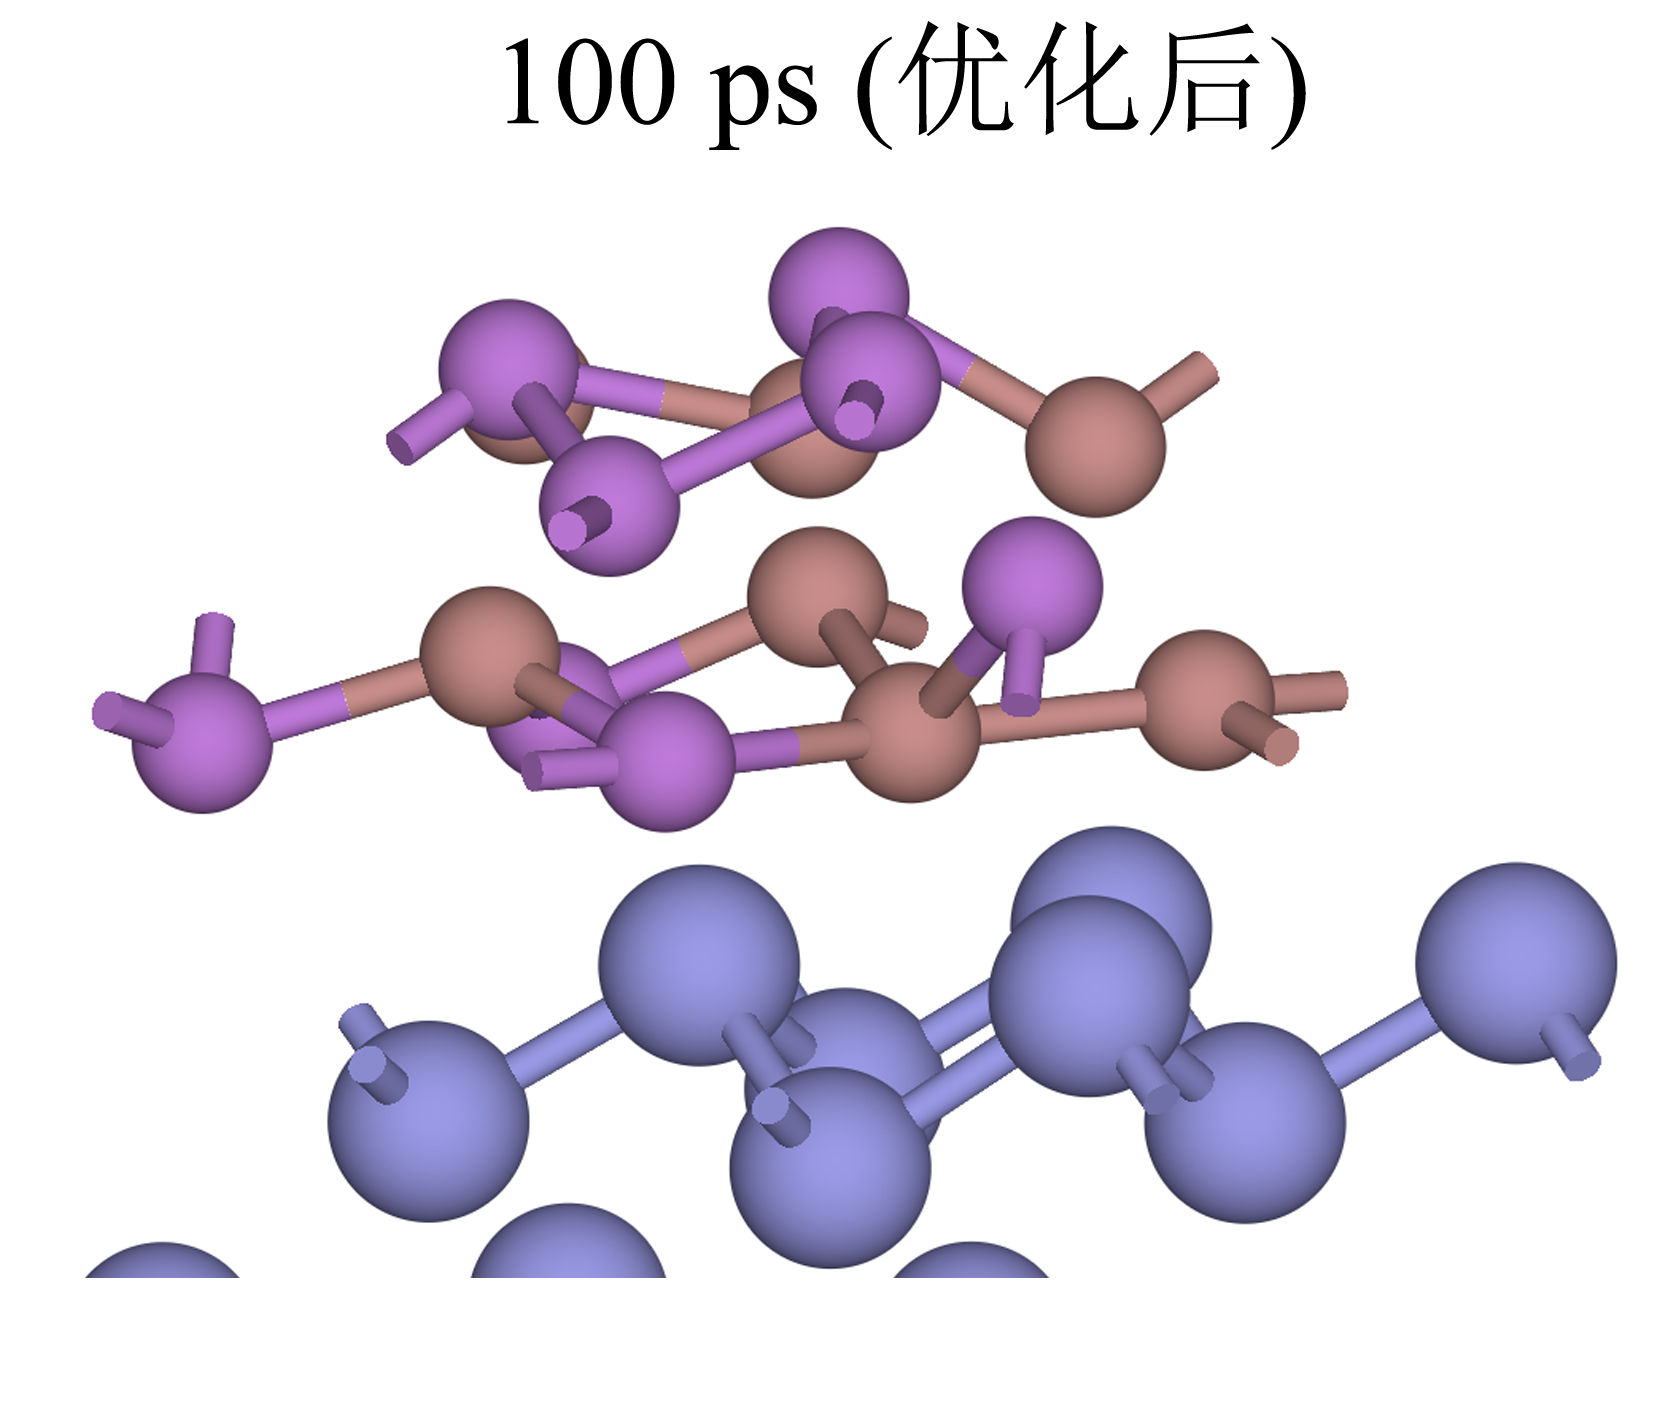
\includegraphics[width=0.35\textwidth]{pic/IS_structure_2Linsb_md100psopt.png}
        \label{fig:IS_structure_2Linsb_md100psopt}
    }
    \caption{\cemb{Bi(001)}衬底上双层\cemb{InSb}极性演化的分子动力学模拟结果。(a)分子动力学模拟50ps后的原子结构图;(b)分b动力学模拟60ps后的原子结构图;(c)分子动力学模拟100ps后的原子结构图;(d)100ps对应中间态的原子结构图。原子结构图中,\cemb{Bi}原子使用蓝色表示,\cemb{In}原子使用褐色表示,\cemb{Sb}原子使用紫色表示}
    \label{fig:IS_structure_2Linsb_md}
\end{figure}

由于计算能力和模拟时长的限制,本文未能在模拟的时限内发现\cemb{In}空位重构层下第一层\cemb{InSb}完全转变为\cemb{In}极化构型。本文对进行了分子动力学模拟\SI{100}{\pico\second}后的双层\cemb{InSb}模型进行了结构优化,以去除分子动力学模拟中的热扰动热扰动,获得在热动能的驱动下,双层\cemb{InSb}极性演化的中间态。如图\ref{fig:IS_structure_2Linsb_md100psopt}所示,在经过结构优化后,双层\cemb{InSb}极性演化的中间态具有两个\cemb{In}次表面四面体,显示出半\cemb{In}极化的结构。同时,形成能的计算显示这个双层\cemb{InSb}极性演化的中间态的形成能介于\cemb{In}极性的第一层和\InSbMLpolar{2}{2}的第一层之间。进一步印证了在热动能的驱使下,双层\cemb{InSb}会逐渐从原本以混合极性为主的非晶态慢慢极化至\cemb{In}极性。

为了揭示双层\cemb{InSb}的极化过程,本文首先对第二层\cemb{InSb}的生长过程进行探究。与在\cemb{Bi(001)}表面生长单层\cemb{InSb}类似,本文计算了\cemb{In}和\cemb{Sb}原子在单层\cemb{InSb}表面的吸附过程。考虑单层\cemb{InSb}以混合极性为主的非静态构型以及不同极性的形成能高低(图\ref{fig:IS_DFT_1LInSb_all}),本文选用\InSbMLpolar{2}{2}条形结构的单层\cemb{InSb}作为吸附表面。在图\ref{fig:IS_2Linsb_adatom}中,本文计算了单层\cemb{InSb}表面$\TfourSite$位和$\HthreeSite$位对于\cemb{In}和\cemb{Sb}原子的吸附能力。

\begin{figure}[!htb]
    \subfloat[]{
        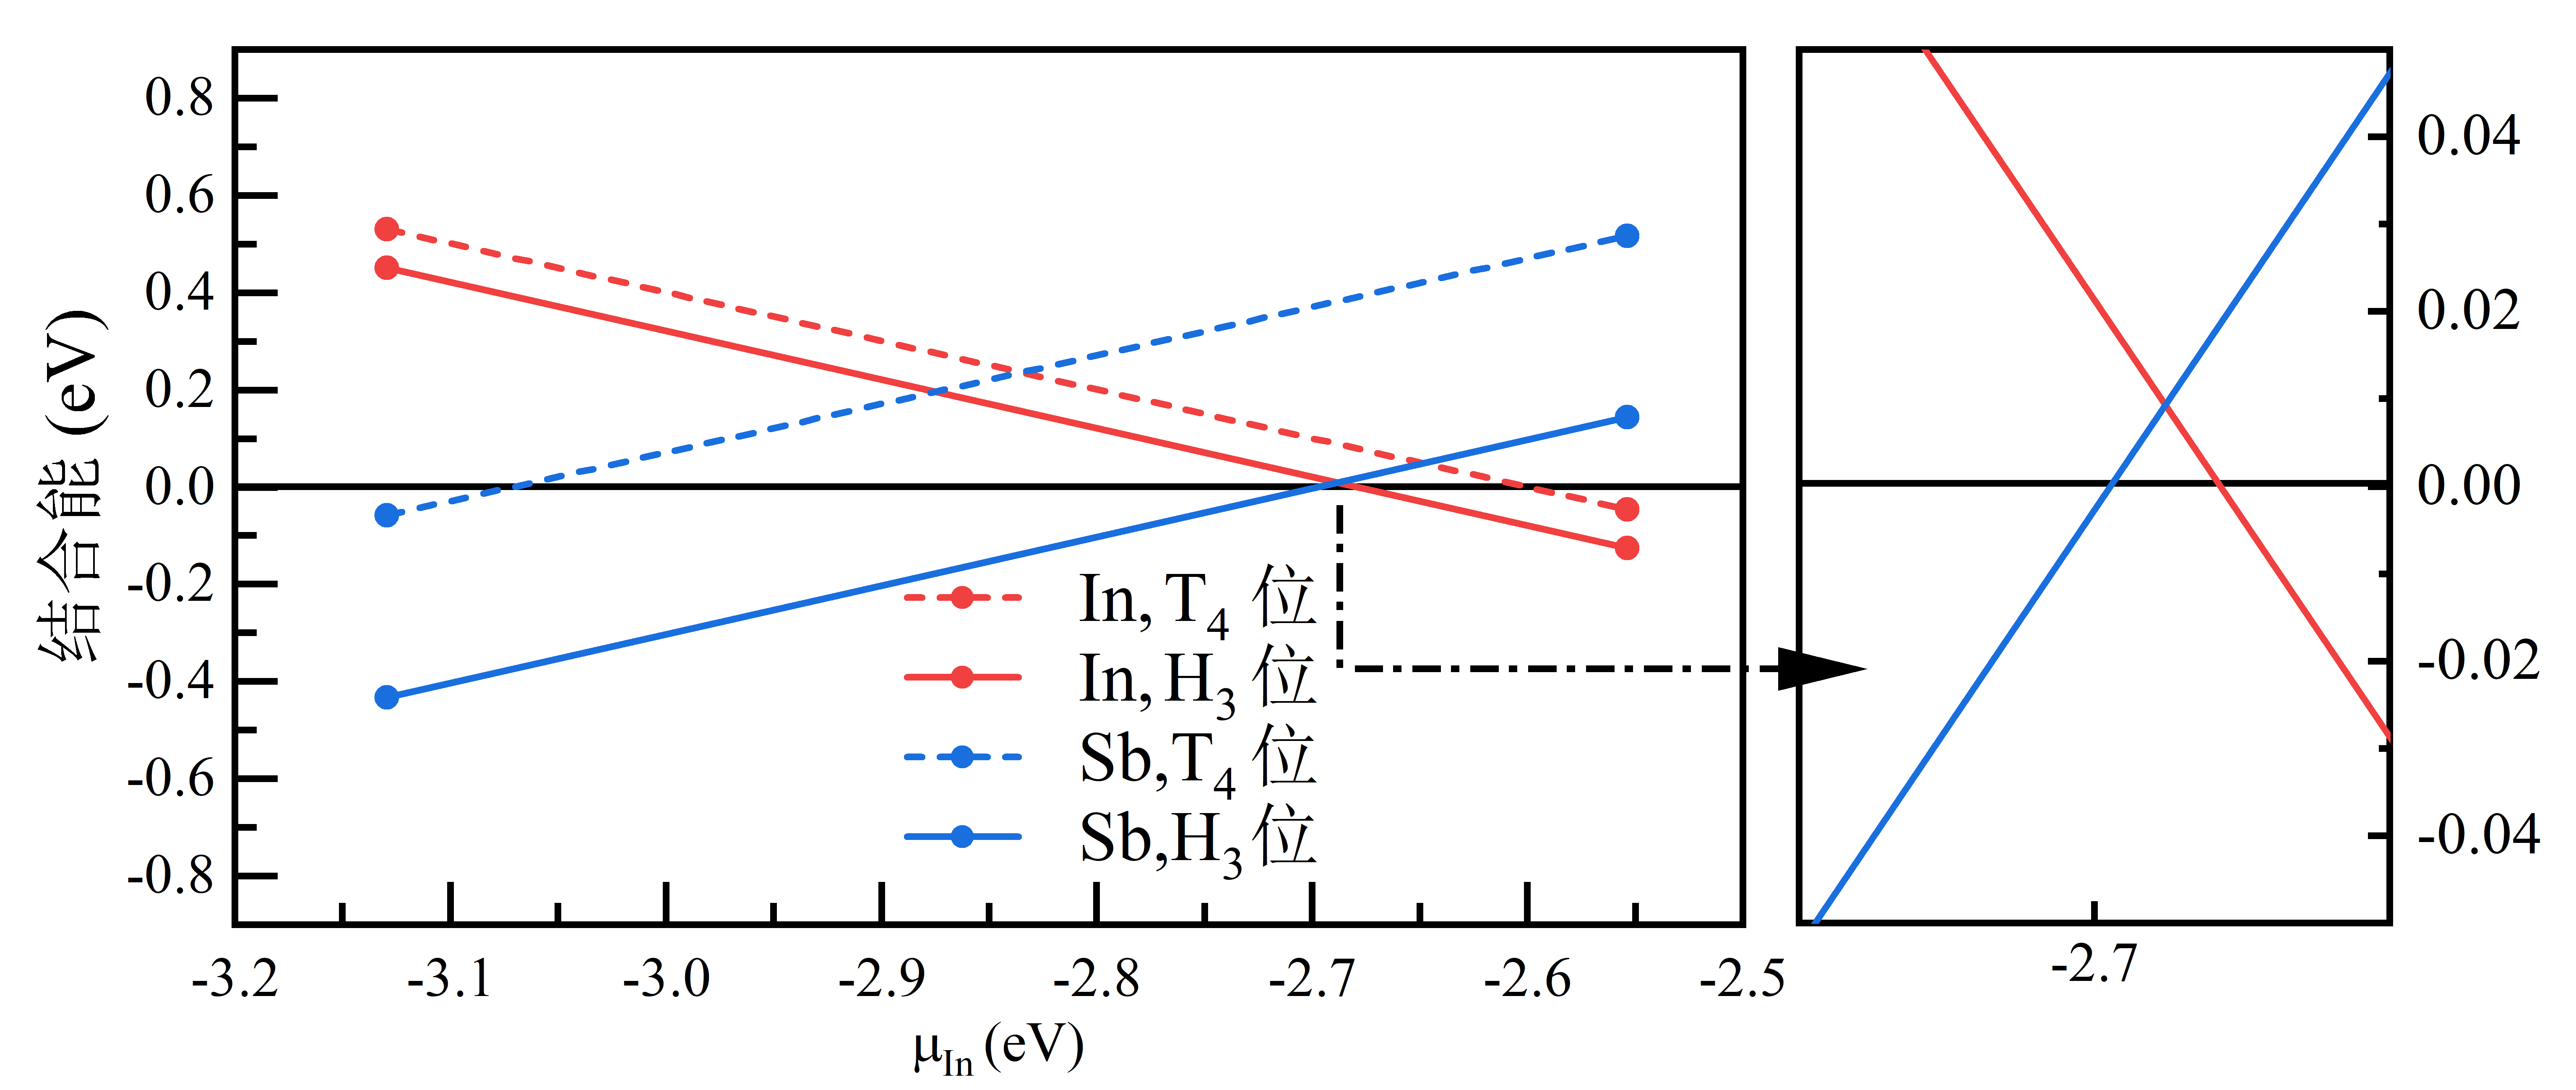
\includegraphics{pic/IS_DFT_2InSb_adatoms.png}
    }\\[-1ex]
    \subfloat[]{
        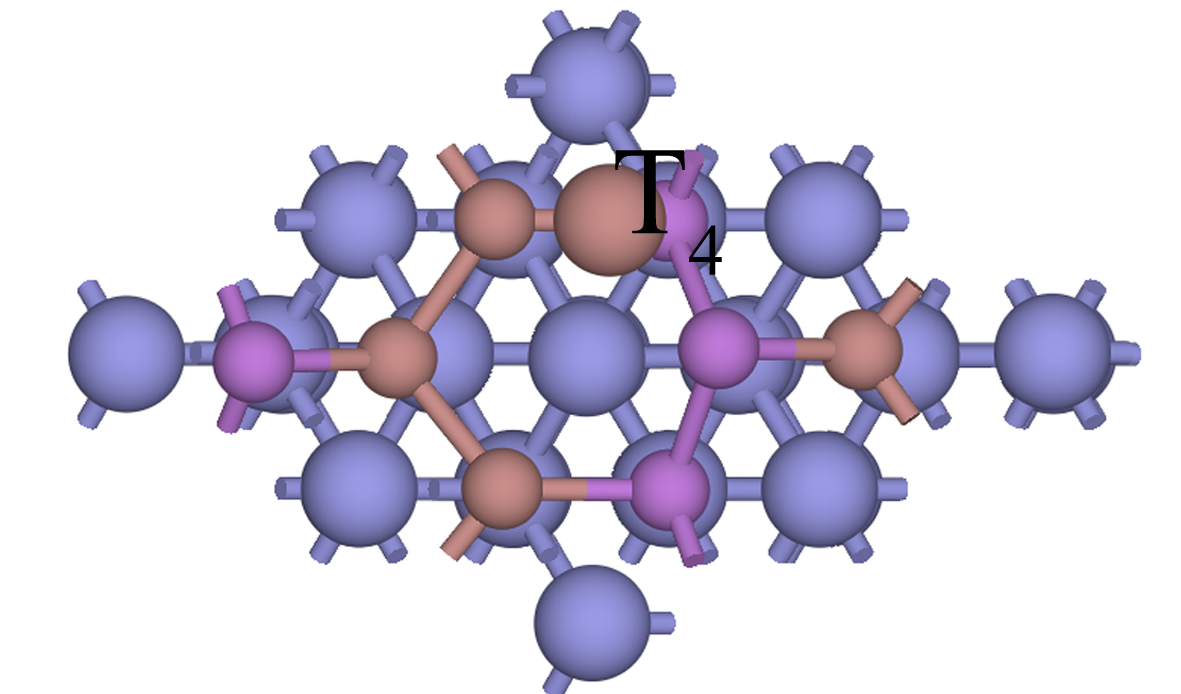
\includegraphics{pic/IS_structure_2Linsb_adatoms_InT4.png}
    }
    \subfloat[]{
        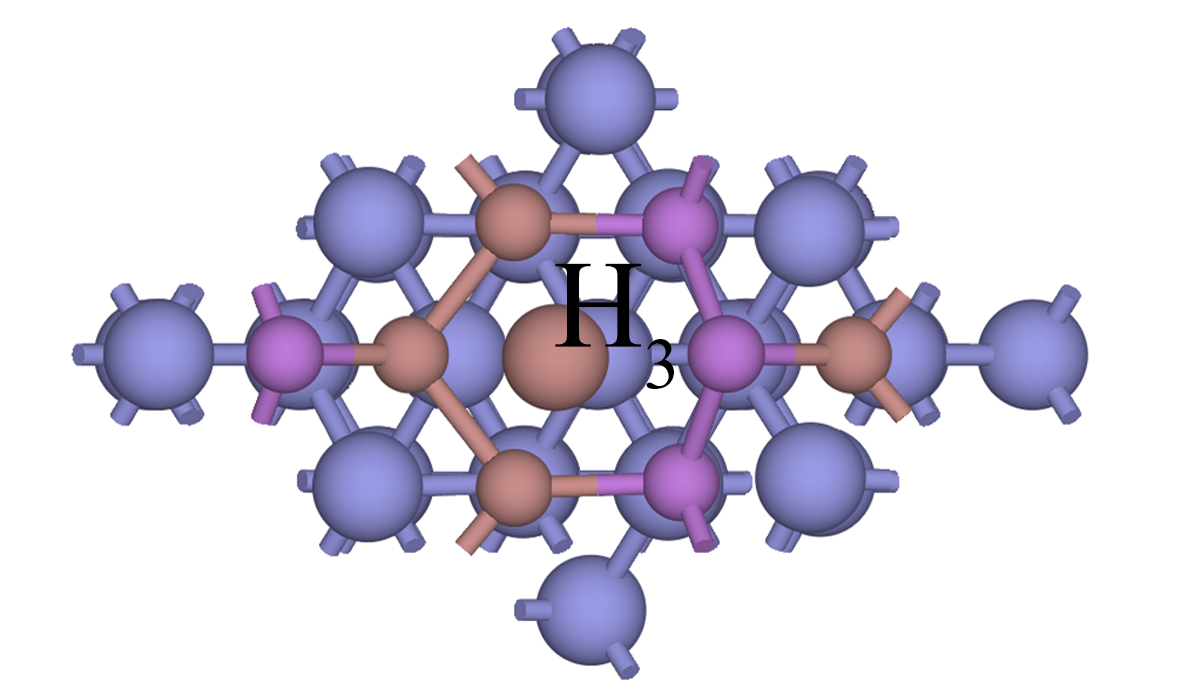
\includegraphics{pic/IS_structure_2Linsb_adatoms_InH3.png}
    }\\[-1ex]
    \subfloat[]{
        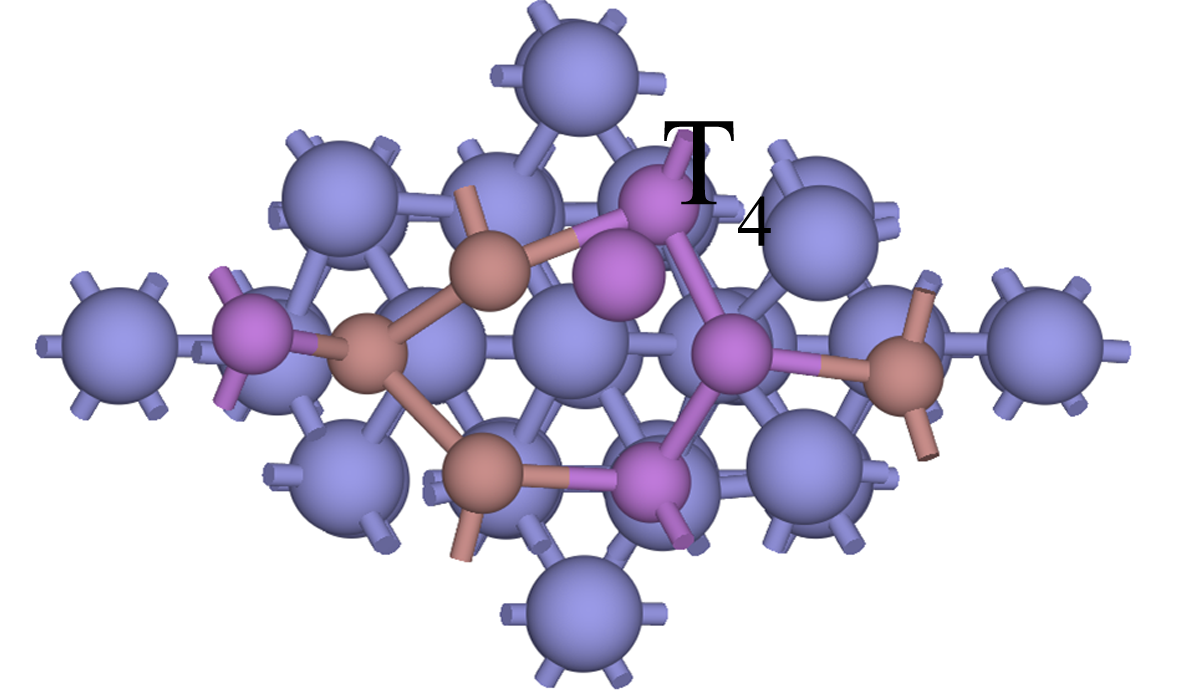
\includegraphics{pic/IS_structure_2Linsb_adatoms_SbT4.png}
    }
    \subfloat[]{
        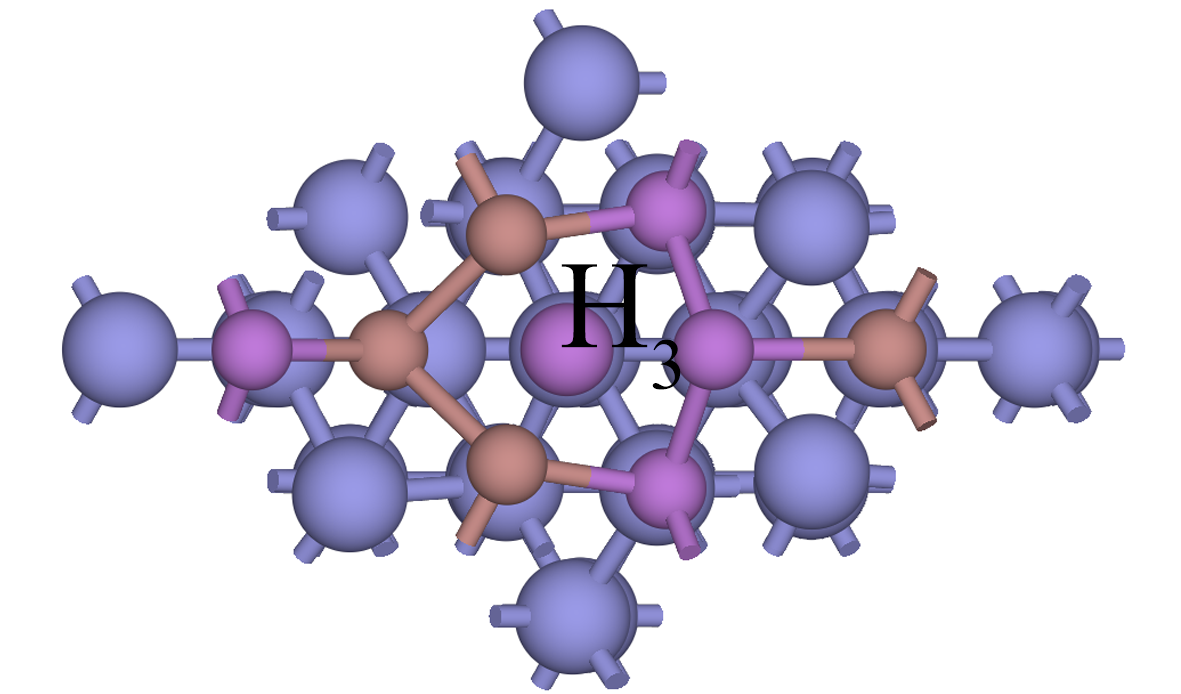
\includegraphics{pic/IS_structure_2Linsb_adatoms_SbH3.png}
    }
    \caption{\cemb{In}和\cemb{Sb}原子在\InSbMLpolar{2}{2}条形单层\cemb{InSb}表面吸附的结合能和吸附原子结构图。(a)吸附原子结合能;(b)\cemb{In}原子吸附在$\TfourSite$位;(c)\cemb{Sb}原子吸附在$\HthreeSite$位;(d)\cemb{In}原子吸附在$\TfourSite$位;(e)\cemb{Sb}原子吸附在$\HthreeSite$位。原子结构图中,\cemb{Bi}原子使用蓝色表示,\cemb{In}原子使用褐色表示,\cemb{Sb}原子使用紫色表示}
    \label{fig:IS_2Linsb_adatom}
\end{figure}

与在\cemb{Bi}表面吸附不同,单层\cemb{InSb}对于\cemb{In}原子的吸附能力弱于\cemb{Sb}原子。在各自的浓度比例极限中,\cemb{Sb}原子吸附在\cemb{InSb}表面具有比\cemb{In}原子更高的结合能。同时,\cemb{Sb}原子与单层\cemb{InSb}更强的相互作用使得\cemb{Sb}原子吸附的为放热反应的$\muVar{In}{}$范围宽于\cemb{In}原子。对于\cemb{Sb}原子而言,其可以在生长环境中\cemb{In}原子浓度略高的情况下在单层\cemb{InSb}的表面吸附($\muVar{In}{}\leqslant \SI{-2.70}{\electronvolt}$)。而\cemb{In}原子只能在$\muVar{In}{} \geqslant \SI{-2.68}{\electronvolt}$的生长环境下才倾向于在单层的\cemb{InSb}表面吸附。在\InSbMLpolar{2}{2}条形结构的\cemb{InSb}的表面,没有能够同时吸附\cemb{In}原子和\cemb{Sb}原子的$\muVar{In}{}$窗口。因此,在第二层\cemb{InSb}成核生长的早期,由于生长环境中原子比例和化学活性的不同,在\cemb{In}和\cemb{Sb}之间只有一种原子能够直接在单层\cemb{InSb}表面吸附。可以通过调节生长环境中的浓度比例调控在单层\cemb{InSb}的优先吸附原子类型。

随着生长的进行,原本难以在单层\cemb{InSb}表面吸附的原子可能和已吸附的原子成键,形成团簇。团簇的生长形态和化学组成同样可能受到生长环境中$\muVar{In}{}$变化的影响。考虑第二层为到\cemb{Sb}三聚体重构时,从双层\cemb{InSb}的形成能谱(图\ref{fig:IS_DFT_2LInSb_SbTonAll})可以看出,第一层混合极性的\cemb{InSb}的晶体化转变开始于作为第二层的\cemb{Sb}团簇重构层将第一层引导至理想极性的构型(\cemb{In}极性或者\cemb{Sb}极性)。

在生长过程的团簇阶段,需要验证\cemb{Sb}三聚体是否是生长过程中最为可能的团簇形态。因此,本文进一步考察了团簇生长阶段不同形貌的三聚体在\cemb{InSb}自极化过程中的形貌以及作为第二层的\cemb{InSb}团簇在不同$\muVar{In}{}$环境下的演化规律(图\ref{fig:IS_structure_InxSb3-x})。

\begin{figure}[!htb]
    \subfloat[]{
        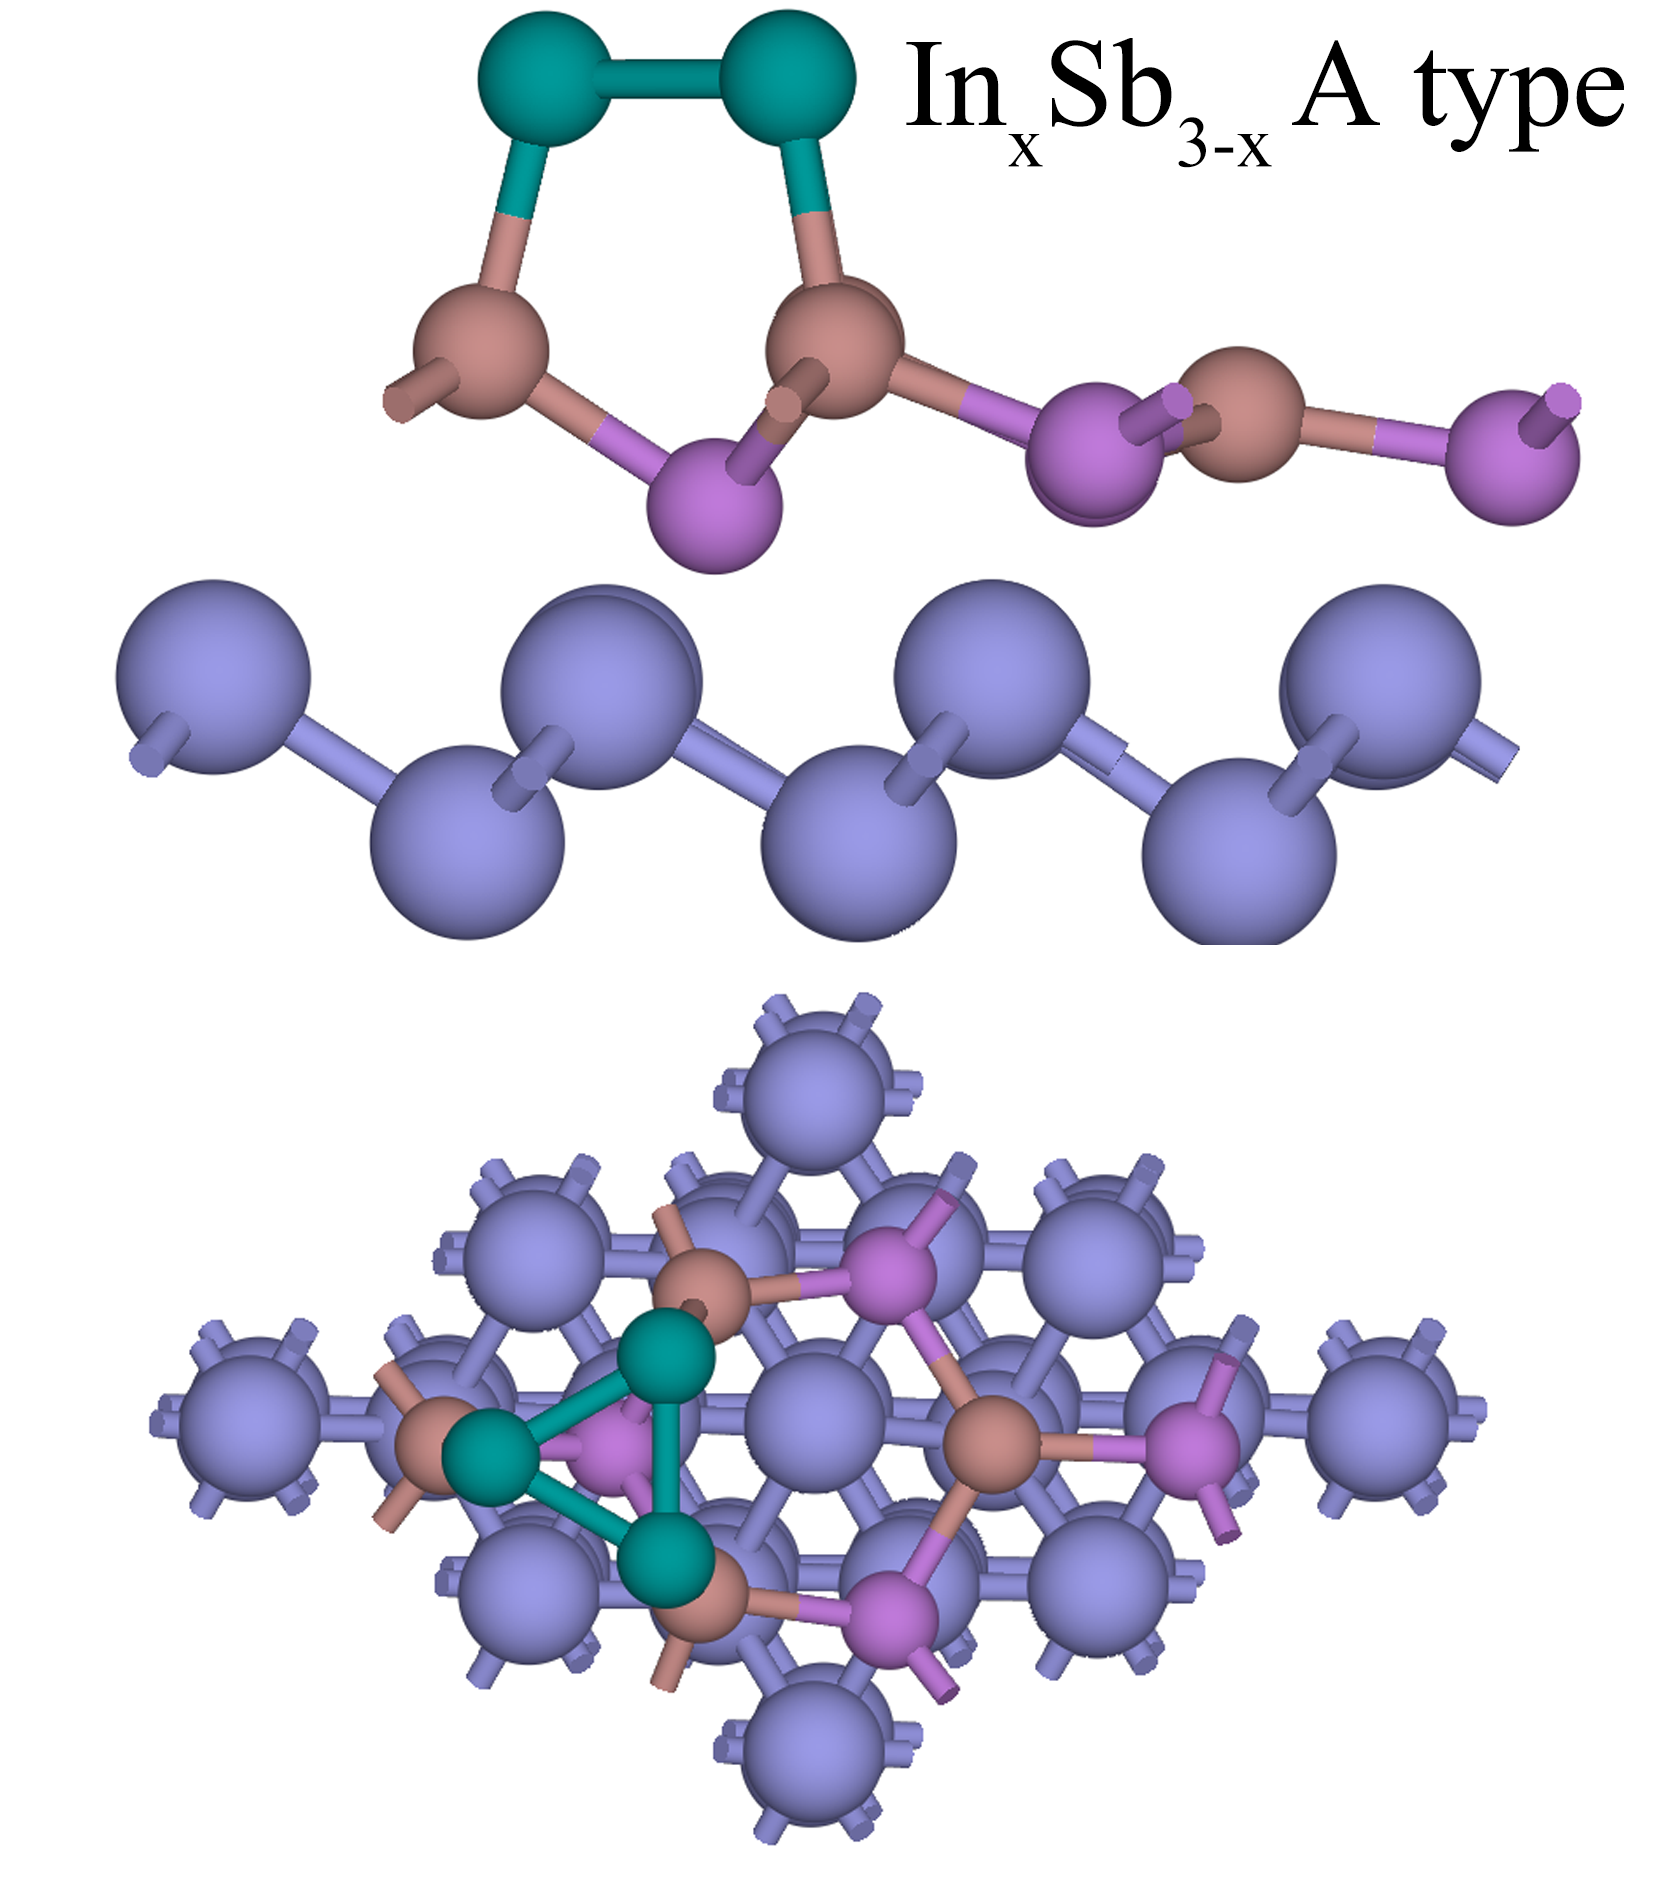
\includegraphics[scale=0.7]{pic/IS_structure_InxSb3-x_A.png}
    }
    \subfloat[]{
        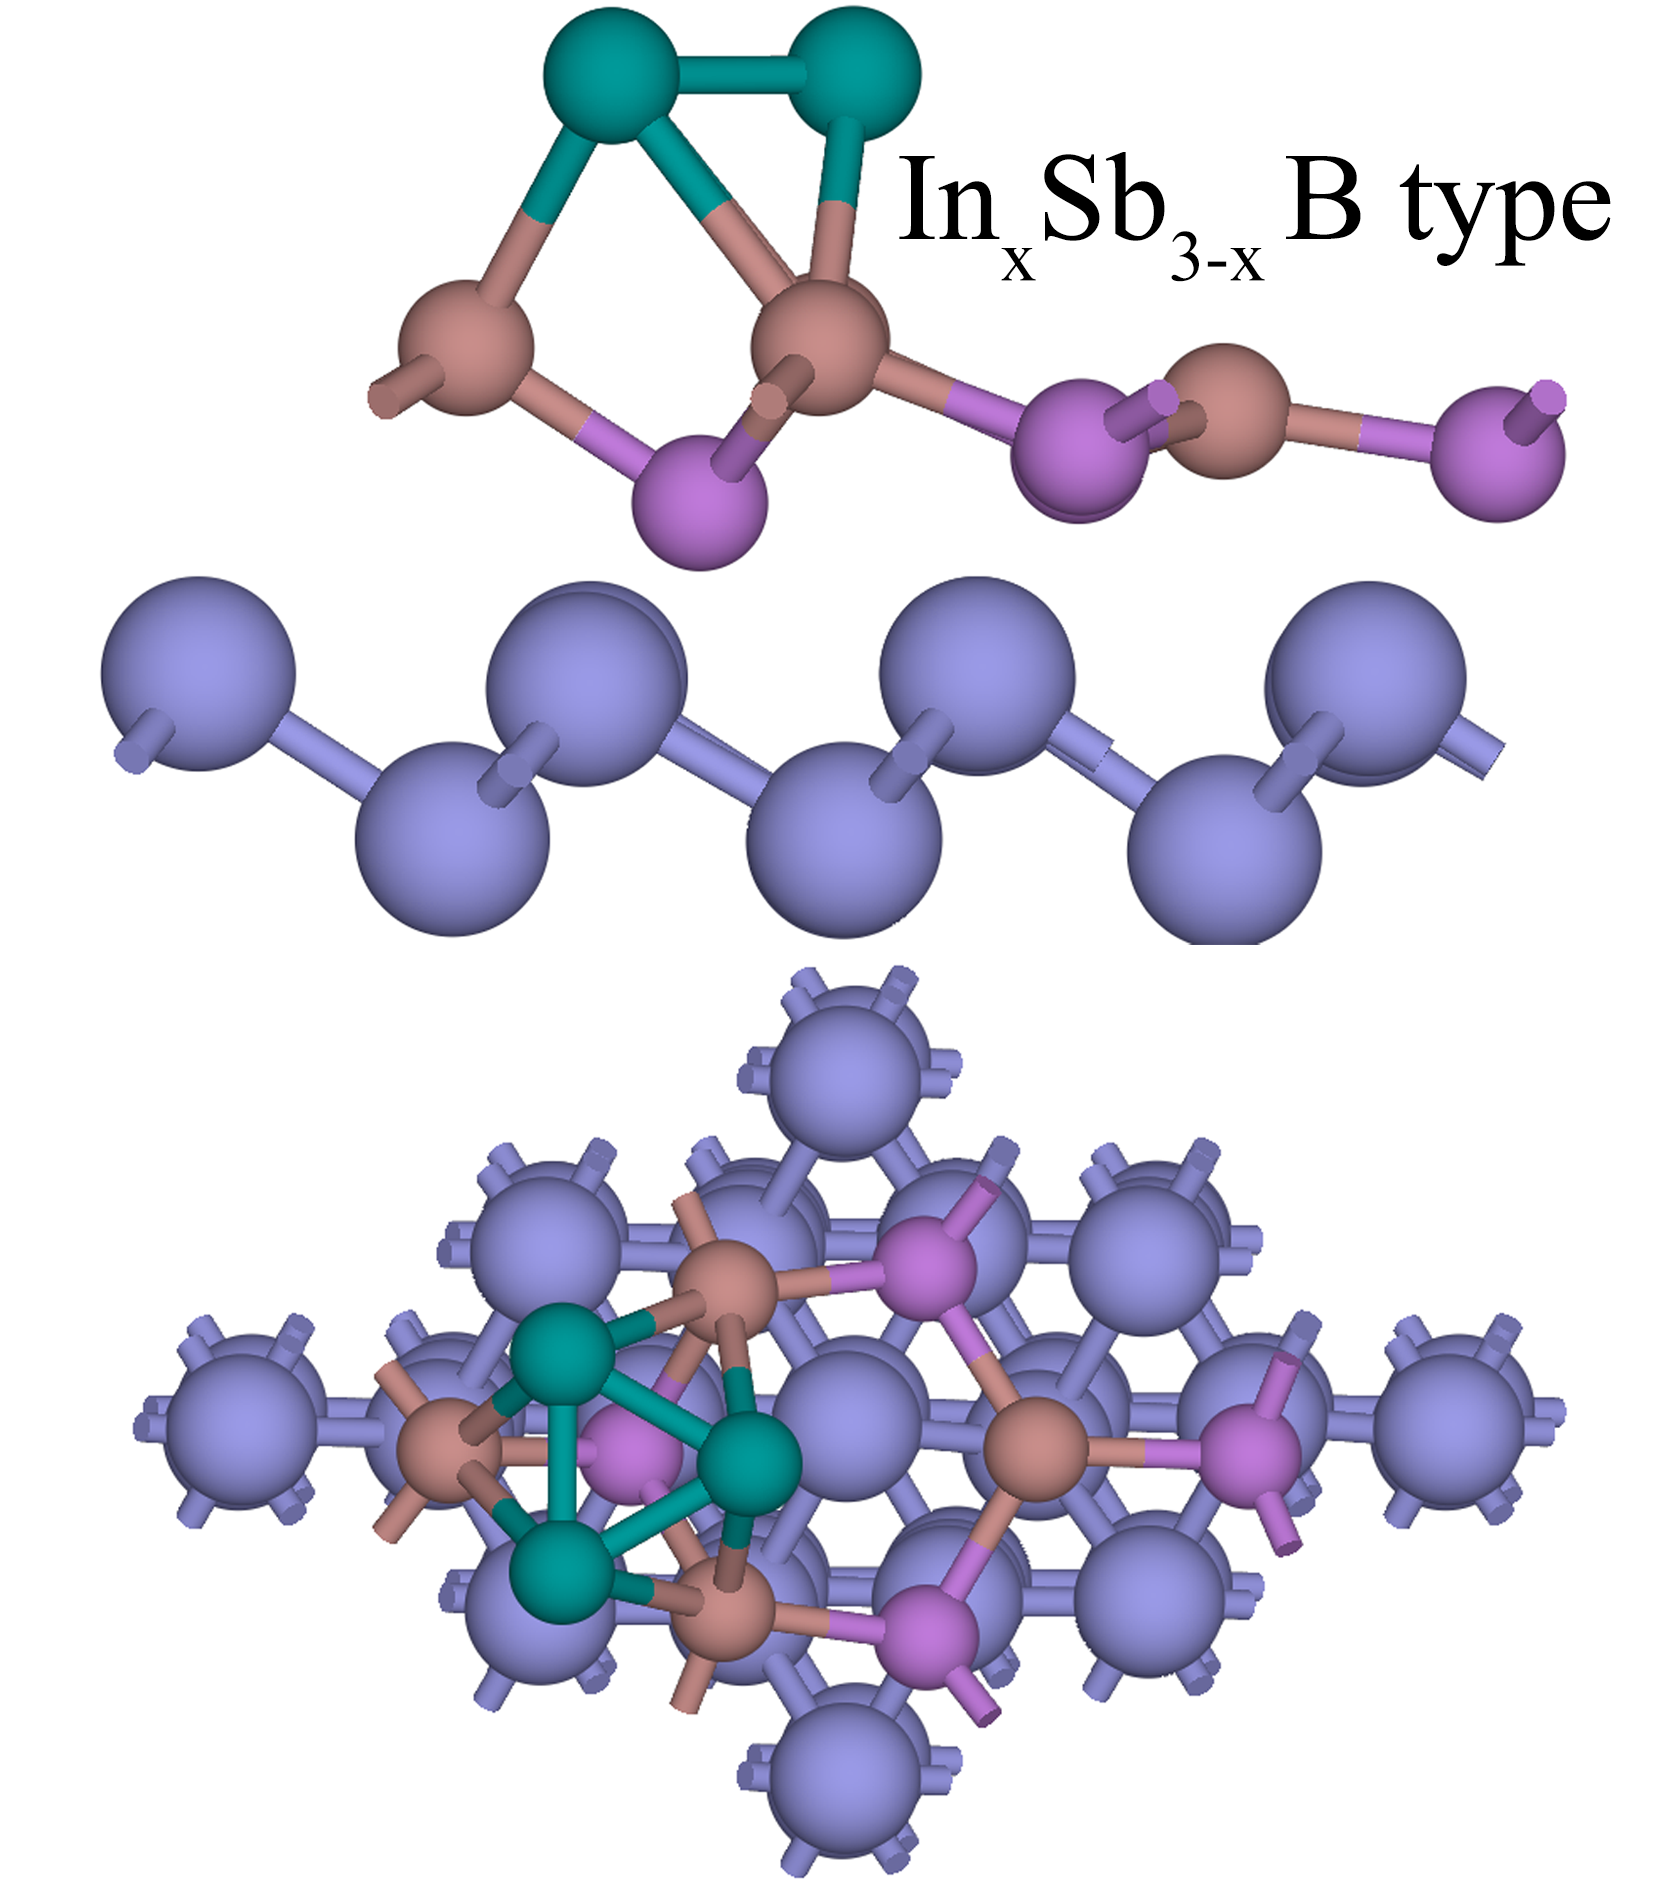
\includegraphics[scale=0.7]{pic/IS_structure_InxSb3-x_B.png}
    }
    \caption{单层\cemb{InSb}表面生长团簇(\cemb{In_xSb_{3-x}})的构型。(a)A类\cemb{In_xSb_{3-x}}团簇的原子构型;(b)B类\cemb{In_xSb_{3-x}}团簇的原子构型。原子结构图中,\cemb{Bi}原子使用蓝色表示,团簇原子(\cemb{In}、\cemb{Sb})用绿色表示}
    \label{fig:IS_structure_InxSb3-x}
\end{figure} 

通过先前的计算,已经得知作为第二层的\cemb{Sb}三聚体重构可以将原本极性混乱的第一层\cemb{InSb}引导至\cemb{In}极性或者\cemb{Sb}极性。而\cemb{In}极性的第一层构型是以\cemb{Sb}三聚体重构为第二层的双层石墨烯的全局能量最低态。因此,本文将第一层构型的关注点限定在\cemb{In}极性,考察不同元素比例的\cemb{In_xSb_{3-x}}三聚体的生长机理。将\cemb{In}极性\cemb{InSb}上生长的\cemb{In_xSb_{3-x}}三聚体分为两类,A类的构型和先前所计算的\cemb{Sb}三聚体类似,三聚体内部的原子处于$\TfourSite$位三角形的顶点位。B类构型由A类构型在平面内旋转\SI{60}{\degree}得到,其三聚体内部的原子处于$\TfourSite$位三角形的边位。

在图\ref{fig:IS_DFT_2InSb_InxSbxT_All}中,本文计算了在\cemb{In}极性的\cemb{InSb}表面生长不同化学计量比的$\cemb{In_xSb_{3-x}}$团簇的形成能情况。整体来看,随着\cemb{Sb}原子化学计量比的上升,\cemb{In_xSb_{3-x}}团簇的形成能逐渐下降。在所有考虑的团簇中, A类\cemb{In0Sb3}团簇(\cemb{Sb}三聚体重构)的形成能在在大部分的$\muVar{In}{}$条件下取到最低值。这与\cemb{Sb}三聚体重构作为生长实验中自然形成的\cemb{Sb}极性的表面重构现象一致\citing{RN896-1998}。而包含\cemb{In}元素的团簇仅在生长环境中\cemb{In}原子浓度较高,$\muVar{In}{}$的取值接近纯\cemb{In}极限时才有能量上的优势。

\begin{figure}[!htb]
    \subfloat[]{
        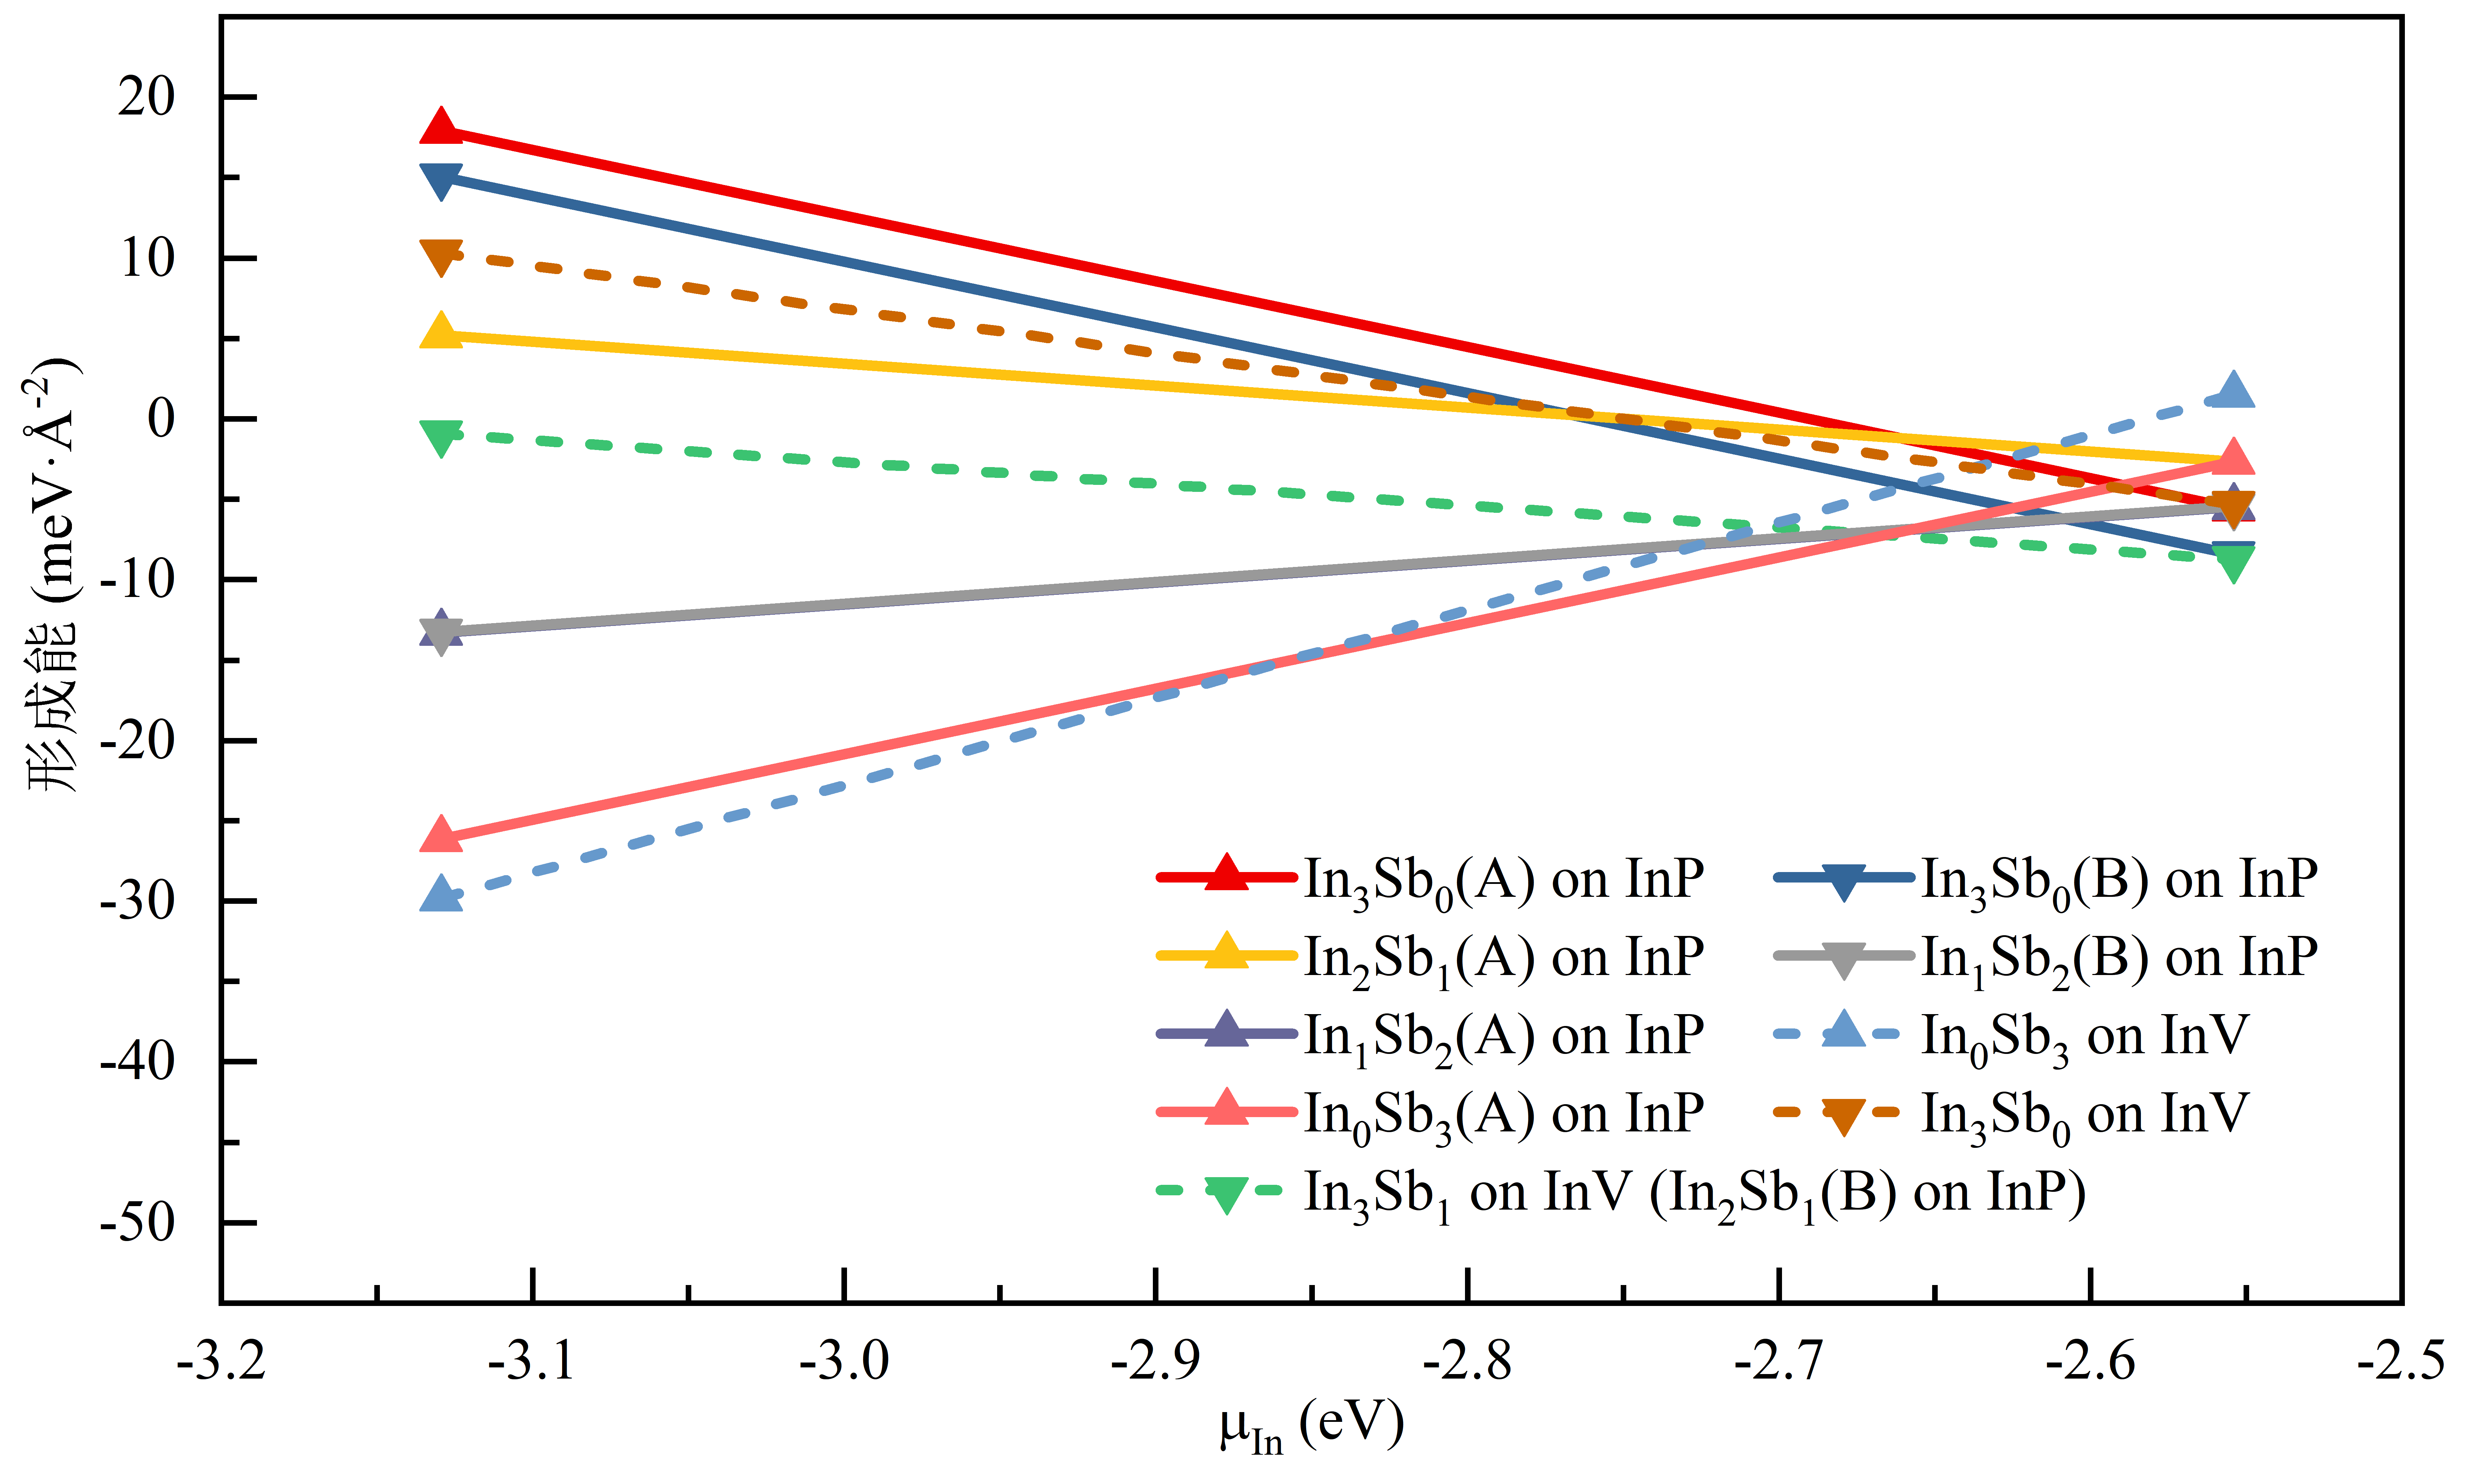
\includegraphics[width=0.9\textwidth]{pic/IS_DFT_2InSb_InxSbxT_All.png}
    }\\[-1ex]
    \subfloat[]{
        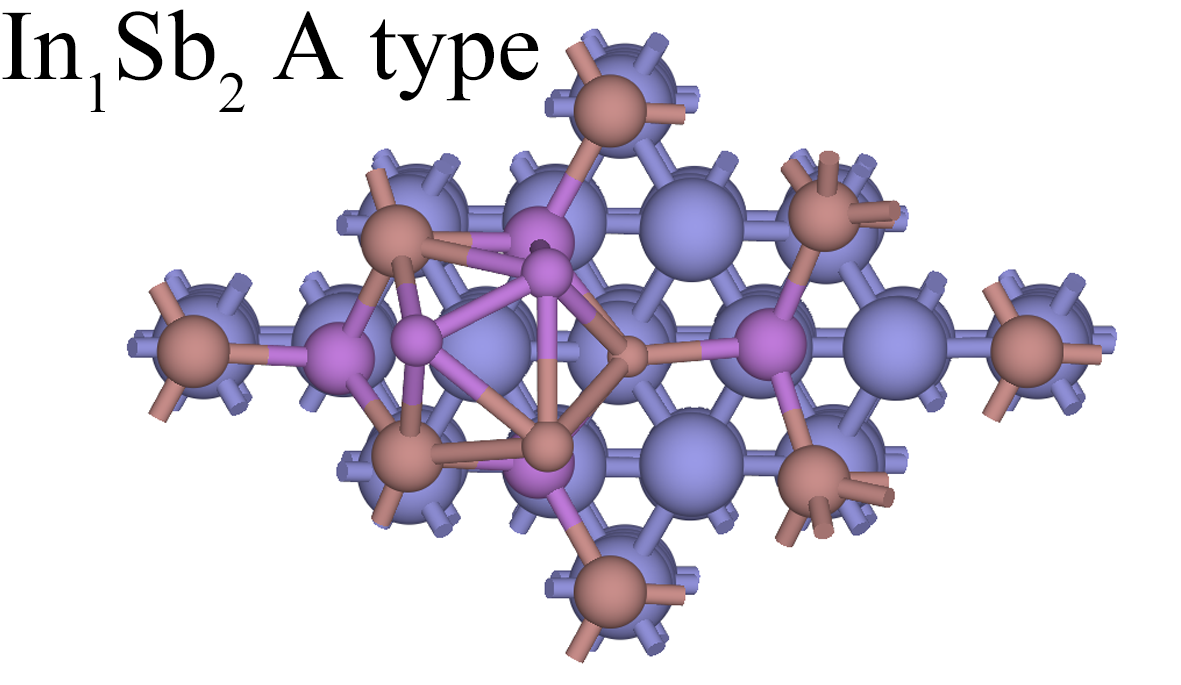
\includegraphics[width=0.3\textwidth]{pic/IS_structure_In1Sb2_A.png}
    }
    \subfloat[]{
        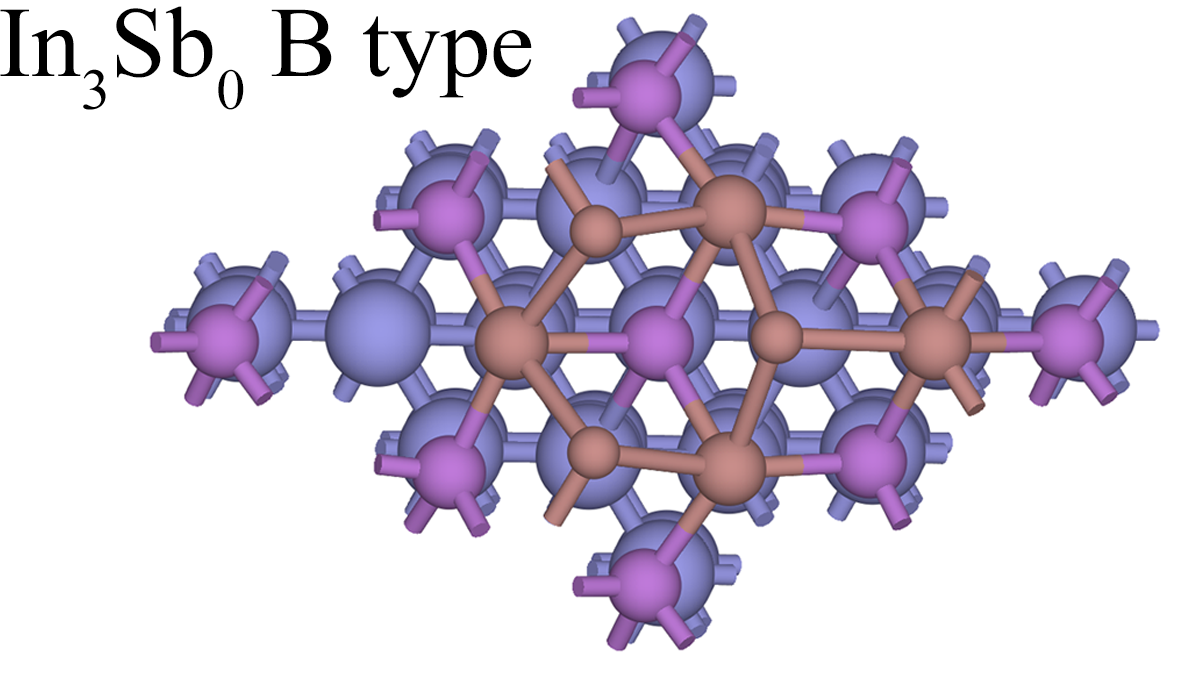
\includegraphics[width=0.3\textwidth]{pic/IS_structure_In3Sb0_B.png}
    }
    \subfloat[]{
        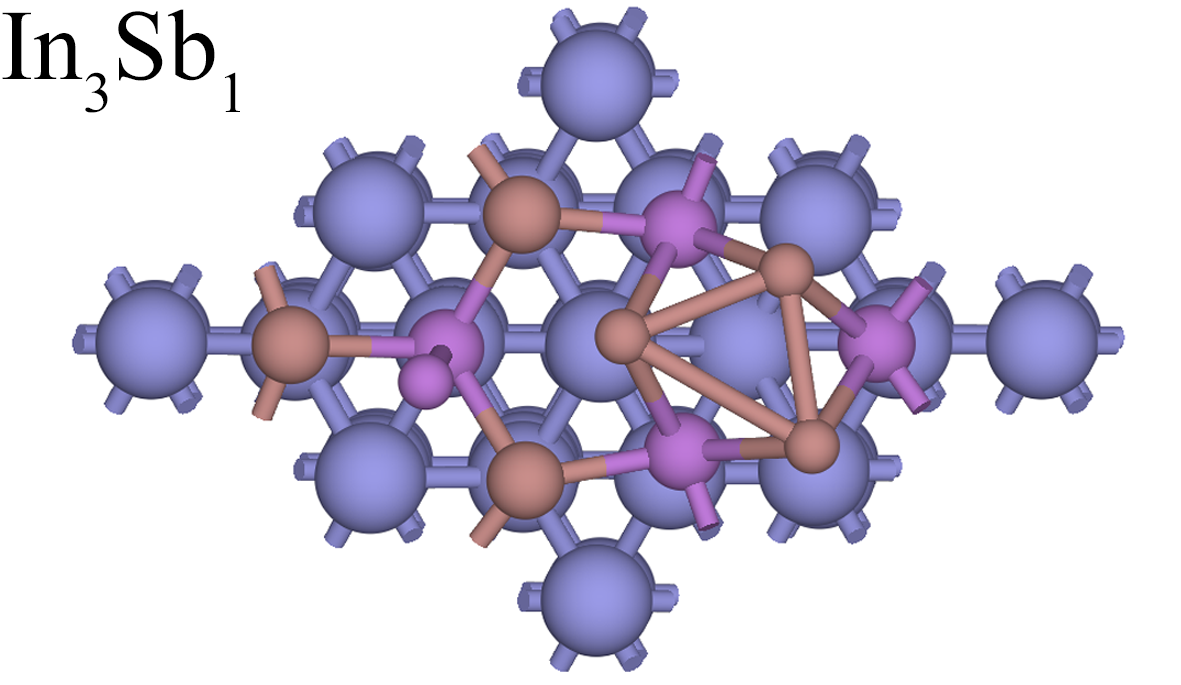
\includegraphics[width=0.3\textwidth]{pic/IS_structure_In3Sb1.png}
    }
    \caption{单层\cemb{InSb}表面\cemb{In_xSb_{3-x}}团簇的形成能及代表性团簇结构原子构型。(a)不同化学计量比\cemb{In_xSb_{3-x}}团簇的形成能分布;(b)A类\cemb{In1Sb2}的原子构型;(c)B类\cemb{In3Sb0}的原子构型。原子结构图中,\cemb{Bi}原子使用蓝色表示,\cemb{In}原子使用褐色表示,\cemb{Sb}原子使用紫色表示}
    \label{fig:IS_DFT_2InSb_InxSbxT_All}
\end{figure}

从原子结构的角度看,\cemb{Sb}原子在\cemb{InSb}表面形成的重构倾向于保持A类团簇的构型,而\cemb{In}原子组成的重构则倾向于形成B类团簇的结构。在\cemb{InSb}混合团簇的原子结构中,\cemb{In}的加入更倾向于单独吸附在$\TfourSite$位点,破坏了\cemb{Sb}三聚体在\cemb{InSb}表面的等边三角形构型。对于只含有\cemb{In}原子的\cemb{In3Sb0}团簇,结构优化的结果显示第二层的\cemb{In}原子之间仅存在非常弱的相互作用。这个较弱的相互作用只将原本各自独立吸附在$\TfourSite$位和$\HthreeSite$位的\cemb{In}原子向团簇的中心偏移了很小的位移。综合以上的计算结果,可以认为在生长第二层\cemb{InSb}以及双层\cemb{InSb}的自极化过程中,团簇阶段主要以\cemb{Sb}三聚体的形式存在。而在团簇阶段中\cemb{InSb}第一层表面的\cemb{In}原子则主要以较为分散的吸附原子的形式存在。

\begin{figure}[htb]
    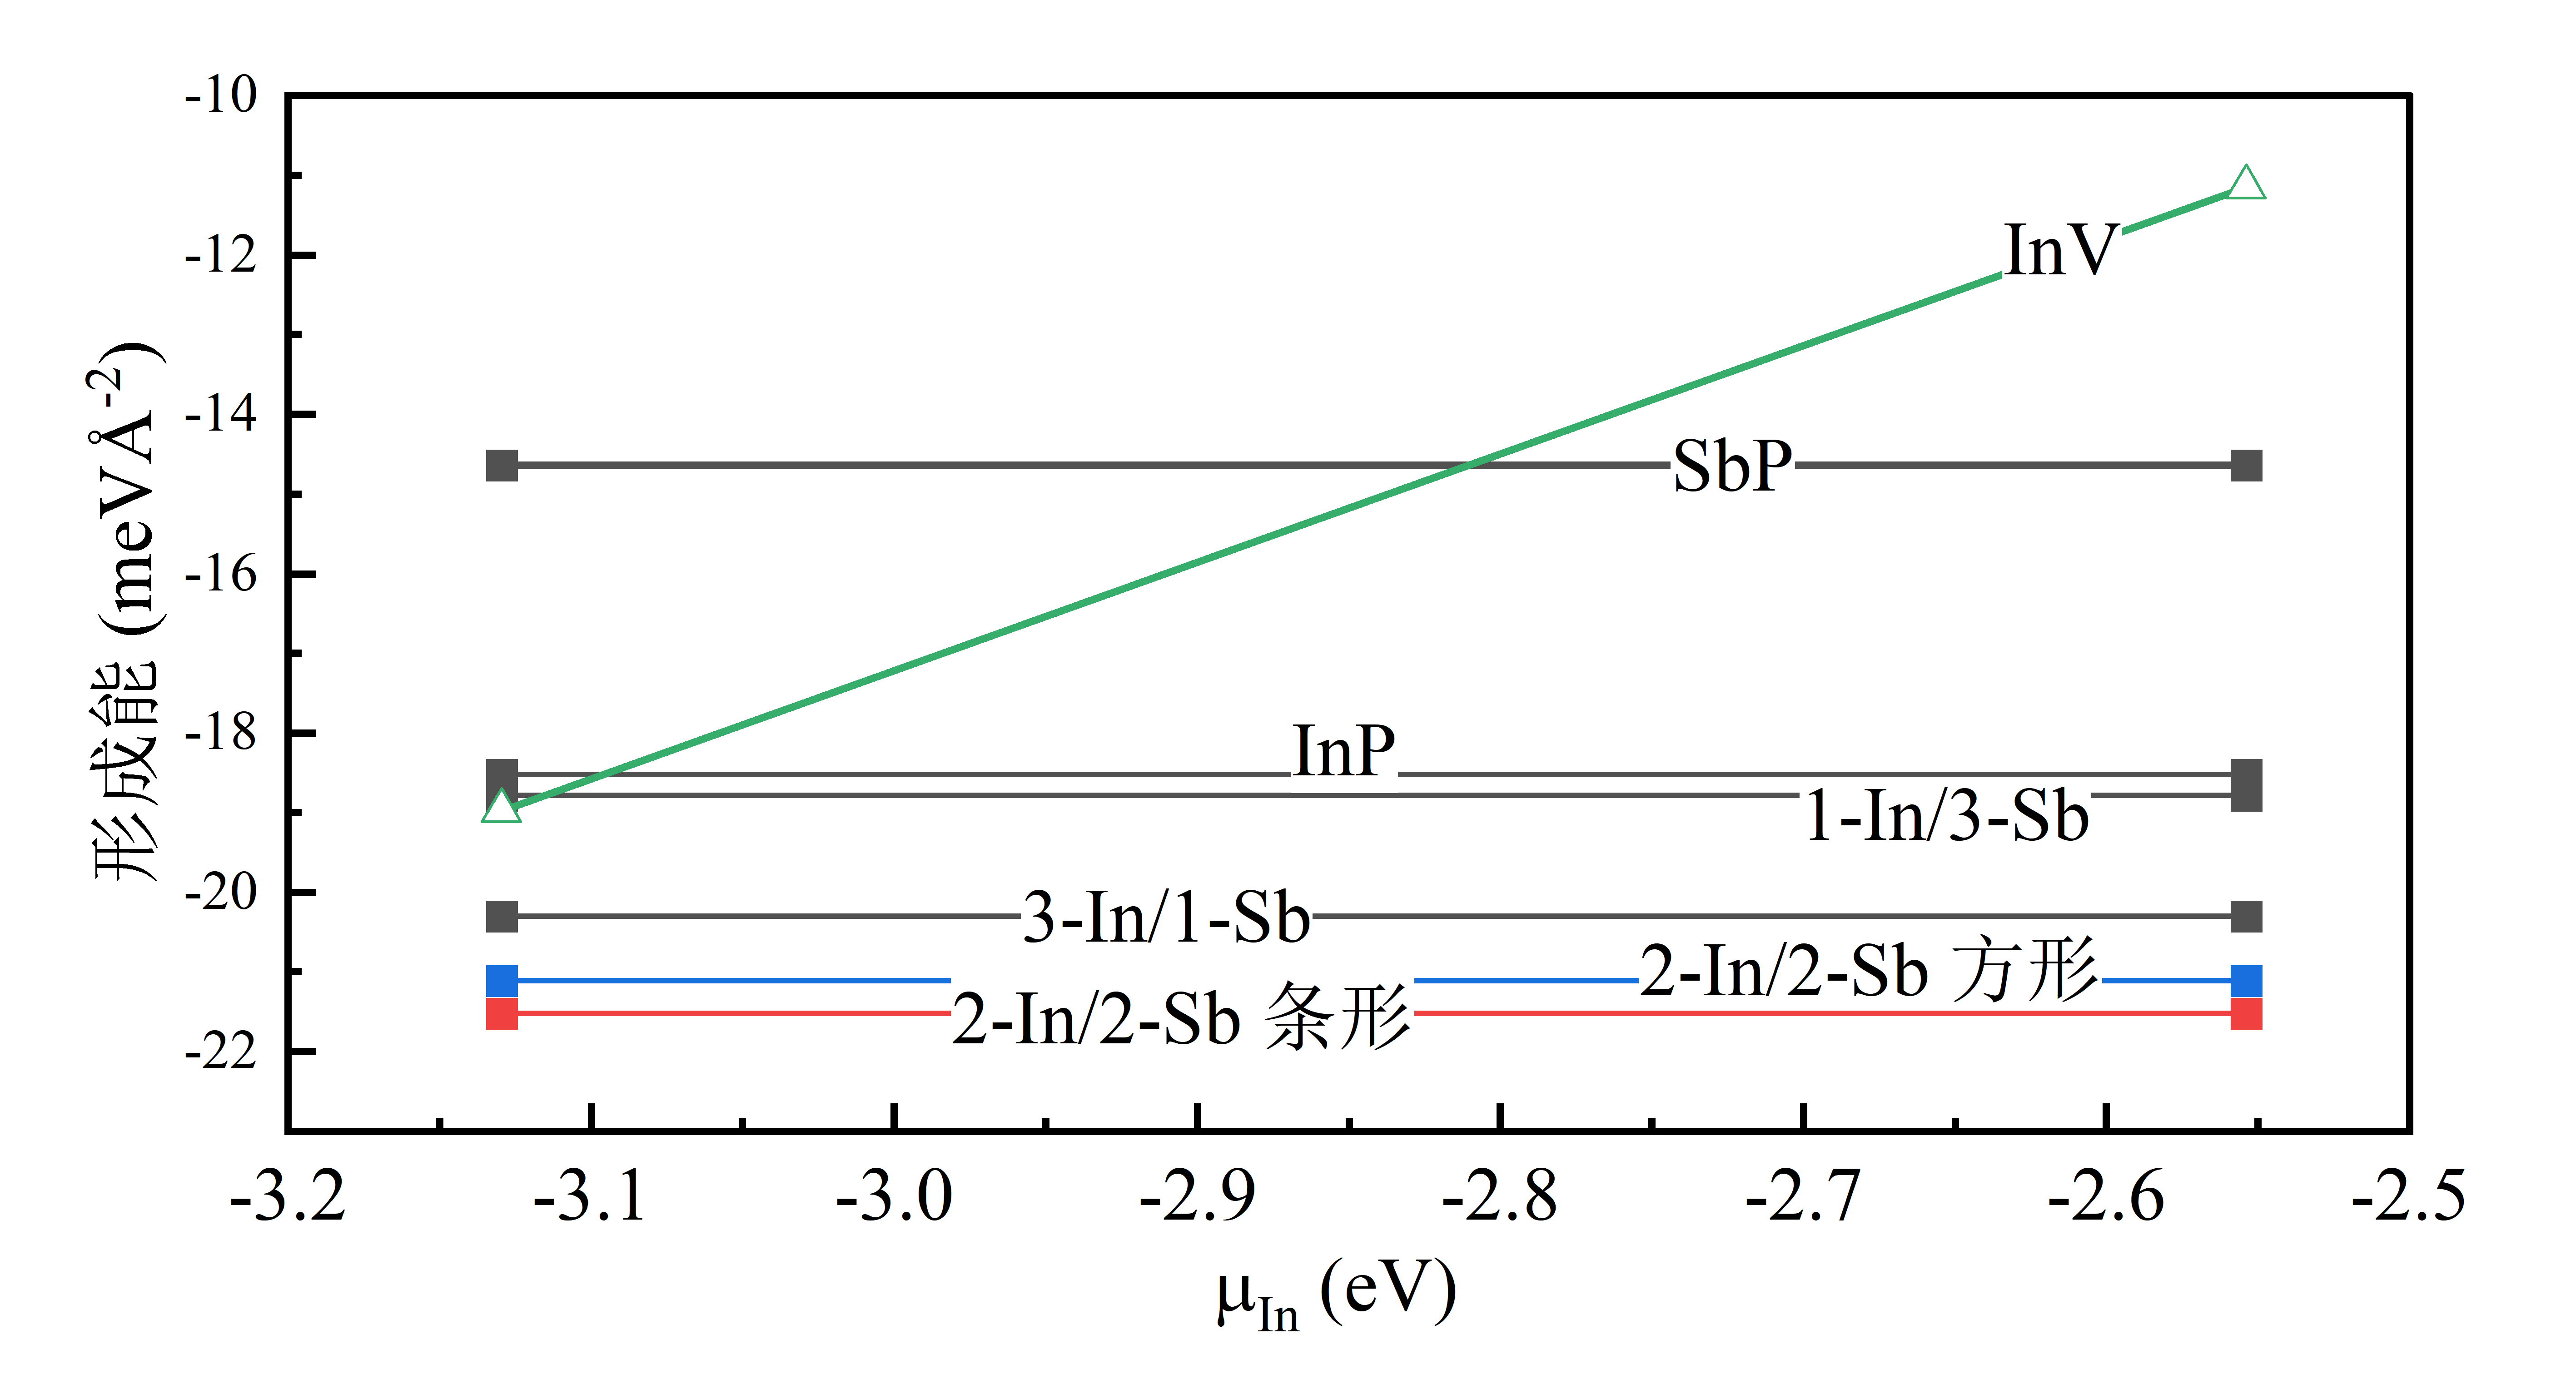
\includegraphics{pic/IS_DFT_1InSb_FlipVsInV.png}
    \caption{\cemb{Bi(001)}表面不同极性单层\cemb{InSb}和\cemb{In}空位重构层的形成能对比}
    \label{fig:IS_DFT_1InSb_FlipVsInV}
\end{figure}

此外,本文发现在B型\cemb{In2Sb1}第二层下方的\cemb{In}极性\cemb{InSb}在在原子优化后变为了\cemb{In}空位层。多余的\cemb{In}原子被挤入第二层的团簇之中,形成了包含三个\cemb{In}原子的\cemb{In}三聚体。本文同时检查了\cemb{In}空位的重构构型在单层\cemb{InSb}中的形成能情况。如图\ref{fig:IS_DFT_1InSb_FlipVsInV}所示,只有在接近纯\cemb{Sb}环境的情况下,在\cemb{Bi(001)}表面\cemb{In}空位的形成能略低于\cemb{In}极性单层和\InSbMLpolar{1}{3}混合极性单层的形成能。随着生长环境中\cemb{In}原子浓度的上升,\cemb{In}原子的活性上升,环境中的\cemb{In}原子会倾向于填补\cemb{InSb}中的\cemb{In}空位,导致\cemb{In}空位的形成能也上升并且会超过\cemb{Sb}极性的单层\cemb{InSb}的形成能。

\begin{figure}[htb]
    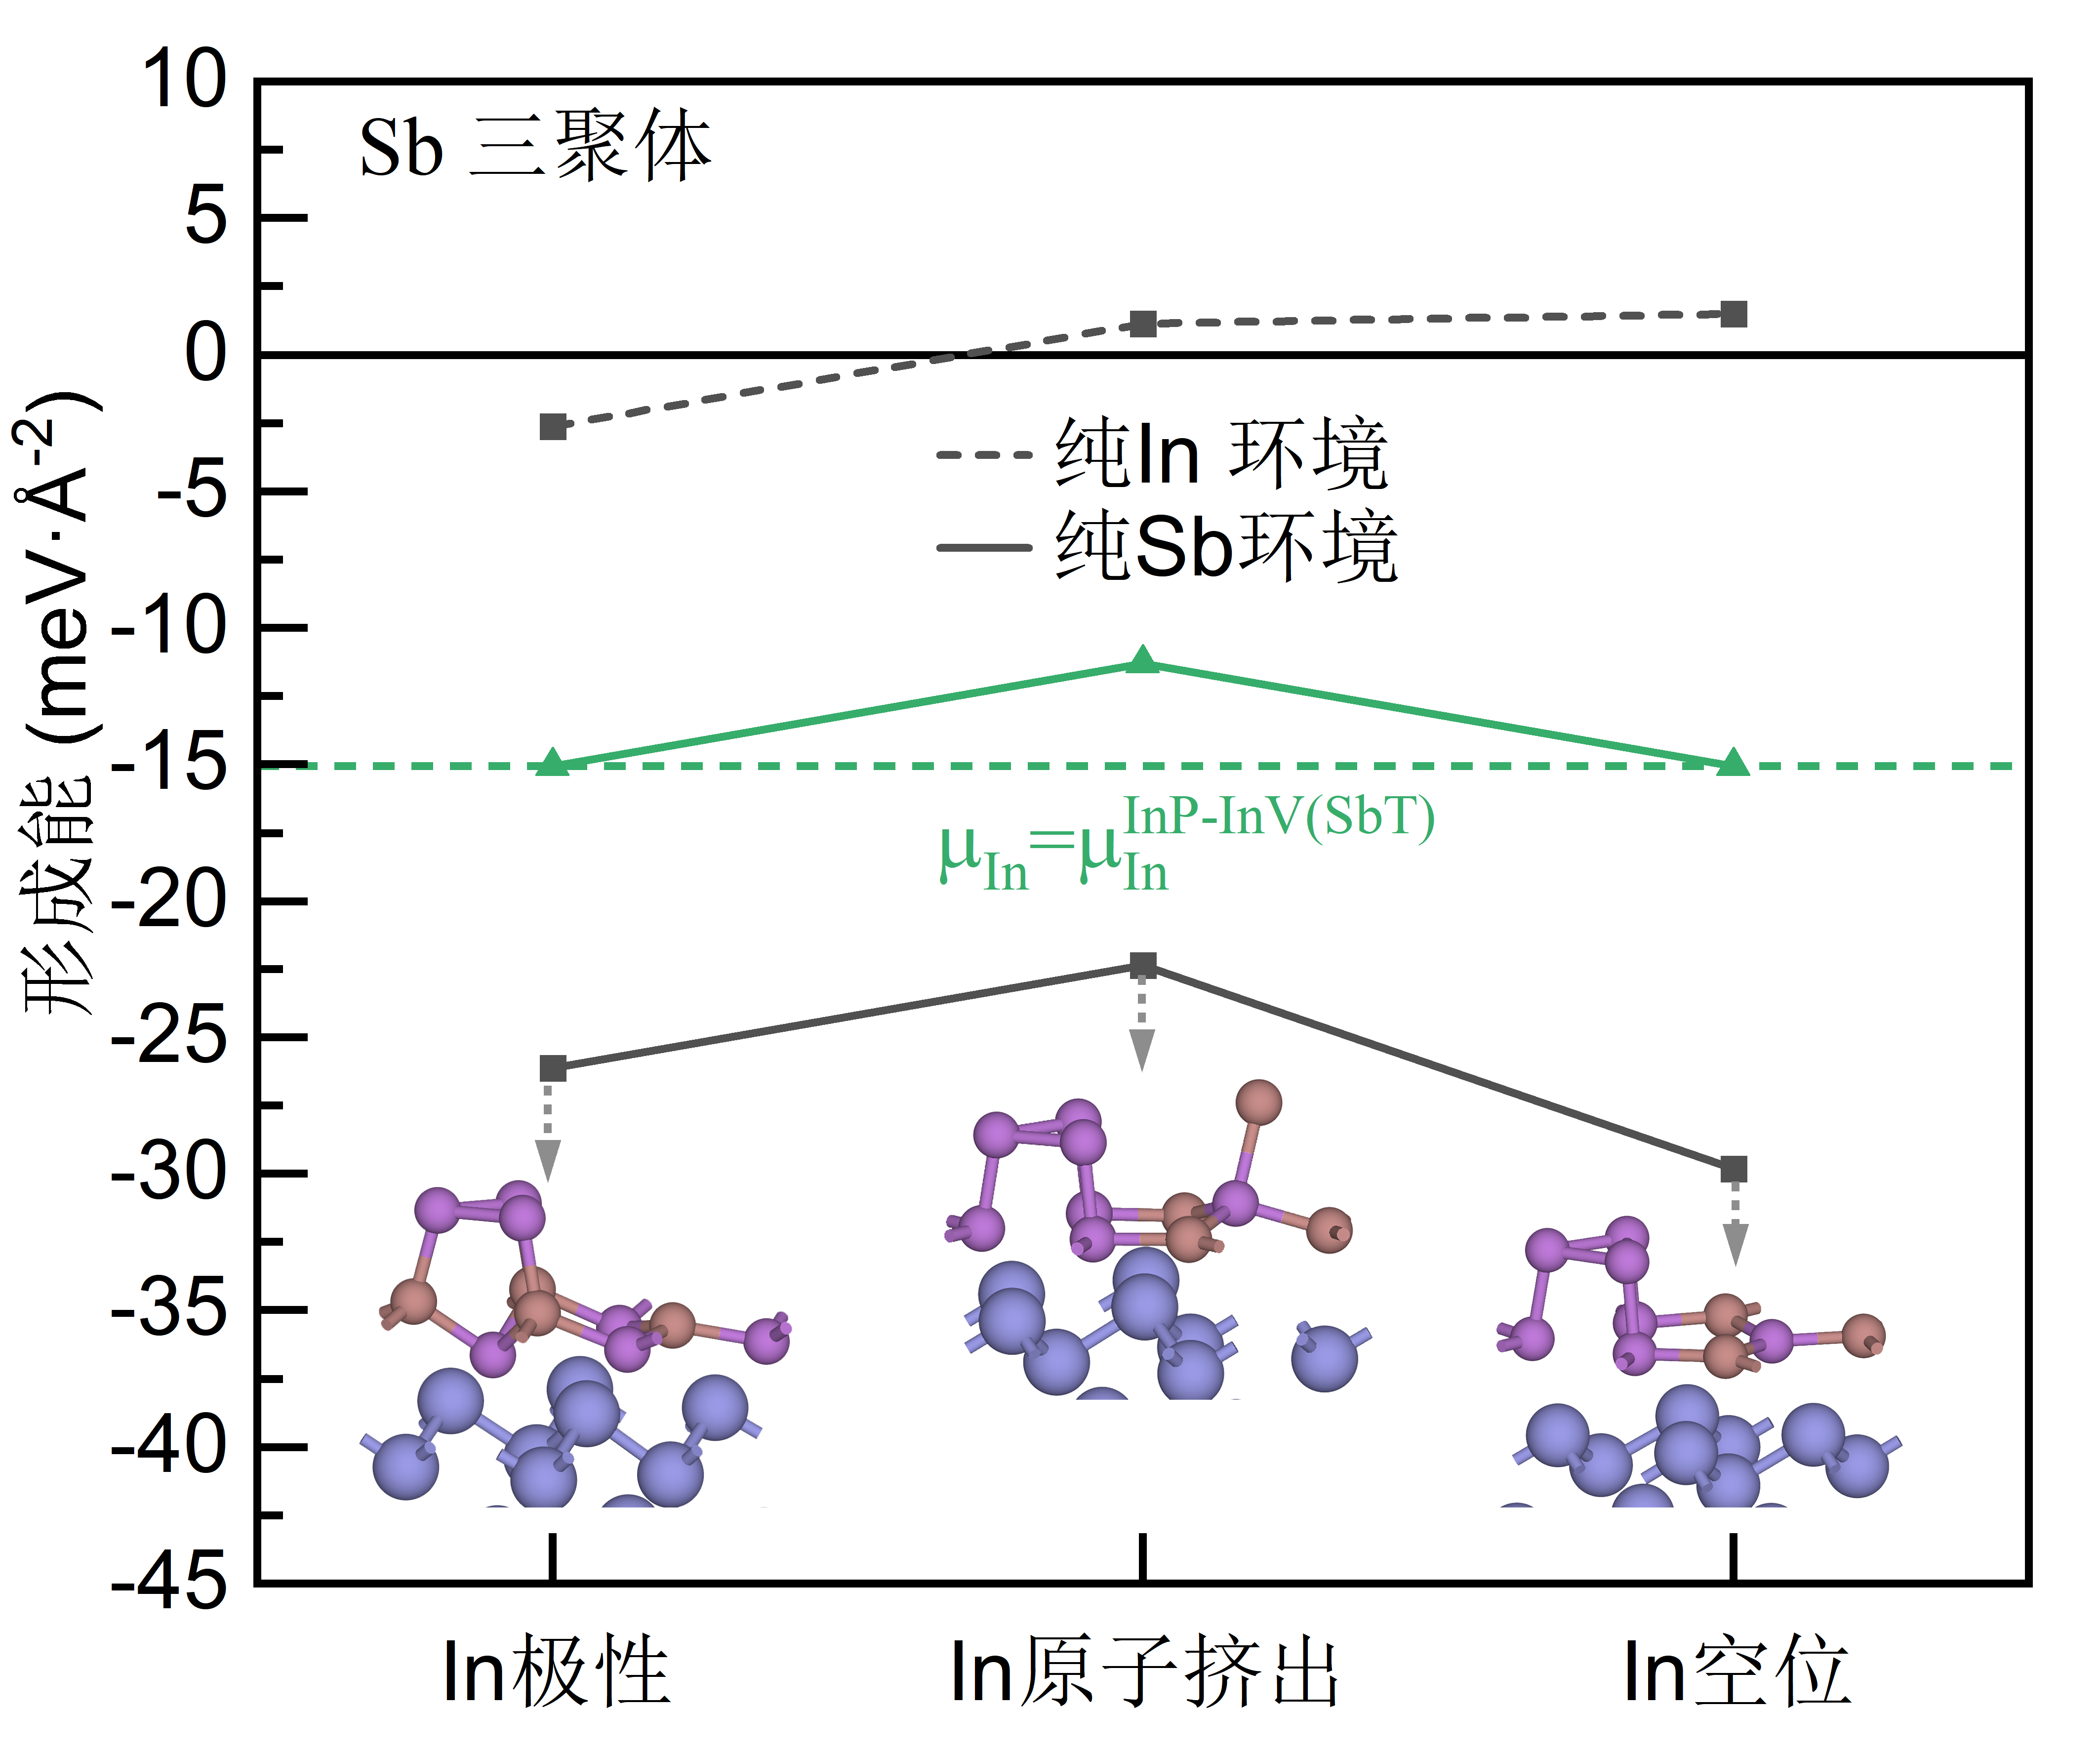
\includegraphics{pic/IS_DFT_2InSb_InPtoInV.png}
    \caption{\cemb{Sb}三聚体重构为第二层时,第一层\cemb{InSb}在\cemb{In}极性和\cemb{In}空位重构构型之间的转换过程。原子结构图中,\cemb{Bi}原子使用蓝色表示,\cemb{In}原子使用褐色表示,\cemb{Sb}原子使用紫色表示}
    \label{fig:IS_DFT_2InSb_InPtoInV}
\end{figure}

在\cemb{Sb}三聚体的和$\muVar{In}{}$的作用下,双层\cemb{InSb}中第一层的原子结构可以在\cemb{In}极性和\cemb{In}空位重构之间来回变换。在这个过程中需要将\cemb{In}极性\cemb{InSb}第一层中的一个\cemb{In}原子挤出原本的晶格位置。如图\ref{fig:IS_DFT_2InSb_InPtoInV}所示,当\cemb{In}极性\cemb{InSb}第一层中的一个\cemb{In}原子被挤出后,会停留在\cemb{InSb}的表面原本的$\TfourSite$形成独立的吸附原子。\cemb{InSb}单层在缺失了一个\cemb{In}原子之后形成了类似于\cemb{In}空位重构的平面形式。挤出的\cemb{In}原子会于第一层\cemb{InSb}中的\cemb{Sb}原子成键,将其略微拉出\cemb{In}空位重构所形成的平面。根据本文的计算,将\cemb{In}极性的\cemb{InSb}中的一个\cemb{In}原子挤出为吸附原子的反应为吸热反应,需要吸收约\SI{5}{\mievpas}的能量。

注意到从原子结构的角度看,\cemb{In}空位重构的原子结构可以由\cemb{Sb}三聚体重构表面继续吸附三个\cemb{In}原子和一个\cemb{Sb}原子形成。因此,在生长的过程中,\cemb{In}重构表面的第二层可能是从团簇阶段的\cemb{Sb}三聚体重构表面演化而来,并在\cemb{Sb}三聚体重构的第二层基础上进一步将第一层多晶态的\cemb{InSb}完全极化至\cemb{In}极性。因此,进一步考虑第一层\cemb{InSb}位\cemb{In}空位重构构型的情况,本文在图\ref{fig:IS_2Linsb_InVfirstlayer}中比较了当第二层\cemb{InSb}生长了\cemb{Sb}三聚体重构和\cemb{In}空位层后,第一层位\cemb{In}极性或者\cemb{In}空位层的形成能情况。对于以\cemb{Sb}三聚体重构作为第二层的双层\cemb{InSb},\cemb{In}极性第一层和\cemb{In}空位重构第一层的形成能非常接近。由于\cemb{In}空位重构的第一层缺少一个\cemb{In}原子,其在\cemb{Sb}浓度较高的生长环境中相比于\cemb{In}极性的第一层具有更低的形成能。而当生长环境中的\cemb{In}原子浓度升高后,\cemb{In}原子的活性上升,\cemb{In}极性的\cemb{InSb}第一层开始在形成能方面占据优势。在\cemb{Sb}三聚体结构的第二层下,\cemb{In}空位和\cemb{In}极性的第一层\cemb{InSb}的转变化学式$\muVar{In}{}$为$\muVar{In}{InP-InV\left(SbT\right)}=\SI{-2.86}{\electronvolt}$。

\begin{figure}[htb]
    \subfloat[]{
        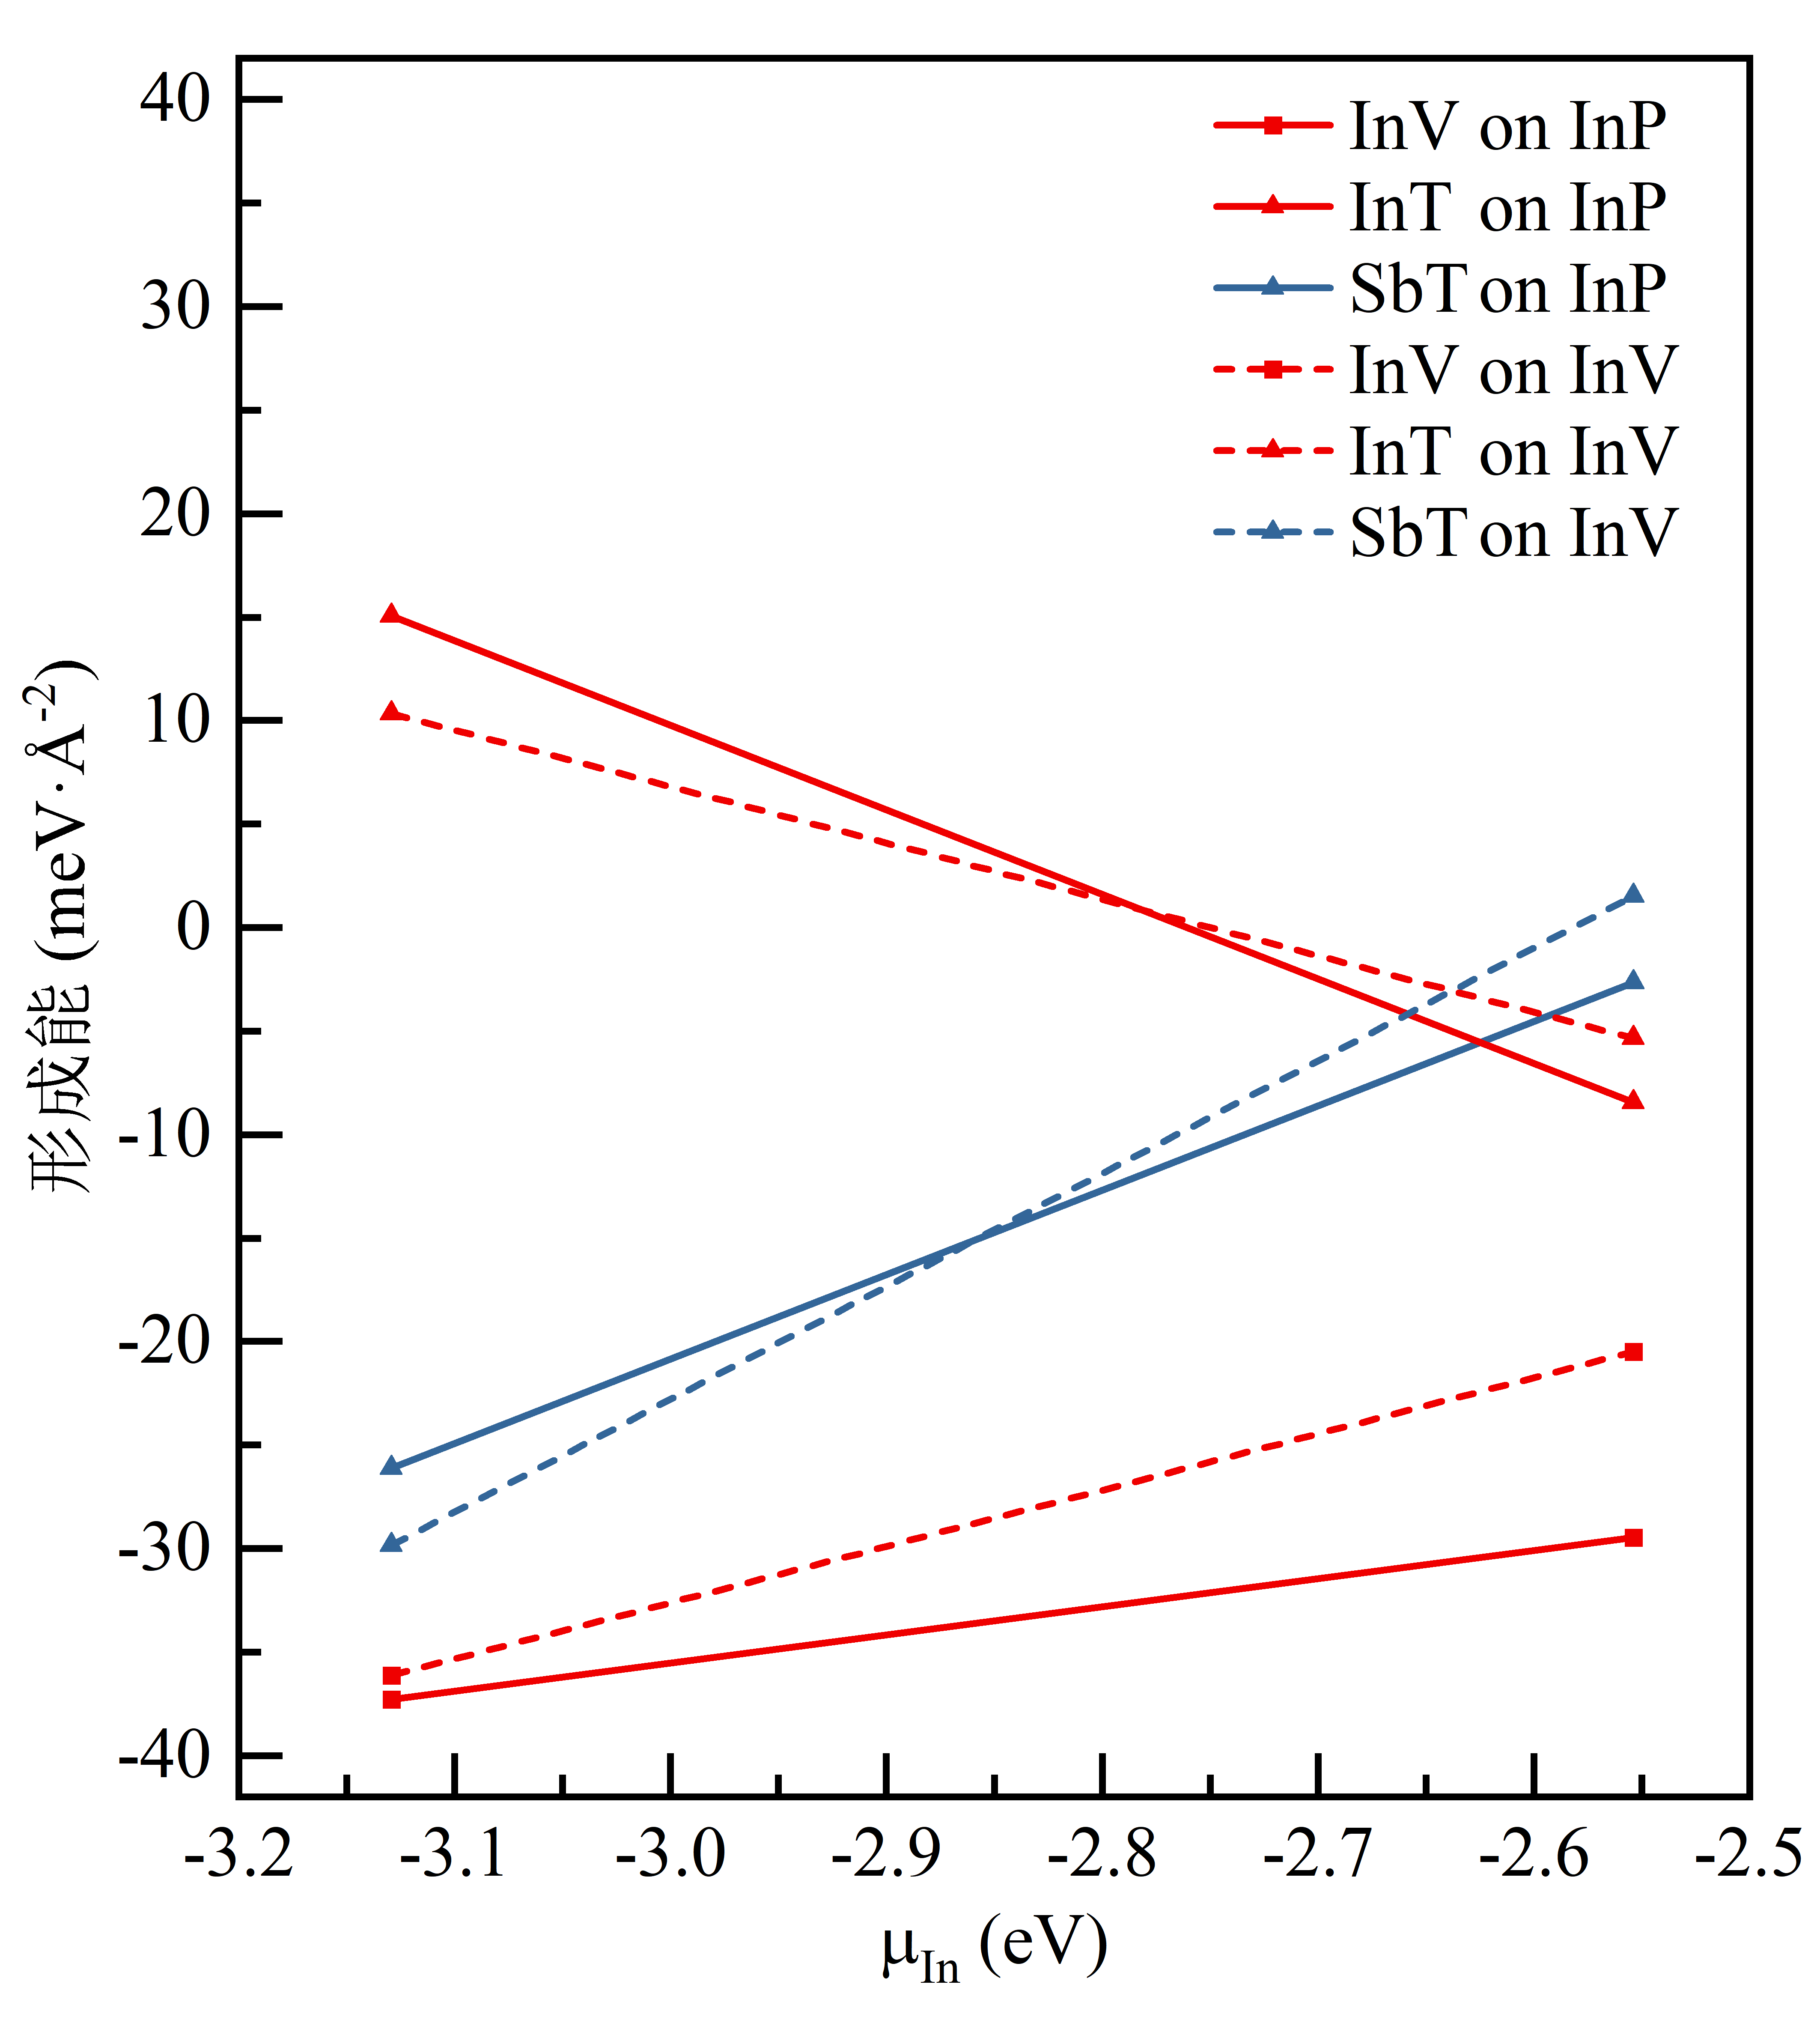
\includegraphics[width=0.55\textwidth]{pic/IS_DFT_2LInSb_SbT-InV-InT_InV-InP.png}
    }
    \begin{minipage}[b]{0.4\textwidth}
        \subfloat[]{
            \label{fig:IS_structure_SbTonInV}
            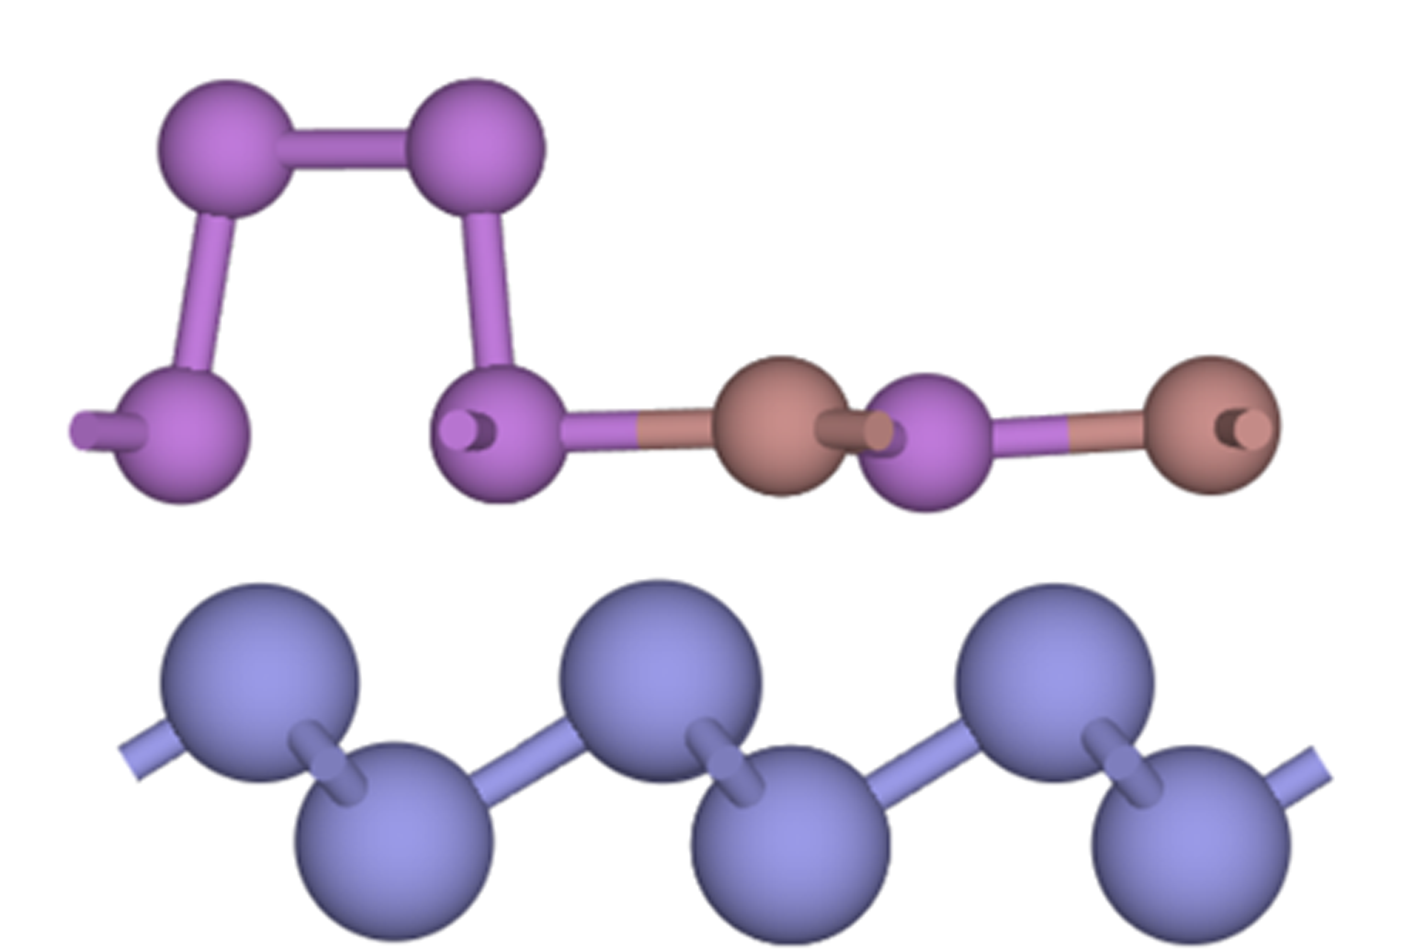
\includegraphics[width=0.9\textwidth]{pic/IS_structure_SbTonInV.png}
        }
        \newline
        \subfloat[]{
            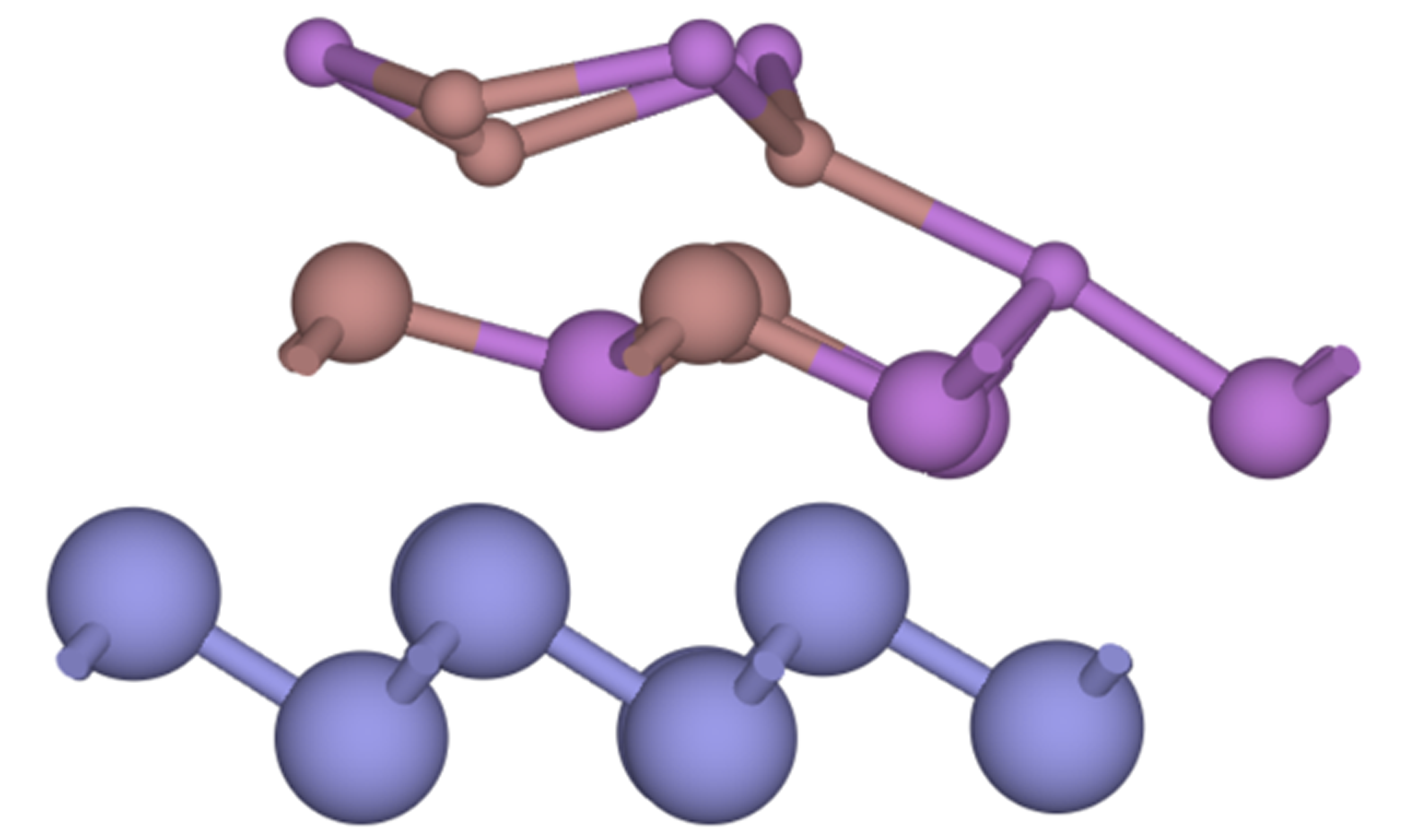
\includegraphics[width=0.9\textwidth]{pic/IS_structure_InVonInV.png}
        }
    \end{minipage}
    \caption{\cemb{Sb}三聚体层和\cemb{In}重构层在\cemb{In}极性和\cemb{In}空位层生长的形成能以及原子结构图。(a)形成能随$\muVar{In}{}$的变化情况;(b)\cemb{Sb}三聚体层\cemb{In}空位\cemb{InSb}上生长的结构图;(c)\cemb{In}空位层\cemb{In}空位\cemb{InSb}上生长的结构图。原子结构图中,\cemb{Bi}原子使用蓝色表示,\cemb{In}原子使用褐色表示,\cemb{Sb}原子使用紫色表示}
    \label{fig:IS_2Linsb_InVfirstlayer}
\end{figure}


而对于以\cemb{In}空位重构作为第二层的双层\cemb{InSb},可以发现在本文所考虑的$\muVar{In}{}$范围内,以\cemb{In}重构层为第二层比以\cemb{Sb}三聚体重构为第二层的双层\cemb{InSb}具有更低的形成能。同时,以\cemb{In}空位重构作为第一层\cemb{InSb}构型的形成能在最有优势的纯\cemb{Sb}极限环境下仍然不及\cemb{In}极性的构型稳定。因此,当双层\cemb{InSb}在生长的过程中,第二层的\cemb{InSb}由团簇阶段的三聚体生长为\cemb{In}空位重构层时,第一层的\cemb{In}空位构型会在第二层\cemb{In}空位重构层的作用下还原为\cemb{In}极性的构型。

考虑到第一层以混合极性为主的非静态\cemb{InSb}只能在\cemb{Sb}三聚体重构第二层的作用下转变为以\cemb{Sb}极性和\cemb{In}极性为主的多晶态双层\cemb{InSb}。同时在$\muVar{In}{}$的影响下,还会有部分第一层\cemb{InSb}会从\cemb{In}极性转变为以\cemb{In}空位重构的构型。而当更多的原子从生长气氛中沉积到单层\cemb{InSb}的表面,第二层\cemb{InSb}的生长阶段由以\cemb{Sb}三聚体为主的团簇阶段变为\cemb{In}空位表面重构阶段,不仅双层\cemb{InSb}的形成能得到了进一步的降低,第一层中\cemb{Sb}极性的表面也会在\cemb{In}空位表面重构的作用下进一步极化至\cemb{In}极性的构型,同时第一层中\cemb{In}空位也会在体系能量最低的作用下的被还原为\cemb{In}极性。

本文将\cemb{InSb}第二层从原子吸附到形成\cemb{In}空位表面重构层的生长序列随着生长环境\cemb{$\muVar{In}{}$}的变化绘制成了生长阶段相图(图\ref{fig:IS_DFT_stagePhase})。在原子吸附阶段,由于在\InSbMLpolar{2}{2} 条形单层\cemb{InSb}表面存在\cemb{Sb}原子和\cemb{In}原子都无法吸附的$\muVar{In}{}$区间(原子脱附区,相图中使用灰色表示)。在这个区间内,由于单层\cemb{InSb}表面原子的缺乏,在第二层\cemb{InSb}生长进入团簇的阶段无法直接形成形成\cemb{In_xSb_{3-x}}团簇。只有当一定数量的\cemb{Sb}原子在热涨落的作用下在\cemb{InSb}的表面聚集,克服表面原子脱附的趋势后才能形成\cemb{Sb}团簇降低形成能。

当环境中的$\muVar{In}{}$位于\cemb{Sb}原子的吸附区间时,生长环境中的\cemb{Sb}原子在混合极性的\cemb{InSb}单层表面沉积,形成\cemb{Sb}三聚体团簇并将第一层的\cemb{InSb}结构引导至\cemb{Sb}极性或者\cemb{In}极性。更低的$\muVar{In}{}$(更加接近纯\cemb{Sb}极限环境)还可能使第一层中的某些\cemb{In}原子脱离,在第一层\cemb{InSb}中形成\cemb{In}缺陷($\muVar{In}{}\leqslant \muVar{In}{InP-InV\left(SbT\right)}$)。

\begin{figure}[!htb]
    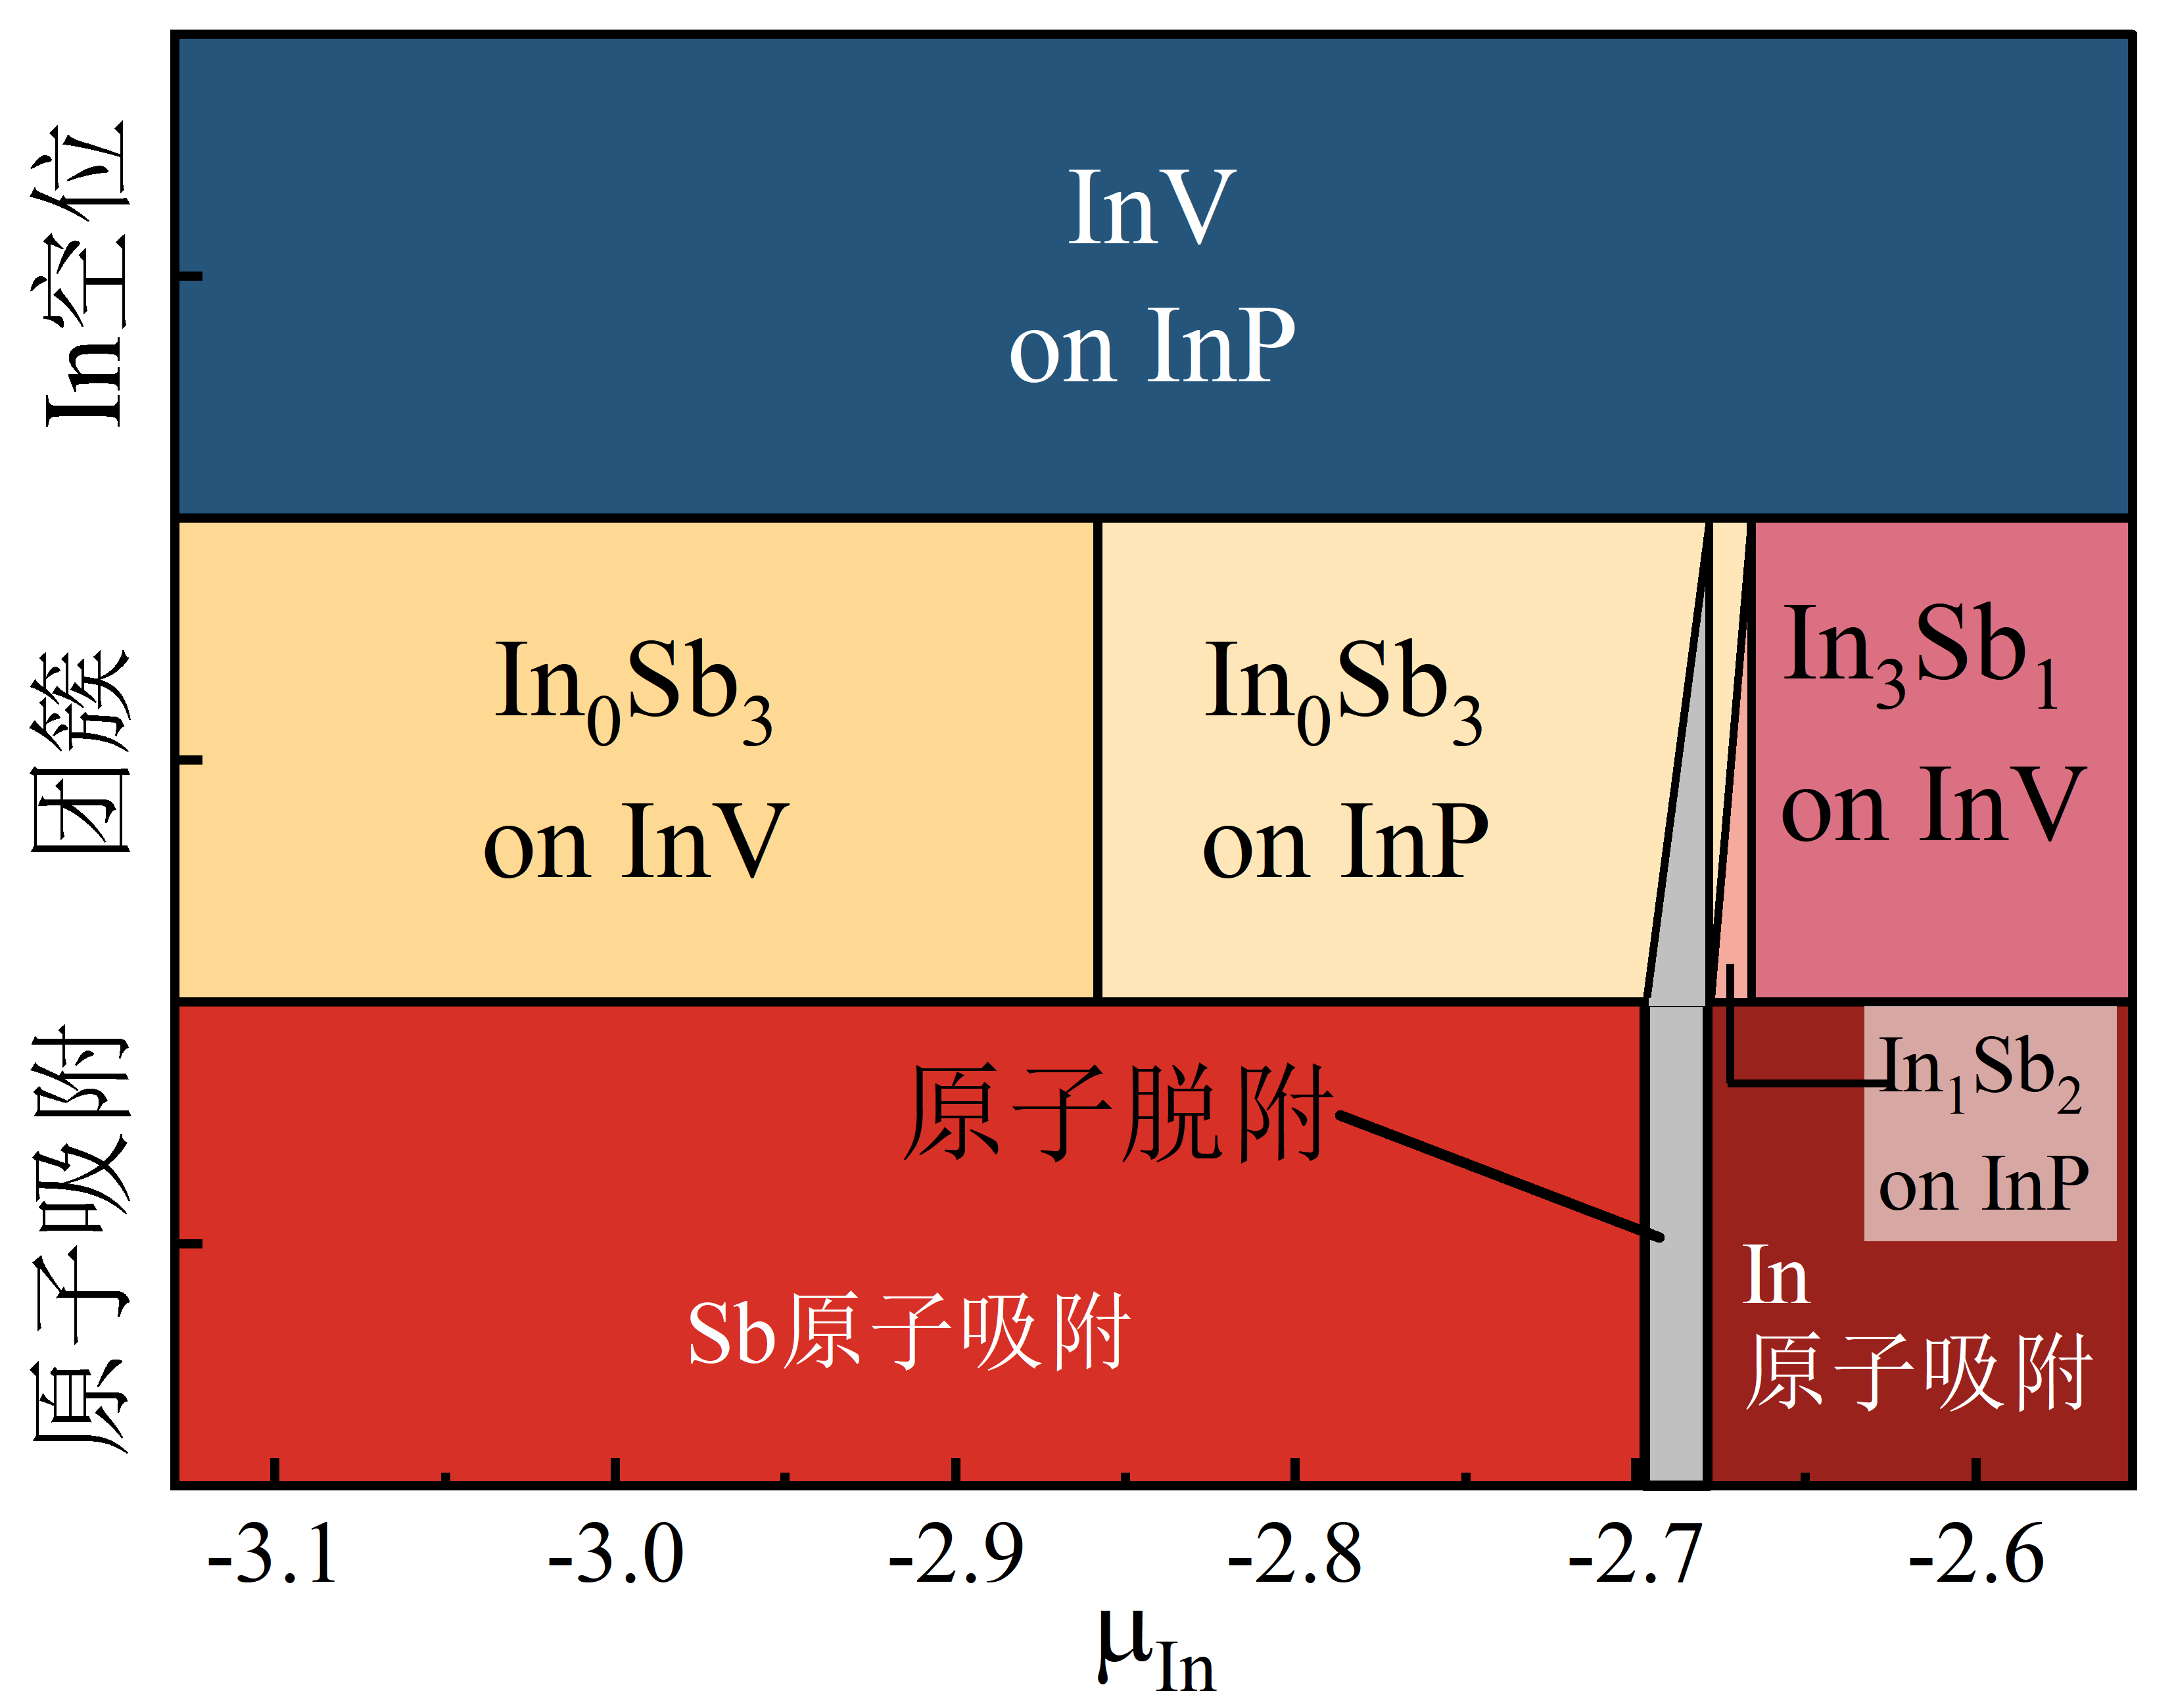
\includegraphics{pic/IS_DFT_stagePhase.png}
    \caption{双层\cemb{InSb}不同生长阶段的自极化相图}
    \label{fig:IS_DFT_stagePhase}
\end{figure}

在$\muVar{In}{}$取值的另一边,\cemb{In}原子吸附区的开端,由于缺乏\cemb{Sb}原子,无法在单层的\cemb{InSb}直接形成\cemb{Sb}三聚体团簇。生长环境中的\cemb{Sb}原子只能借助已吸附的\cemb{In}原子,形成\cemb{In1Sb2}团簇作为中间态。经过进一步的结构演化后,\cemb{In1Sb2}团簇中的\cemb{In}原子被环境中的\cemb{Sb}原子替代,形成更加稳定的\cemb{Sb}三聚体团簇。当$\muVar{In}{}$的取值更加接近纯\cemb{In}极限环境时,在\cemb{In}极性表面形成\cemb{Sb}三聚体的形成能会高于在\cemb{In}空位重构的第一层表面形成\cemb{In3Sb1}团簇的能量。在这种情况下,第二层\cemb{InSb}以\cemb{In3Sb1}团簇的形式存在,并且会将第一层\cemb{InSb}的结构转化成类似于\cemb{In}空位重构的构型。


随着生长的继续进行,更多环境中的\cemb{In}原子和\cemb{Sb}原子参与到第二层\cemb{InSb}的生长之中,使得第二层\cemb{InSb}的结构向\cemb{In}空位表面重构转化。\cemb{In}空位表面重构在第二层\cemb{InSb}的形成同时也驱使第一层\cemb{InSb}的构型转变为统一的\cemb{In}极性,完成双层\cemb{InSb}的自极化过程。

\subsection{双层\cemb{InSb}的极性演化}

在上一章中,本文对于双层\cemb{InSb}生长的极化过程的研究集中在第二层\cemb{InSb}的覆盖率为1的情况。在本章中,通过引入不同覆盖度的第二层\cemb{InSb},可以进一步探究\cemb{InSb}极化过程和沉积时间之间的关系。在本章中,本文将双层\cemb{InSb}的极化过程分为三个阶段\chinesecolon 第一个阶段为非晶态阶段(无第二层);第二个阶段为多晶阶段(第二层为\cemb{Sb}三聚体重构);第三个阶段为\cemb{In}极性阶段(第二层为\cemb{In}空位重构)。对于第一层的\cemb{InSb},本文选用\InSbMLpolar{2}{2} 条形构型和\cemb{In}极性(\InSbMLpolar{4}{0})构型来表示非极化的和在第二层\cemb{InSb}作用下极化的第一层\cemb{InSb}。对于沉积时间,本文假设生长环境中的原子在单层\cemb{InSb}的表面沉积是连续、均匀的。因此本文使用在单层\cemb{InSb}表面沉积、形成第二层\cemb{InSb}的吸附原子数量$\NumOfAdatom$来代表第二层\cemb{InSb}的沉积生长时间。同时,为了对具有不同覆盖度不同覆盖度的第二层的双层\cemb{InSb}进行计算,如图\ref{fig:IS_diagram_2Linsb_partial}所示,本文将模拟原胞扩大到$4 \times 4$\cemb{InSb}切片模型,并将整个\cemb{InSb}单层区域的表面分成四个独立的第二层\cemb{InSb}生长区块,可以提供以$1/ 4$覆盖率为间隔的部分覆盖\cemb{InSb}第二层生长。


\begin{figure}[h]
    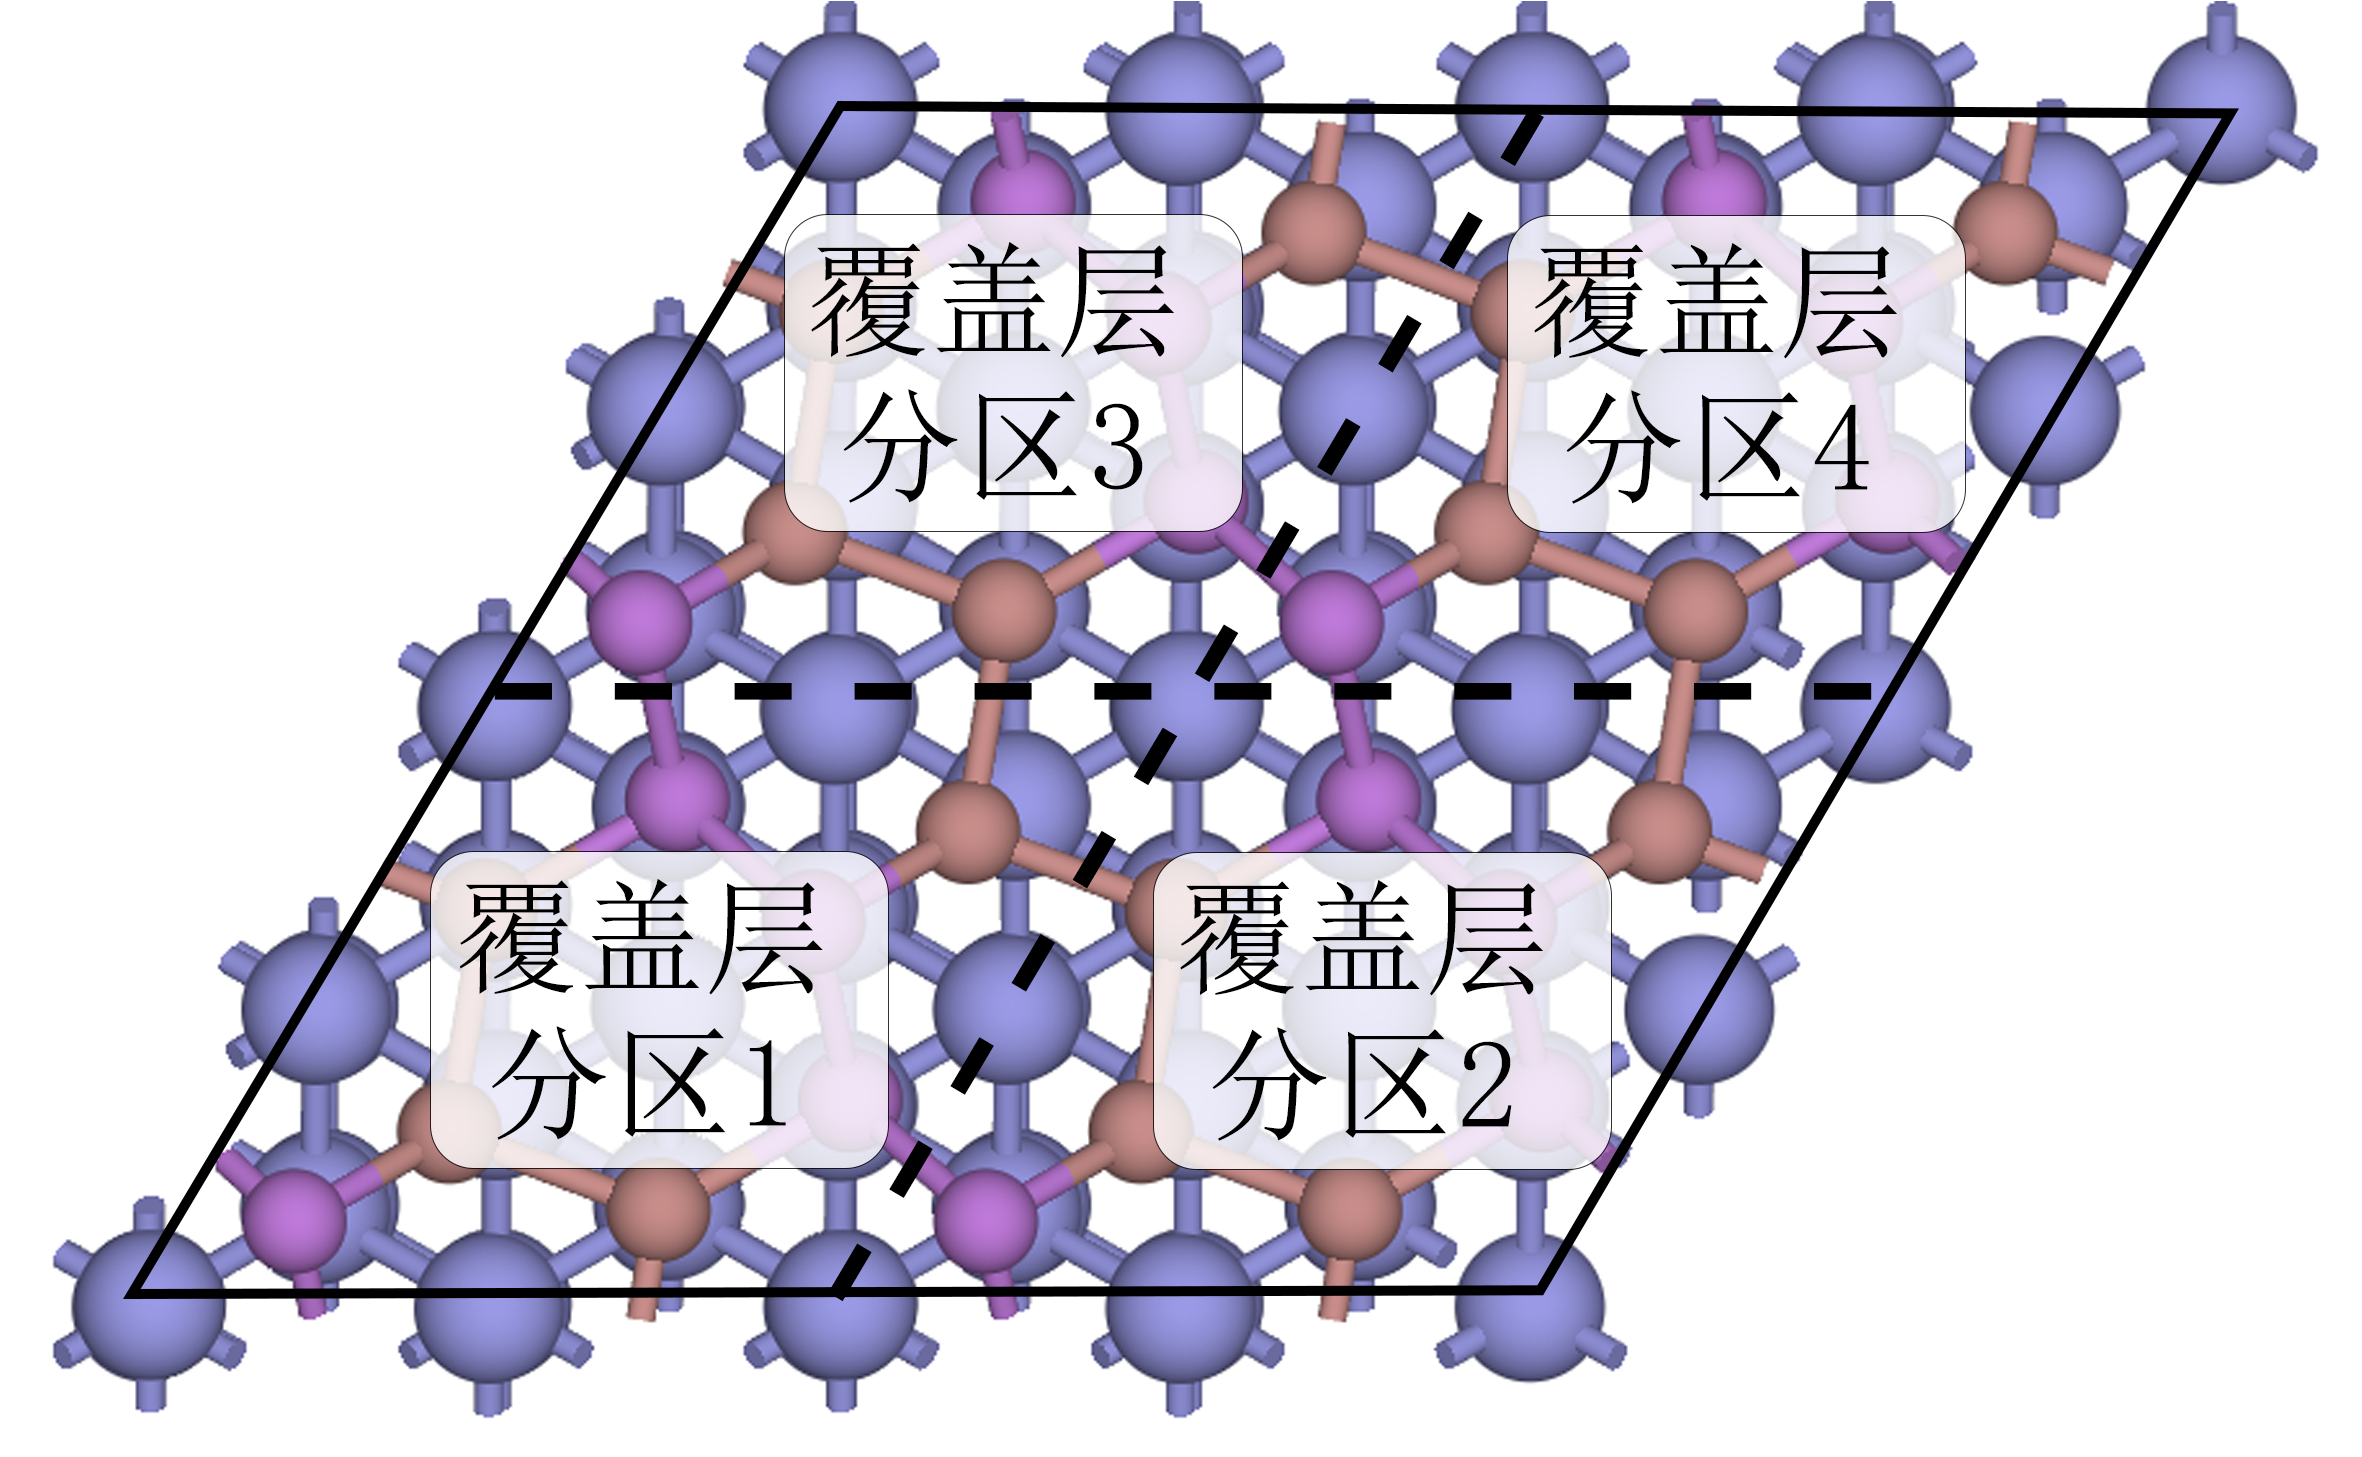
\includegraphics{pic/IS_diagram_2Linsb_partial.png}
    \caption{$4 \times 4$\cemb{InSb}切片模型中四个独立的第二层\cemb{InSb}生长区块示意图}
    \label{fig:IS_diagram_2Linsb_partial}
\end{figure}

对于双层\cemb{InSb}的生长,在本章中本文将关注重点放在第二层为\cemb{Sb}三聚体表面重构构型和\cemb{In}空位表面重构对于第一层\cemb{InSb}极性的转化过程。为了减小搜索范围,当第二层为\cemb{Sb}三聚体重构时,第一层\cemb{InSb}中\cemb{In}空位的形成仅通过$\muVar{In}{}$与转变点$\muVar{In}{InP-InV\left(SbT\right)}$的关系进行判定。

本文使用$C_{N_{\rm InV}\rm InV}^{N_{\rm SbT}\rm SbT}$来表示非满覆盖二层生长的双层\cemb{InSb}的原子构型。其中$C$是已生长的第二层\cemb{InSb}的总覆盖度,$N_{\rm InV}$和$N_{\rm SbT}$代表\cemb{In}空位重构和\cemb{Sb}三聚体重构在模拟晶胞中占据的区块的数量。

\begin{figure}[htb]
    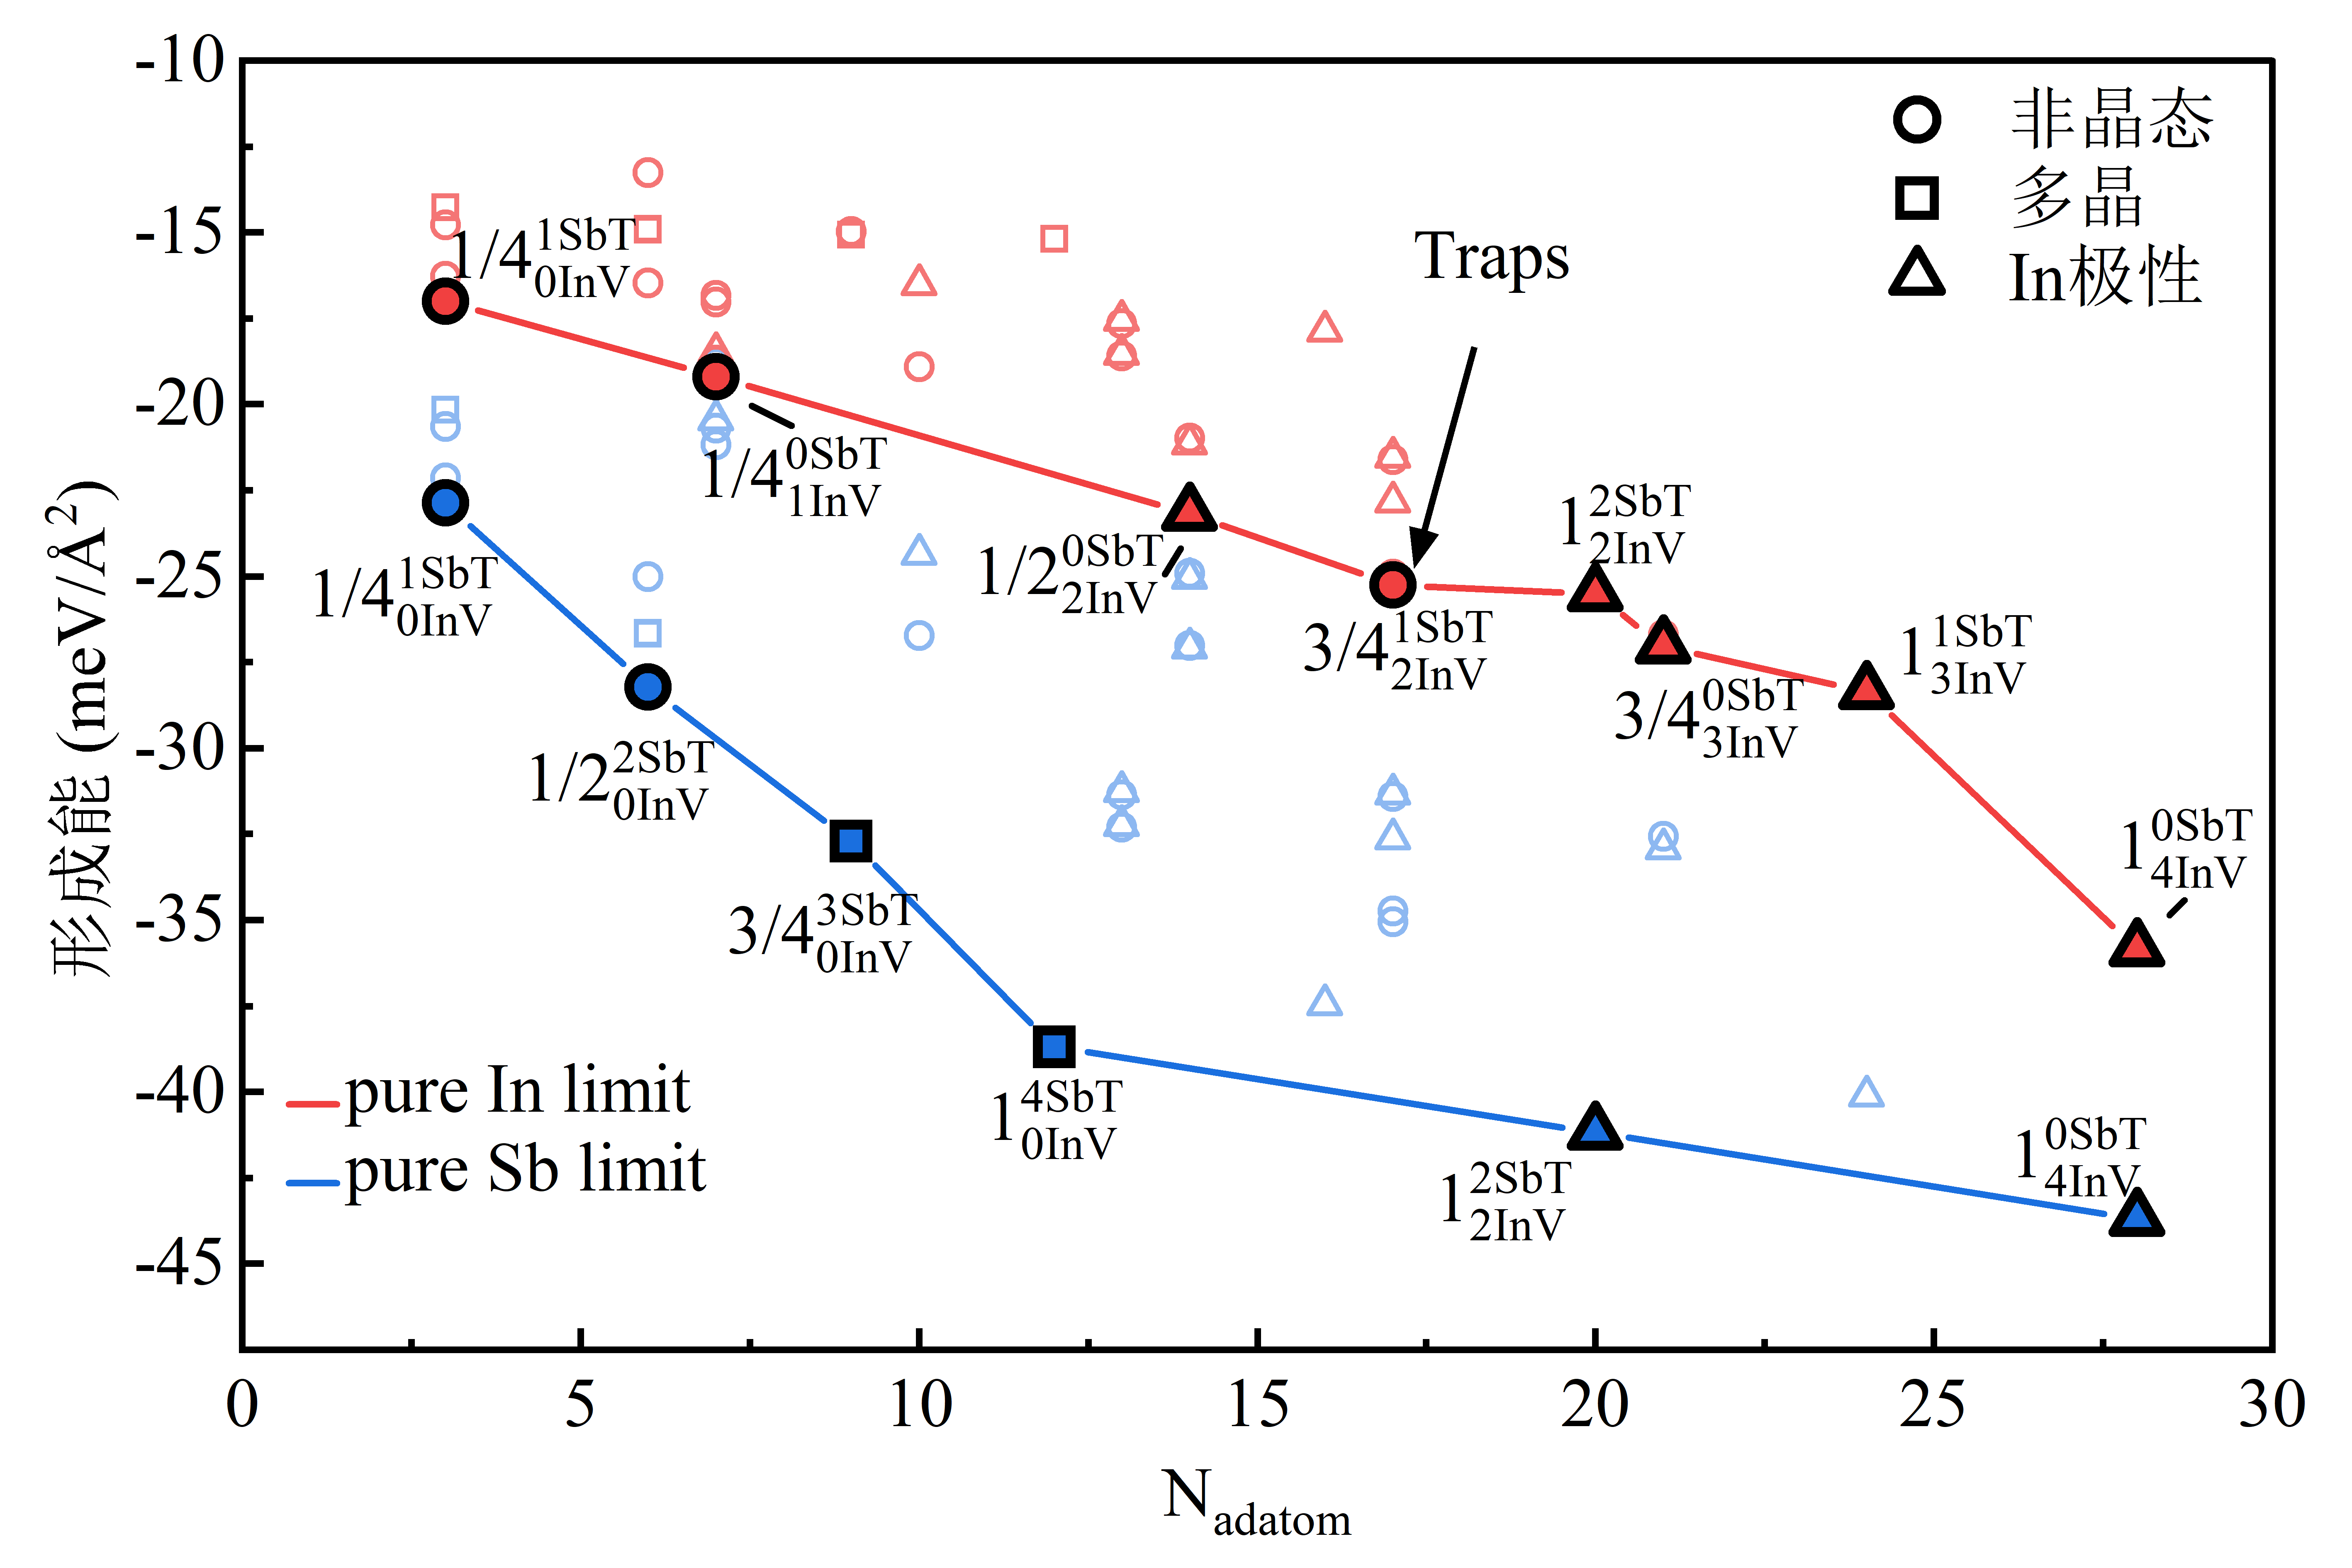
\includegraphics{pic/IS_DFT_2LInSb_partEnergy.png}
    \caption{在纯\cemb{Sb}和纯\cemb{In}极限的生长气氛环境下双层\cemb{InSb}随着沉积时间增长的形成能分布和极性演化过程}
    \label{fig:IS_DFT_2LInSb_partEnergy}
\end{figure}

在图\ref{fig:IS_DFT_2LInSb_partEnergy}中,本文绘制了在纯\cemb{Sb}和纯\cemb{In}极限的生长环境下双层\cemb{InSb}随着沉积时间增长的形成能分布和极性演化过程。在纯\cemb{Sb}环境中,\cemb{Sb}三聚体表面重构拥有非常高的形成能能量优势。随着沉积原子数的上升,越来越多的\cemb{Sb}三聚体表面重构在单层\cemb{InSb}的表面生长,并且将各自下方区域的第一层\cemb{InSb}局部得转变为\cemb{In}极性或者\cemb{Sb}极性的结构。

第一层\cemb{InSb}的首次极化开始于$\CNinNsb{3}{4}{0}{3}$。在$\CNinNsb{3}{4}{0}{3}$构型的双层\cemb{InSb}中,最后一块未生长第二层\cemb{InSb}的区块在边界能的作用下自发转变成与周围相同极化的晶态结构,使得整个双层\cemb{InSb}在覆盖度为$\frac{3}{4}$的\cemb{Sb}三聚体第二层的作用下被极化为以\cemb{In}极性和\cemb{Sb}极性为主的多晶构型。在纯\cemb{Sb}极限环境中高活性的\cemb{Sb}原子不仅促进了\cemb{Sb}三聚体重构第二层的生长,而且还阻止了以\cemb{In}空位重构为构型的第二层的形成。根据本文的形成能计算,包含6个吸附原子的$\CNinNsb{1}{2}{0}{2}$构型的形成能低于包含7个吸附原子的$\CNinNsb{1}{4}{1}{0}$。因此在生长了覆盖率为$\frac{1}{2}$的\cemb{Sb}三聚体重构第二层后,生长气氛中的\cemb{In}原子和\cemb{Sb}原子并不会在已经形成的\cemb{Sb}三聚体团簇的基础上继续生长出\cemb{In}空位重构,而是直接在未生长第二层的表面生长\cemb{Sb}三聚体重构第二层,从而形成能量更低的$\CNinNsb{3}{4}{0}{3}$构型的双层\cemb{InSb}。

\begin{figure}[htb]
    \subfloat[]{
        \includegraphics{pic/IS_structure_partical_1-2_0-2.png}
        \label{fig:IS_structure_partical_1-2_0-2}
    }
    \subfloat[]{
        \includegraphics{pic/IS_structure_partical_1-2_2-0.png}
        \label{fig:IS_structure_partical_1-2_2-0}
    }\\[-1ex]
    \subfloat[]{
        \includegraphics{pic/IS_structure_partical_3-4_0-3.png}
        \label{fig:IS_structure_partical_3-4_0-3}
    }
    \subfloat[]{
        \includegraphics{pic/IS_structure_partical_1-1_2-2.png}
        \label{fig:IS_structure_partical_1-1_2-2}
    }
    \caption{非满覆盖二层生长的双层\cemb{InSb}的原子构型。(a)$\CNinNsb{1}{2}{0}{2}$;(b)$\CNinNsb{1}{2}{2}{0}$,(c)$\CNinNsb{3}{4}{0}{3}$,(d)$\CNinNsb{1}{1}{1}{2}$。原子结构图中,\cemb{Bi}原子使用蓝色表示,\cemb{In}原子使用褐色表示,\cemb{Sb}原子使用紫色表示}
    \label{fig:IS_structure_partical_1}
\end{figure}

同时,包含9个吸附原子的$\CNinNsb{3}{4}{0}{3}$构型的形成能也低于包含10个吸附原子的$\CNinNsb{1}{2}{1}{1}$构型。因此在生长了覆盖率$\frac{1}{3}$的\cemb{Sb}三聚体重构的第二层后,\cemb{In}空位第二层同样无法在三聚体重构的基础上生成。直到生长了满覆盖的\cemb{Sb}三聚体重构后,包含12个吸附原子的$\CNinNsb{1}{1}{0}{4}$的形成能低于包含13个吸附原子的$\CNinNsb{3}{4}{1}{2}$、包含14个吸附原子的$\CNinNsb{1}{2}{2}{0}$、包含16个吸附原子的$\CNinNsb{1}{1}{1}{3}$、包含17个吸附原子的$\CNinNsb{3}{4}{2}{1}$。在跳过了这四个构型后,在纯\cemb{Sb}极限环境下的$\CNinNsb{1}{1}{0}{4}$构型倾向于直接生成更加稳定的$\CNinNsb{1}{1}{2}{2}$,包含20个吸附原子。$\CNinNsb{1}{1}{2}{2}$构型的形成同时在\cemb{In}空位重构的作用下,第一层\cemb{InSb}的被极化为\cemb{In}极性,完成双层\cemb{InSb}的极化过程。继续吸附生长环境中更多的原子可以形成满覆盖的\cemb{In}空位重构第二层,进一步降低\cemb{In}极性第二层的形成能,提升极化水平。

在纯\cemb{In}环境中,环境中的\cemb{Sb}原子很难在单层的\cemb{InSb}表面沉积,同时较高的$\muVar{In}{}$取值也导致形成\cemb{Sb}三聚体重构第二层的形成能较大。在这种情况下,随着生长过程而吸附在单层\cemb{InSb}表面的原子更倾向于直接形成\cemb{In}空位的第二层($\CNinNsb{1}{4}{1}{0}$),同时也将对应区块下的第一次层\cemb{InSb}局域地极化成\cemb{In}极性地构型。在聚集了14个吸附原子后,\cemb{InSb}单层的表面形成了覆盖率为$\frac{1}{2}$的\cemb{In}空位重构第二层。在这个过程中,双层\cemb{InSb}的极化过程直接跳过了多晶的步骤,$\CNinNsb{1}{2}{2}{0}$结构的第二层将未覆盖第二层的区域一并转变为了\cemb{In}极性的构型。在这种情况下,未覆盖第二层的单层\cemb{InSb},由于不同极性之间过高的晶界能,被迫与另邻位的被第二层所极化区域保持同样的极性构造,以保持形成能的最小化。

虽然早早得完成了全区域第一层向\cemb{In}极性结构的转变,但在$\CNinNsb{1}{2}{2}{0}$结构的第二层下,全\cemb{In}极性的第一层的形成能仅比包含非晶态的第一层的形成能高\SI{0.07}{\mievpas}。如此小的差距并不能保证双层\cemb{InSb}能够在热动能的影响下继续保持\cemb{In}极性的状态。进一步的计算表明,$\CNinNsb{1}{2}{2}{0}$结构继续吸附气氛中的三个\cemb{Sb}原子后,会在第二层中形成$\CNinNsb{3}{4}{2}{1}$结构。这个结构的产生不仅破坏了的原本规整的第二层\cemb{InSb}的晶格,而且还会在双层\cemb{InSb}的极化过程中成为一个陷阱步骤。使得原本在$\CNinNsb{1}{2}{2}{0}$结构的第二层下完成极化的\cemb{In}极性双层\cemb{InSb}转变为非晶态的构型。要越过$\CNinNsb{3}{4}{2}{1}$结构导致的陷阱步骤,需要进一步在单层\cemb{InSb}的表面上沉积原子,使得第二层的覆盖率达到1,形成$\CNinNsb{1}{1}{2}{2}$结构。

在$\CNinNsb{1}{1}{2}{2}$结构的第二层下,第一层\cemb{InSb}的结构到\cemb{In}极性的状态,但$\CNinNsb{1}{1}{2}{2}$结构下\cemb{In}极性的双层\cemb{InSb}的形成能只比陷阱步$\CNinNsb{3}{4}{2}{1}$结构下非晶态的双层\cemb{InSb}的形成能低\SI{0.27}{\mievpas}。因此只靠形成$\CNinNsb{1}{1}{2}{2}$结构的第二层并不能保证双层\cemb{InSb}的再次完全极化。为了进一步巩固极化的成果,需要吸附生长环境中更多的原子,计算显示\cemb{In}空位重构在第二层的覆盖率越大,\cemb{In}极性的双层\cemb{InSb}的形成能相对于非晶态陷阱步的优势就越大。在$\CNinNsb{1}{1}{4}{0}$结构的第二层下,\cemb{In}极性的双层\cemb{InSb}的形成能比陷阱步$\CNinNsb{3}{4}{2}{1}$结构下非晶态的形成能低大约\SI{10.61}{\mievpas}。

\begin{figure}[!b]
    \subfloat[]{
        \includegraphics{pic/IS_structure_partical_1-4_1-0.png}
        \label{fig:IS_structure_partical_1-4_1-0}
    }
    \subfloat[]{
        \includegraphics{pic/IS_structure_partical_1-2_1-1.png}
        \label{fig:IS_structure_partical_1-2_1-1}
    }\\[-0.5ex]
    \subfloat[]{
        \includegraphics{pic/IS_structure_partical_3-4_1-2.png}
        \label{fig:IS_structure_partical_3-4_1-2}
    }
    \subfloat[]{
        \includegraphics{pic/IS_structure_partical_3-4_2-1.png}
        \label{fig:IS_structure_partical_3-4_2-1}
    }
    \caption{非满覆盖二层生长的双层\cemb{InSb}的原子构型。(a)$\CNinNsb{1}{4}{1}{0}$;(b)$\CNinNsb{3}{4}{2}{1}$。原子结构图中,\cemb{Bi}原子使用蓝色表示,\cemb{In}原子使用褐色表示,\cemb{Sb}原子使用紫色表示}
    \label{fig:IS_structure_partical_2}
\end{figure}

对于极化陷阱步$\CNinNsb{3}{4}{2}{1}$结构的形成,本文在这里从原子结构的角度进行简单分析。在$\CNinNsb{1}{4}{1}{0}$中(图\ref{fig:IS_structure_partical_1-4_1-0}),覆盖率为$\frac{1}{4}$的\cemb{In}空位层由于缺少第二层相邻区块原子的作用。单独的\cemb{In}空位重构结构生长在单层\cemb{InSb}上方时,在能量最低的作用下对\cemb{In}空位重构的结构引入了一个平面旋转。对比$\CNinNsb{1}{4}{1}{0}$结构和$\CNinNsb{1}{2}{2}{0}$结构,可以看到这个\cemb{In}空位重构结构上的平面旋转可以被邻位的另一个\cemb{In}空位重构块消除。而对于\cemb{Sb}三聚体重构而言,其生长在\cemb{In}空位重构的邻位并不能与\cemb{In}空位重构产生较强的相互作用,从而也无法消除单独的\cemb{In}空位重构第二层生长时引入的平面旋转。在图\ref{fig:IS_structure_partical_1-2_1-1}和图\ref{fig:IS_structure_partical_3-4_1-2}中可以看到,无论是在\cemb{In}空位重构块的一对相邻边上生长\cemb{Sb}三聚体重构($\CNinNsb{1}{2}{1}{1}$)还是在\cemb{In}空位重构块的两对相邻边上都生长\cemb{Sb}三聚体重构($\CNinNsb{3}{4}{1}{2}$),{In}空位重构在单层\cemb{InSb}上方生长的平面内旋转仍旧保留。对比$\CNinNsb{3}{4}{1}{2}$和$\CNinNsb{3}{4}{2}{1}$的结构,可以看到$\CNinNsb{3}{4}{2}{1}$结构中多吸附的原子在$\CNinNsb{3}{4}{1}{2}$中\cemb{In}空位重构对位的\cemb{Sb}重构区块聚集,形成两个相对而非相邻的\cemb{In}空位重构块。在对位的情况下,\cemb{In}空位重构块相互吸引,进一步加剧了平面内相对于满覆盖\cemb{In}重构结构的旋转角度,同时也分别与邻位的\cemb{Sb}三聚体重构块产生作用,撕裂了原本\cemb{Sb}三聚体重构的等边三角构型。而旋转后的\cemb{In}重构块偏离原本的生长区域,与无第二层生长的非静态单层\cemb{InSb}的顶端原子产生相互作用,导致了在$\CNinNsb{3}{4}{2}{1}$结构的第二层下非晶态双层\cemb{InSb}具有较低的形成能。$\CNinNsb{3}{4}{2}{1}$结构中第二层表面重构区块的结构扭转使得第二层\cemb{InSb}失去了对第一层\cemb{InSb}的极化能力。

不止于纯\cemb{Sb}环境和纯\cemb{In}环境,本文通过相图的方式进一步探究在双层\cemb{InSb}的极性随着沉积时间而演化的过程中,$\muVar{In}{}$变化的所产生的影响。在图\ref{fig:IS_DFT_2LInSb_partPhase}中,本文绘制了不同生长环境$\muVar{In}{}$和不同沉积原子数$\NumOfAdatom$下双层\cemb{InSb}所处的极化阶段。在上一章中,本文的计算发现在\cemb{Sb}三聚体第二层下,第一层\cemb{InSb}的原子构型可以在$\muVar{In}{}$的作用下在\cemb{In}极性和\cemb{In}空位重构之间相互转化。本文使用转变点$\muVar{In}{}=\muVar{In}{InP-InV\left(SbT\right)}$来在相图中进行标识。当$\muVar{In}{} \leqslant \muVar{In}{InP-InV\left(SbT\right)}$时,在\cemb{Sb}三聚体重构第二层下方的\cemb{In}极性结构的第一层通过挤出内含的一个\cemb{In}原子形成\cemb{In}空位重构的原子构型。

\begin{figure}[htb]
    \includegraphics{pic/IS_DFT_2LInSb_partPhase.png}
    \caption{双层\cemb{InSb}生长过程的极性演化相图。图中,极性演化的非晶体阶段、多晶阶段和\cemb{In}极性阶段使用点($\bullet$)、斜线($/ $)和交叉($\times$)的图样进行标注}
    \label{fig:IS_DFT_2LInSb_partPhase}
\end{figure}

在极化相图中,横坐标代表环境中的$\muVar{In}{}$的取值。越高的$\muVar{In}{}$代表越高的\cemb{In}原子活性,同时上升的$\muVar{In}{}$会导致二层生长结构的优先取向由贫\cemb{In}的\cemb{Sb}三聚体重构结构转变为相对富\cemb{In}的\cemb{In}空位重构表面。纵坐标代表组成第二层\cemb{InSb}的沉积原子数量,由下至上随着沉积时间的增长,\cemb{InSb}单层表面吸附的沉积原子密度变大,提供更多的原子源共第二层\cemb{InSb}生长。与在纯\cemb{Sb}环境中一致,从$\muVar{In}{}$的全局来看,双层\cemb{InSb}的首次极化开始于$\CNinNsb{3}{4}{0}{3}$,包含9个吸附原子的第二层将第一层\cemb{InSb}由非晶体极化至多晶态。对于$\muVar{In}{}$取值小于\SI{-2.71}{\electronvolt}的生长环境,双层\cemb{InSb}都可以在第二层包含的原子数到达9个的时候,由覆盖率为$\frac{1}{3}$的\cemb{Sb}三聚体重构第二层完成极化的第一步。当环境中$\muVar{In}{}$的取值大于\SI{-2.71}{\electronvolt}时,第一层\cemb{InSb}表面的吸附原子相比于\cemb{Sb}三聚体重构第二层更倾向于成核、生长成\cemb{In}空位重构的第二层,形成$\CNinNsb{1}{4}{1}{0}$结构。而覆盖率为$\frac{1}{4}$的\cemb{In}空位重构第二层并无法将所有的\cemb{InSb}第一层转变为\cemb{In}极化的表面结构。事实上,在单独的\cemb{In}空位重构块边上继续生长1个或者2个\cemb{Sb}所形成的$\CNinNsb{1}{2}{1}{1}$和$\CNinNsb{3}{4}{1}{2}$结构同样无法获得足够的能量优势,使得未覆盖第二层的部分无法通过降低界面能的方式极化至\cemb{In}极性构型。在富\cemb{In}的环境下,对于第一层\cemb{InSb}的首次完全极化需要14个吸附原子组成覆盖率为$\frac{1}{2}$的\cemb{In}空位重构第二层($\CNinNsb{1}{2}{2}{0}$)。

在沉积过程进行到有$14\thicksim 15$个吸附原子参与形成\cemb{InSb}第二层时,处于多晶极化阶段的$\CNinNsb{1}{1}{0}{4}$结构的双层\cemb{InSb}能够通过将环境中的$\muVar{In}{}$调整到大于\SI{-2.79}{\electronvolt}来将第二层\cemb{InSb}的结构转变为$\CNinNsb{1}{2}{2}{0}$。同时$\CNinNsb{1}{2}{2}{0}$的第二层\cemb{InSb}能够将原本在$\CNinNsb{1}{1}{0}{4}$中极化至多晶状态的第一层\cemb{InSb}进一步极化到\cemb{In}极性。当形成第二层的乘积原子数达到16时,$\CNinNsb{1}{1}{1}{3}$的形成使得第一层\cemb{InSb}能够极化至\cemb{In}极性的生长环境窗口扩大至$\muVar{In}{} \geqslant \SI{-2.95}{\electronvolt}$。

通过相图还可以发现,上文中提到的非晶态陷阱步$\CNinNsb{3}{4}{2}{1}$不仅仅只出现在纯\cemb{In}的极限环境中。事实上,由$\CNinNsb{3}{4}{2}{1}$结构的第二层导致的极性退化区从有17个吸附原子开始参与第二层生长开始,在相图中占据了非常大的区域。要避免陷入极性退化的$\CNinNsb{3}{4}{2}{1}$结构区域,一种方式将生长环境中$\muVar{In}{}$的取值向纯\cemb{Sb}的环境推动,提高生长环境中的\cemb{Sb}原子活性,使得满覆盖的\cemb{Sb}三聚体重构第二层$\CNinNsb{1}{1}{0}{4}$相对于$\CNinNsb{3}{4}{2}{1}$具有更高的形成能优势,保证多晶的\cemb{InSb}第一层不被退化至非晶态。使双层\cemb{InSb}脱离极性退化的$\CNinNsb{3}{4}{2}{1}$结构区域的另一种方式是沉积更多的吸附原子,使得参与第二层\cemb{InSb}的吸附原子个数达到或者超越20个,在$\CNinNsb{3}{4}{2}{1}$结构未被覆盖的单层\cemb{InSb}区块上方生长\cemb{Sb}三聚体重构,将退化为非晶态的第一层\cemb{InSb}重新极化至\cemb{In}极性。当有20个吸附原子参与到第二层\cemb{InSb}的生长后,形成了覆盖率为$\frac{1}{1}$的$\CNinNsb{1}{1}{2}{2}$构型,保证了双层\cemb{InSb}在所有可能的$\muVar{In}{}$取值下都极化为\cemb{In}极性。


\subsection{双层\cemb{InSb}的极性演化机理}

在先前的小节中,本文根据双层\cemb{InSb}在\cemb{Bi(001)}衬底表面的形成能探究了双层\cemb{InSb}的生长和极性演化过程。对于双层\cemb{InSb}的生长和极性演化过程机理的进一步解构需要对不同结构的双层\cemb{InSb}的形成能进行更细致的分析。在本章中,本文将形成能$\energyVar{f}{}$分解为$\energyVar{f}{}=\sigma + \energyVar{interface}{}$。其中,$\sigma$为表面\cemb{InSb}层与真空层接触面的表面能;$\energyVar{interface}{}$为表面\cemb{InSb}层与剩余各层之间的界面能。在这个攻势下,表面能和界面能的竞争决定了各种结构的形成能高低以及双层\cemb{InSb}生长过程中的结构演化倾向。

对于\cemb{Bi(001)}衬底上的单层\cemb{InSb},形成能$\energyVar{f}{polar}$可以写为$\energyVar{f}{polar}=\sigma_{\rm polar} + \energyVar{InSb\left(polar\right)-Bi}{}$。公式中的角标$\rm polar$用于标识单层\cemb{InSb}不同的极性构型。对于本文关注的理想\cemb{Sb}极性和理想\cemb{In}极性的单层\cemb{InSb}构型,要评估表面能和界面能各自对于结构形成能的影响,本文需要将不同极性的表面能$\sigma_{\rm polar}$从切片模型中分离出来,使其能够单独放到\cemb{Bi}衬底上生长的各自极性的模型中进行考虑。

\subsubsection{赝氢饱和法和四面体法计算不同\cemb{InSb}表面的表面形成能}
利用赝氢饱和法和四面体法,本文计算了理想极性\cemb{InSb}表面的表面能(\cemb{In}极性和\cemb{InSb})以及$2 \times 2$重构\cemb{InSb}表面的表面能。作为代表,本文在图\ref{fig:IS_structure_slab_pseH}中展示了赝氢饱和的\cemb{In}极性表面和\cemb{Sb}三聚体重构表面切片模型。在赝氢饱和的极性面切片模型中,切片模型底部的原子根据原子种类的不同被具有分数电荷数的赝氢饱和,切片模型的顶部为相应极性的原子表面。

\begin{figure}[htb]
    \subfloat[]{
        \includegraphics{pic/IS_structure_slab_pseH_InP.png}
    }\\[-0.5ex]
    \subfloat[]{
        \label{fig:IS_structure_slab_pseH_SbT}
        \includegraphics{pic/IS_structure_slab_pseH_SbT.png}
    }
    \caption{赝氢饱和的\cemb{InSb}切片模型。(a)\cemb{In}极性上表面切片模型;(b)\cemb{Sb}三聚体重构上表面切片模型。原子结构图中,\cemb{In}原子使用褐色表示,\cemb{Sb}原子使用紫色表示,\cemb{H}原子使用白色表示}
    \label{fig:IS_structure_slab_pseH}
\end{figure}

因此,切片模型顶部表面的表面能$\sigma$可以表示为(以\cemb{In}极性表面为例)\chinesecolon
\begin{equation}
    \label{eq:IS_PH_surfaceEnergy_Slab}
    \sigmaVar{\left(111\right)-In}{}
    =\frac{1}{\alpha _{\rm 111}}\left(\energyVar{slab}{}-N_{\rm In}\muVar{In}{}-N_{\rm Sb}\muVar{Sb}{}-N_{\rm H\left(Sb\right)} \tmuVar{H\left(Sb\right)}{} \right)
\end{equation}
其中,$\alpha _{\rm 111}$为计算模型的表面积,$\energyVar{slab}{}$为切片模型的总能量,$N$为对应原子的数量,$\muVar{}{}$为对应\cemb{In}原子和\cemb{Sb}原子的化学势,二者的取值服从\cemb{InSb}块体的化学平衡(式\eqref{eq:IS_bulkEqmb})。$\tmuVar{H\left(Sb\right)}{}=\muVar{H\left(Sb\right)}{}+\frac{\alpha _{rm 111}\sigma_{\rm \left(111\right)-Sb}^{\rm H}}{N_{\rm H\left(Sb\right)}}$为赝氢\cemb{H(Sb)}的赝化学势,其中包含了赝氢原子的化学势以及赝氢原子和对应钝化原子之间的结合能。因此,在式\eqref{eq:IS_PH_surfaceEnergy_Slab}中,只要能够获得切片模型底部赝氢的$\tmuVar{H\left(Sb\right)}{}$的值,就可以直接计算出在切片模型中对应极性表面的表面能大小。

切片模型底部赝氢的$\tmuVar{H\left(Sb\right)}{}$的求解需要,使用四面体法。在\cemb{InSb}四面体团簇中,以\cemb{Sb}极性的四面体团簇为例,团簇的每个面均为\cemb{Sb}极性。使用赝氢对四面体团簇进行表面钝化后,由于需要满足电子计数规则(ECR)\citing{RN944-2005, RN942-1989, RN943-1990},在四面体顶角、棱边和片面处的\cemb{Sb}原子需要分别与3个、2个和1个赝氢结合(图\ref{fig:IS_structure_cluster})。不同大小的\cemb{InSb}四面体本文使用棱边处的极性原子数$n$进行标识。对于大小为$n$的\cemb{Sb}极性的\cemb{InSb}四面体,可以写出其总能的表达式为\chinesecolon
\begin{equation}
    \label{eq:IS_cluster_totEnergy}
    \begin{split}
        \energyVar{c}{}\left(n\right)=&\muVar{In}{} \cdot \frac{n\cdot \left(n+1\right) \cdot \left(n+2\right)}{6} +\left(\tenergyVar{InSb}{tot}-\muVar{In}{}\right)\cdot \frac{\left(n-1\right)\cdot n \cdot \left(n+1\right)}{6}\\
        &+\tmuVar{H\left(Sb\right)}{corner}\cdot 12 + \tmuVar{H\left(Sb\right)}{edge}\cdot 12 \cdot \left(n-2\right) + \tmuVar{H\left(Sb\right)}{face}\cdot 2 \cdot (n-2) \cdot (n-3)
    \end{split}
\end{equation}
其中,$\tmuVar{H\left(Sb\right)}{corner}$、$\tmuVar{H\left(Sb\right)}{edge}$、$\tmuVar{H\left(Sb\right)}{face}$为钝化处于四面体顶点、棱边和片面处的\cemb{Sb}原子的赝氢原子的赝化学势;$\tenergyVar{InSb}{tot}$为\cemb{InSb}四面体团簇中\cemb{InSb}块体的等效能量。本文将片面处的\cemb{Sb}原子的赝氢原子的赝化学势$\tmuVar{H\left(Sb\right)}{face}$作为片面模型中钝化底部原子赝氢的$\tmuVar{H\left(Sb\right)}{}$近似。式\eqref{eq:IS_cluster_totEnergy}中四个独立的变量$\tmuVar{H\left(Sb\right)}{corner}$、$\tmuVar{H\left(Sb\right)}{edge}$、$\tmuVar{H\left(Sb\right)}{face}$和$\tenergyVar{InSb}{tot}$可以通过变换\cemb{InSb}的尺寸来来构造四个独立的方程组成线性方程组进行求解。

在四面体法中,针对不同极性的\cemb{InSb}表面,本文分别构造了四个大小不一的四面体团簇。为了尽量减小计算的误差,本文选用两大两小的四面体进行计算。如图\ref{fig:IS_structure_cluster}所示,用于计算的四种四面体团簇的尺寸分别为2、3、7、8。

\begin{figure}[!h]
    \subfloat[]{
        \includegraphics[width=0.40\textwidth]{pic/IS_structure_cluster_2.png}
    }
    \subfloat[]{
        \includegraphics[width=0.40\textwidth]{pic/IS_structure_cluster_3.png}
    }\\[-1ex]
    \subfloat[]{
        \includegraphics[width=0.40\textwidth]{pic/IS_structure_cluster_7.png}
    }
    \subfloat[]{
        \includegraphics[width=0.40\textwidth]{pic/IS_structure_cluster_8.png}
    }
    \caption{四面体法计算$\tmuVar{}{}$所使用的\cemb{Sb}极性\cemb{InSb}四面体团簇。(a)大小为2的四面体团簇;(b)大小为3的四面体团簇;(c)大小为7的四面体团簇;(d)大小为8的四面体团簇。原子结构图中,\cemb{In}原子使用褐色表示,\cemb{Sb}原子使用紫色表示,\cemb{H}原子使用白色表示}
    \label{fig:IS_structure_cluster}
\end{figure}

为了进一步验证在西面体方法中计算所得的片面处的\cemb{Sb}原子的赝氢原子的赝化学势$\tmuVar{H\left(Sb\right)}{face}$是否能够较好的对切片模型中钝化底部原子赝氢的$\tmuVar{H\left(Sb\right)}{}$进行近似,本文构造了一个上下表面均被赝氢钝化的\cemb{InSb}切片模型。在这样的切片模型中,上下表面赝氢的赝化学势之和可以写成如下的形式\chinesecolon
\[
    \tmuVar{H\left(Sb\right)}{}+\tmuVar{H\left(In\right)}{}=\frac{1}{N_{\rm H \left(In/ Sb\right)}} \left(\energyVar{slab}{}-N_{\rm In}\muVar{In}{}-N_{\rm Sb}\muVar{Sb}{}\right)
    \]

在本文的计算中,有双层钝化的\cemb{InSb}切片模型中得到的$\tmuVar{H\left(Sb\right)}{}+\tmuVar{H\left(In\right)}{}$为\SI{5.56}{\electronvolt},与从四面体法中获得的$\tmuVar{H\left(Sb\right)}{face}+\tmuVar{H\left(In\right)}{face}$之差不到\SI{10}{\milli\electronvolt}。

此外,式\eqref{eq:IS_cluster_totEnergy}中$\tenergyVar{InSb}{tot}$作为四面体团簇求解而出的\cemb{InSb}块体的等效总能量可以与实际的\cemb{InSb}块体的能量$\energyVar{InSb}{}$进行自收敛验证。在本文的计算中通过四面体法求得的$\tenergyVar{InSb}{tot}$与\cemb{InSb}块体中$\energyVar{InSb}{}$的值相差不到\SI{1.5}{\milli\electronvolt}。因此,本文认为$\tmuVar{H\left(Sb\right)}{face}$是$\tmuVar{H\left(Sb\right)}{}$的较好近似。

\subsubsection{表面能驱动的双层\cemb{InSb}的极性演化机理}


使用赝氢饱和法和四面体法计算获得的\cemb{H_{In}}原子和\cemb{H_{Sb}}原子的赝化学势,本文首先计算了理想\cemb{In}极性和\cemb{Sb}极性的\cemb{InSb(111)}表面的形成能(图\ref{fig:IS_DFT_surfaceE_InPSbP})。对于理想的\cemb{In}极性表面和\cemb{Sb}极性表面,本文将形成能$\energyVar{f}{ideal}$分解为$\energyVar{f}{ideal}=\sigmaVar{polar}{}+\energyVar{surface-bulk}{}$。其中$\sigmaVar{polar}{}$为与真空层接触的第一层\cemb{InSb}的表面能,$\energyVar{surface-buk}{}$为表面\cemb{InSb}层与块体中次表面层的界面能。本文在这里忽略块体内部比次表面层更深层之间的界面能。

\begin{figure}[htb]
    \includegraphics{pic/IS_DFT_surfaceE_InPSbP.png}
    \caption{\cemb{Sb}极性和\cemb{In}极性的\cemb{InSb}的表面形成能}
    \label{fig:IS_DFT_surfaceE_InPSbP}
\end{figure}

对于理想的\cemb{InSb}极性表面,表面形成能的计算发现\cemb{Sb}极性的表面构型在更大的$\muVar{In}{}$范围内相比\cemb{In}极性的表面构型具有形成能上的优势($\energyVar{f}{Sb\ polarity} \leqslant \energyVar{f}{In\ polarity}\enspace \rm{for} \enspace \muVar{In}{} \leqslant \SI{-2.63}{\electronvolt}$)。\cemb{In}极性的表面只在接近纯\cemb{In}的极限环境中才相比于\cemb{Sb}极性的表面拥有更低的形成能。而且,即使在纯\cemb{In}的极限环境,\cemb{In}极性表面相比于\cemb{Sb}极限表面的形成能优势只有\SI{13}{\mievpas}。这个值远小于在纯\cemb{Sb}的极限环境,\cemb{Sb}极性表面相比于\cemb{In}极限表面的形成能优势。

在表\ref{tab:IS_ICOHP_pH}中,本文列举了不同极性的底部赝氢钝化模型中表面层和块体层之间对应原子对的-ICOHP值。利用表面层和块体层界面原子之间的-ICOHP值来对界面原子之间化学键的强弱进行判断,从而对理想极性表面的表面形成能$\energyVar{f}{ideal}$中界面作用$\energyVar{surface-bulk}{}$的贡献进行判定。通过对比-ICHOP的值,本文发现在\cemb{In}极性的界面\cemb{In}-\cemb{Sb}键的强度(\SI{1.59}{\electronvolt\per\pair})略微大于在\cemb{Sb}极性表面中的界面\cemb{In}-\cemb{Sb}键的强度(\SI{1.54}{\electronvolt\per\pair})。因此,本文推断在底部赝氢钝化模型中有$\energyVar{surface-bulk}{Sb\ polarity}\geqslant\energyVar{surface-bulk}{In\ polarity}$。综合对比\cemb{Sb}极性和\cemb{In}极性表面的表面形成能的大小关系$\energyVar{f}{Sb\ polarity} \leqslant \energyVar{f}{In\ polarity}\enspace \rm{for} \enspace \muVar{In}{} \leqslant \SI{-2.63}{\electronvolt}$,可以判定在大部分的$\muVar{In}{}$取值范围内,都有$\sigmaVar{Sb\ polarity}{} \leqslant \sigmaVar{In\ polarity}{}$。不同极性表面表面能$\sigma$的高低决定了该极性表面形成能$\energyVar{f}{polarity}$的大小。

\begin{table}[tb]
    \def\aColWidth{0.11\textwidth}
    \def\bColWidth{0.22\textwidth}
    \def\cColWidth{0.22\textwidth}
    \def\dColWidth{0.10\textwidth}
    \def\eColWidth{0.16\textwidth}
    \caption{底部赝氢钝化的\cemb{InSb}切片模型上表面和次表面之间界面原子对的平均键长以及-ICOHP值}
    \label{tab:IS_ICOHP_pH}
    \begin{tabular}{
        m{\aColWidth}
        m{\bColWidth}
        m{\cColWidth}
        >{\centering}p{\dColWidth}
        >{\centering\arraybackslash}p{\eColWidth}
        }
        \toprule
        结构模型&\shortstack[l]{表面层构型}&原子对&平均键长(\si{\angstrom})&平均-COHP值(\si{\electronvolt\per\pair})\\   
        \midrule
        \multirow{2}{\aColWidth}{底部赝氢钝化\cemb{InSb}切片模型}&\cemb{Sb}极性&\cemb{In}(表面层)-\cemb{Sb}(块体)&2.91 &3.08\\
        \cmidrule(l){2-5}
        &\cemb{In}极性&\cemb{Sb}(表面层)-\cemb{In}(块体)&2.91 &3.17\\
        \bottomrule
    \end{tabular}
\end{table}


对于在\cemb{Bi}衬底上生长的单层\cemb{InSb},同样可以将单层\cemb{InSb}的形成能$\energyVar{f}{ML\ \cemb{InSb}}$分为$\energyVar{f}{ML\ \cemb{InSb}}=\sigmaVar{polar}{ML\ \cemb{InSb}}+\energyVar{\cemb{InSb}-\cemb{Bi}}{}$。其中$\sigmaVar{polar}{ML\ \cemb{InSb}}$为\cemb{Bi}衬底上单层\cemb{InSb}面对于真空层的表面能,本文使用赝氢钝化切片模型中同样剥离了次表面作用的$\sigmaVar{polar}{}$来当作参考。在\cemb{Bi}衬底上生长的单层\cemb{InSb}的体系中,\cemb{In}极性的形成能低于\cemb{Sb}极性的形成能,也就是$\energyVar{f}{SbP-ML\ \cemb{InSb}} \geqslant \energyVar{f}{InP-ML\ \cemb{InSb}}$。\cemb{In}极性的形成能优势在全$\muVar{In}{}$范围内保持一致。对比表面能计算中在大部分的$\muVar{In}{}$取值范围内,都有$\sigmaVar{Sb\ polarity}{} \leqslant \sigmaVar{In\ polarity}{}$。可以推断出在\cemb{Bi}衬底上生长的单层\cemb{InSb}体系中,界面能$\energyVar{InSb-Bi}{}$对单层\cemb{InSb}极性的影响要大于表面能$\sigmaVar{polar}{ML\ \cemb{InSb}}$的作用。

在图\ref{fig:IS_DFT_PDOS}中,本文给出了在单层\cemb{InSb}和\cemb{Bi}衬底界面处原子的投影态密度谱(projected density of state, PDOS)以及-COHP谱。可以看到,相对于\cemb{Sb}极性单层\cemb{InSb}中的界面\cemb{In}原子,\cemb{In}极性单层\cemb{InSb}中的界面\cemb{Sb}原子在\cemb{Sb-p}轨道和\cemb{Bi}衬底中的\cemb{Bi-p}轨道在\SI{-2.5}{\electronvolt}的能量位置具有更强的杂化作用。图\ref{fig:IS_DFT_PDOS}中的-COHP谱线也显示,在\cemb{In}极性单层\cemb{InSb}中界面\cemb{In}原子和衬底\cemb{Bi}原子在能量为\SI{-8.7}{\electronvolt}的位置存在一个反键态的峰。这个\cemb{In}-\cemb{Bi}键之间的反键态峰在\cemb{In}极性单层\cemb{InSb}界面中的\cemb{Sb}-\cemb{Bi}键之间并不存在。投影态密度和COHP的计算进一步印证了对于\cemb{Bi}衬底,\cemb{Sb}-\cemb{Bi}界面相比于\cemb{In}-\cemb{Bi}界面有着更好的能量稳定性。而与衬底表面更强的界面作用是导致\cemb{In}极性的单层\cemb{InSb}比\cemb{Sb}极性的单层\cemb{InSb}更稳定的原因。

\begin{figure}[!htb]
    \includegraphics{pic/IS_DFT_PDOS-COHP.png}、
    \caption{单层\cemb{InSb}和\cemb{Bi}衬底界面处原子的投影态密度谱(projected density of state, PDOS)以及-COHP谱。 }
    \label{fig:IS_DFT_PDOS}
\end{figure}

接着,本文考察在\cemb{Bi}衬底表面生长的单层\cemb{InSb}的最稳定的\InSbMLpolar{2}{2}条形构型的形成机理。对于\InSbMLpolar{2}{2}条形构型的单层\cemb{InSb}而言,相比于理想极性的\cemb{InSb}构型,不仅双原子层下方的$\HthreeSite$位原子与\cemb{Bi}衬底具有较强的相互作用,位于$\TfourSite$的两个\cemb{In}原子也被\cemb{Bi}衬底吸引至\cemb{InSb}双原子层的底部。-ICOHP的计算显示(表\ref{tab:IS_ICOHP_InSbBi})位于$\TfourSite$位点的\cemb{In}原子与衬底\cemb{Bi}原子作用的键能(\SI{0.72}{\electronvolt\per\pair})弱于在$\HthreeSite$位点的\cemb{In}原子(\SI{1.29}{\electronvolt\per\pair}),与\cemb{Sb}极性的单层\cemb{InSb}原子的界面\cemb{In}原子接近(\SI{0.81}{\electronvolt\per\pair})。从表面结构来看,在\InSbMLpolar{2}{2}条形结构中、上表面仅有的\cemb{Sb}原子之间间距为\SI{4.61}{\angstrom},远高于\cemb{Sb}三聚体团簇内\cemb{Sb}原子之间的间距\SI{2.87}{\angstrom}。上表面矗立的\cemb{Sb}原子理应具有较高的表面能,并且使得\InSbMLpolar{2}{2}条形结构的\cemb{InSb}在形成能上处于劣势地位。在纯\cemb{InSb}的表面重构未发现\InSbMLpolar{2}{2}条形结构也间接说明了其在表面能上的劣势。但\InSbMLpolar{2}{2}条形结构对于\cemb{InSb}原本结构的破坏使得\cemb{Bi}衬底能够有机会对单层\cemb{InSb}中的更多的原子产生相互作用(如$\TfourSite$位点的\cemb{In}原子)。如此一来,极高的界面稳定性使得\InSbMLpolar{2}{2}条形结构成为了众多单层\cemb{InSb}混合极性中最具有能量优势的结构。

\begin{table}[tb]
    \def\aColWidth{0.11\textwidth}
    \def\bColWidth{0.22\textwidth}
    \def\cColWidth{0.22\textwidth}
    \def\dColWidth{0.10\textwidth}
    \def\eColWidth{0.16\textwidth}
    \caption{\cemb{Bi(001)}衬底表面生长单层和双层\cemb{InSb(111)}的界面原子对平均键长以及平均-COHP值}
    \label{tab:IS_ICOHP_InSbBi}
    \begin{tabular}{
        m{\aColWidth}
        m{\bColWidth}
        m{\cColWidth}
        >{\centering}p{\dColWidth}
        >{\centering\arraybackslash}p{\eColWidth}
        }
        \toprule
        结构模型&\shortstack[l]{表面层构型}&原子对&平均键长(\si{\angstrom})&平均-COHP值(\si{\electronvolt\per\pair})\\   
        \midrule
        \multirow{8}{0.15\textwidth}{\shortstack[l]{\cemb{Bi}衬底\\单层\cemb{InSb}}}&\multirow{2}{\bColWidth}{\cemb{Sb}极性}&\cemb{In}($\HthreeSite$)-\cemb{Bi}&3.57&0.81\\
        \cmidrule(l){3-5}
        &&\cemb{In}($\HthreeSite$)-\cemb{Sb}($\HthreeSite$)&2.82&3.68\\
        \cmidrule(l){2-5}
        &\multirow{2}{\bColWidth}{\cemb{In}极性}&\cemb{SB}($\HthreeSite$)-\cemb{Sb}($\TfourSite$)&3.52&0.52\\
        \cmidrule(l){3-5}
        &&\cemb{In}($\TfourSite$)-\cemb{Sb}($\HthreeSite$)&2.82&3.60\\
        \cmidrule(l){2-5}
        &\multirow{3}{\bColWidth}{\InSbMLpolar{2}{2}条形}&\cemb{In}($\TfourSite$)-Bi&3.52&0.71\\
        \cmidrule(l){3-5}
        &&\cemb{In}($\HthreeSite$)-Bi&3.33&1.29\\
        \cmidrule(l){3-5}
        &&\cemb{Sb}($\HthreeSite$)-Bi&3.41&0.72\\
        \midrule
        \multirow{11}{\aColWidth}{\shortstack[l]{\cemb{Bi}衬底\\双层\cemb{InSb}}}&\shortstack[l]{\cemb{Sb}三聚体重构二层\\$\Vert$\cemb{In}极性首层}&\cemb{Sb}($\HthreeSite$)-Bi&3.47&0.81\\
        \cmidrule(l){2-5}
        &\shortstack[l]{\cemb{In}空位重构二层\\$\Vert$ \cemb{In}极性首层}&\cemb{Sb}($\HthreeSite$)-Bi&3.42&0.85\\
        \cmidrule(l){2-5}
        &\multirow{4}{\bColWidth}{\shortstack[l]{\cemb{Sb}三聚体重构二层\\$\Vert$ \InSbMLpolar{2}{2}条形首层}}&\cemb{Sb}(二层)-\cemb{In}($\TfourSite$)&2.92&3.21\\
        \cmidrule(l){3-5}
        &&\cemb{Sb}(一层)-\cemb{In}($\TfourSite$)&2.93&3.11\\
        \cmidrule(l){3-5}
        &&\cemb{Sb}($\HthreeSite$)-\cemb{Bi}&3.43&0.75\\
        \cmidrule(l){2-5}
        &\multirow{4}{\bColWidth}{\shortstack[l]{\cemb{In}空位重构二层\\$\Vert$ \InSbMLpolar{2}{2}条形首层}}&\cemb{Sb}(二层)-\cemb{In}($\TfourSite$)&2.91&2.72\\
        \cmidrule(l){3-5}
        &&\cemb{Sb}(一层)-\cemb{In}($\TfourSite$)&2.92&3.11\\
        \cmidrule(l){3-5}
        &&\cemb{Sb}($\HthreeSite$)-Bi&3.40&0.83\\
        \bottomrule
    \end{tabular}
\end{table}


对于在\cemb{Bi}衬底上生长的双层\cemb{InSb},本文采用与单层\cemb{InSb}类似的做法,将形成能$\energyVar{f}{BL\ InSb}$分解为表面能$\sigmaVar{InV/ SbT}{}$和界面能$\energyVar{\cemb{InSb}-\cemb{Bi}}{}$两部分。在双层\cemb{InSb}的形成能中,表面层包含全部的两层\cemb{InSb}。同样,使用赝氢钝化的切片模型,可以获得不同重构表面的\cemb{InSb}的表面形成能。

如图\ref{fig:IS_structure_slab_pseH_SbT}所示,底面钝化的表面重构\cemb{InSb}切片模型可以看出是双层\cemb{InSb}覆盖在不同极性的\cemb{InSb}衬底表面。在本章的计算中,对于\cemb{In}空位重构,本文使用\cemb{In}极性的底面钝化衬底。由于在第\ref{cap:IS_2L_growthProcess}章中,{Sb}三聚体重构二层在\cemb{In}极性第一层表面生长的形成能略低于在\cemb{Sb}极性的第一层表面生长。在本章的计算中,对于\cemb{Sb}三聚体重构,本文同时考虑\cemb{In}极性和\cemb{Sb}极性的钝化衬底。如图\ref{fig:IS_DFT_surfaceE_InVSbT}所示,\cemb{Sb}三聚体重构在\cemb{Sb}极性\cemb{InSb}块体上的形成能(SbT on SbP)低于低于在\cemb{In}极性\cemb{InSb}块体上的形成能(SbT on InP)。且在\cemb{In}极性的块体上,\cemb{Sb}三聚体重构的形成能高于\cemb{In}空位重构的形成能。这与先前实验报道中在\cemb{In}极性的\cemb{InSb}表面出现\cemb{In}空位表面重构,在\cemb{Sb}极性的表面出现\cemb{Sb}三聚体重构的现象一致\citing{RN896-1998}。同时,\cemb{Sb}三聚体重构层在底面钝化\cemb{InSb}模型中和\cemb{Bi}衬底上对于下方\cemb{InSb}层极性偏好的差距进一步从能量的角度证明\cemb{Sb}-\cemb{Bi}界面具有比\cemb{In}-\cemb{Bi}界面更高的能量稳定性。

\begin{figure}[!htb]
    \includegraphics{pic/IS_DFT_surfaceE_InVSbT.png}
    \caption{具有\cemb{Sb}三聚体重构和\cemb{In}空位重构的\cemb{InSb}的表面形成能}
    \label{fig:IS_DFT_surfaceE_InVSbT}
\end{figure}

最后,本文关注在双层\cemb{InSb}中,第一层\cemb{InSb}在具有表面重构结构的第二层的影响下从\InSbMLpolar{2}{2}条形构型极化至\cemb{In}极性构型的能量驱动来源。如图\ref{fig:IS_structure_2Linsb_22strip}所示,在具有表面重构结构的第二层\cemb{InSb}形成后,\InSbMLpolar{2}{2}第一层中原本和\cemb{Bi}衬底形成强烈相互作用而钻入第一层\cemb{InSb}下表面的$\TfourSite$位\cemb{In}原子在第二层的作用下重新回到第一层\cemb{InSb}的上表面。-ICOHP的结果显示,重构的第二层和$\TfourSite$位\cemb{In}原子具有较强的相互作用。当第二层为\cemb{Sb}三聚体重构时,第二层的\cemb{Sb}原子和第一层的$\TfourSite$位\cemb{In}原子之间的-ICHOP值为\SI{3.21}{\electronvolt\per\pair}。而当第二层为\cemb{In}空位重构时,这个值为\SI{2.72}{\electronvolt\per\pair}。虽然不及在\cemb{Bi}衬底上生长的单层\cemb{InSb}之中的\cemb{In}-\cemb{Sb}键(约\SI{3.60}{\electronvolt\per\pair}),但当第二层为\cemb{Sb}三聚体重构时,\cemb{Sb}原子和第一层的$\TfourSite$位\cemb{In}原子的成键强于第一层层内的\cemb{Sb}原子和$\TfourSite$位\cemb{In}原子的成键(\SI{3.11}{\electronvolt\per\pair})。

$\TfourSite$位\cemb{In}原子的归位使得\InSbMLpolar{2}{2}条形构型的第一层\cemb{InSb}无法同单层\cemb{InSb}时一样与\cemb{Bi}衬底产生同样强烈的相互作用。在生长了\cemb{Sb}三聚体重构第二层\cemb{InSb}后,\InSbMLpolar{2}{2}条形构型的第一层中\cemb{Sb}原子与衬底\cemb{Bi}之间的成键强弱(\SI{0.75}{\electronvolt\per\pair})稍弱于\cemb{In}极性第一层中\cemb{Sb}原子与衬底\cemb{Bi}之间的成键(\SI{0.81}{\electronvolt\per\pair})。相比于\cemb{Sb}三聚体第二层,结构为\cemb{In}空位重构的第二层会稍微增强第一层中\cemb{Sb}原子与衬底\cemb{Bi}原子的成键。对于\InSbMLpolar{2}{2}条形构型的第一层,在生长了\cemb{In}空位重构的第二层的第二层后,第一层内\cemb{Sb}原子和衬底\cemb{Bi}之间的成键大小为\SI{0.83}{\electronvolt\per\pair},稍弱于\cemb{In}极性第一层中\cemb{Sb}原子与衬底\cemb{Bi}之间的成键(\SI{0.85}{\electronvolt\per\pair})。

\begin{figure}[htb]
    \subfloat[]{
        \includegraphics{pic/IS_structure_2Linsb_SbT-22strip-side.png}
    }
    \subfloat[]{
        \includegraphics{pic/IS_structure_2Linsb_InV-22strip-side.png}
    }
    \caption{第一层\cemb{InSb}结构为\InSbMLpolar{2}{2}条形时具有不同表面重构第二层的双层\cemb{InSb}的原子结构图。(a)\cemb{Sb}三聚体重构第二层;(b)\cemb{In}空位重构第二层。原子结构图中,\cemb{Bi}原子使用蓝色表示,\cemb{In}原子使用褐色表示,\cemb{Sb}原子使用紫色表示}
    \label{fig:IS_structure_2Linsb_22strip}
\end{figure}

考虑到表面重构后,重构的\cemb{InSb}表面相比于未重构的\cemb{InSb}具有较大程度的下降。综合以上计算可以认为,当生长了第二层具有重构表面的\cemb{InSb}后,第一层\cemb{InSb}的极化现象主要来源于第二层重构表面大幅下降的表面能。表面能的大幅下降克服了非晶态\cemb{InSb}第一层与\cemb{Bi}衬底之间强烈的界面作用,第二层\cemb{InSb}通过界面作用的方式使得非晶态\cemb{InSb}第一层不得不向\cemb{In}极性的构型进行转变,用减小双层\cemb{InSb}内部界面能的方式弥补与\cemb{Bi}衬底之间界面吸附的减弱。

\section{总结}
在本章中,基于密度泛函理论的计算,本文系统的探究了\cemb{Bi(001)}衬底表面双层\cemb{InSb(111)}薄膜从原子吸附到非晶态单层生长再到双层\cemb{In}极性自极化整个过程的生长序列和形貌演化规律。研究表明,对于\cemb{Bi(001)}衬底上生长的单层\cemb{InSb(111)},在衬底的作用下单层\cemb{InSb(111)}表现出以多种混合极性平衡而成的非晶态。而当\cemb{Bi(001)}衬底上的\cemb{InSb(111)}生长至双层,第一层非晶态的\cemb{InSb}会在第二层的作用下极化至\cemb{In}极性。同时,为了能够进一步了解生长环境和沉积时间对于双层\cemb{InSb}生长过程和极性演化的作用绘制了双层\cemb{InSb}在不同\cemb{In}原子化学势$\muVar{In}{}$条件下包含不同沉积原子数的生长相图。通过进一步机理分析,本文将第二层\cemb{InSb}对第一层\cemb{InSb}的极化作用归功于重构\cemb{InSb}表面大幅下降的表面能。表面重构结构具有的低表面能在与\cemb{Bi}衬底和\cemb{InSb}产生的界面能的竞争中占据上风,通过双层\cemb{InSb}之间的界面作用将第一层\cemb{InSb}转变为\cemb{InSb}极性的构型。\cemb{Bi(001)}衬底上\cemb{InSb(111)}生长极性相图和极性演化机理的研究有助于加深对低维III-V化合物半导体纳米结构生长过程的理解,同时帮助对低维III-V化合物半导体纳米结构的生长过程和生长形貌进行更有效的控制。